\documentclass[xcolor=dvipsnames,11pt,aspectratio=169]{beamer}

\newif\ifshownotes
\shownotesfalse
%\shownotestrue

\newcommand{\thetitle}{\textbf{Automatic Composition}}
\newcommand{\theshorttitle}{\thetitle}
% Note: only give author names, not institute
\newcommand{\thesubtitle}{AI and Art (2026/27)}
\newcommand{\theauthor}{Fabian Ostermann}
\newcommand{\theshortauthor}{F.\,Ostermann}
\newcommand{\thedate}{7 October 2026}
\newcommand\theinstitute{Guest Lecture @ LIACS, Leiden, NL}
\newcommand{\therunning}{%
\includegraphics[height=0.07\textheight]{logos/TU_Dortmund.jpg}\hspace{2.75cm}
	\hfill\textbf{AI \& Art, 2026-10-07}, \emph{\theshorttitle}, \theshortauthor}

% !TeX root = MDA_VL_Ostermann_Folien.tex
\usepackage[utf8]{inputenc}
\usepackage[english, german, ngerman]{babel}
\usepackage[T1]{fontenc}
\usepackage{lmodern}

\usepackage{graphicx}
\usepackage{xcolor}
\usepackage[normalem]{ulem}

\usepackage{hyperref}
\usepackage{xurl}

\usepackage[autostyle=true,german=quotes]{csquotes}
\usepackage[square, numbers]{natbib}%numbers
\let\oldcitep\citep
\renewcommand{\citep}[2][]{$^\text{\oldcitep[#1]{#2}}$}

\usepackage[]{todonotes}
\newcommand{\missingfig}[2][]{\scalebox{.5}{\missingfigure[figwidth=7cm,figheight=3.5cm, #1]{#2}}}
\newcommand{\todobox}[2][orange]{\todo[inline,color=#1]{#2}}

\usepackage{caption}
\usepackage{subcaption}
\usepackage{booktabs}
\usepackage{tabularx}
\usepackage{ragged2e}
\usepackage{multirow}
\usepackage{csvsimple} % to load csv files

%%%%% Infoboxen %%%%%
\usepackage{mdframed}
\newenvironment{infobox}[2][\textwidth]{
% [#1]=width, {#2}=titel
	\mdfsetup{%
		frametitle={%
			\tikz[baseline=(current bounding box.east),outer sep=0pt]
			\node[anchor=east,rectangle,fill=TUDoGreen,text=white]
			{#2};
		},
		%innertopmargin=10pt,
		linecolor=TUDoGreen,%
		linewidth=2pt,%topline=true,%
		frametitleaboveskip=-8pt,%
	}
	\begin{minipage}{#1}
	\begin{mdframed}[]\relax%
	}{
	\end{mdframed}
	\end{minipage}
}

%%%%% SI-Einheiten %%%%%%
\usepackage[detect-weight]{siunitx}%decimalsymbol=comma

\usepackage{romannum}

\usepackage{amssymb}
\usepackage{marvosym}
\usepackage{wasysym}
%\usepackage{MnSymbol}
%\usepackage{physics} % vector with \va \vb or \va* \vb*

\usepackage{amssymb}
\usepackage{multimedia}

\usepackage{verbatim}

%%%%%% simple audio player that triggers default media player (e.g. vlc)
% former on symbol: \raisebox{1pt}{$\blacktriangleright$}
% former off symbol: $\blacksquare$
\newcommand{\audioplayer}[1]{\mbox{\sound[externalviewer]{\faVolumeUp}{#1}~\sound[externalviewer]{\faVolumeOff}{audio/stop.mp3}}}


%\definecolor{TUDoGreen}{RGB}{132,184,24} % real tu green
\definecolor{TUDoGreen}{RGB}{110,165,20} % darker tu green
\colorlet{BoxCol}{TUDoGreen}

%%%% Notes in Beamer:
%https://tex.stackexchange.com/questions/48402/personal-notes-when-preparing-a-talk-with-latex-beamer-class
\ifshownotes
	\setbeamertemplate{note page}[plain]% default, plain, compress
	\usepackage{pgfpages}
	%\setbeameroption{show notes}
	\setbeameroption{show notes on second screen=right}
	\let\notebak\note
	\renewcommand{\note}[1]{\notebak{
	\begin{frame}\begin{quote}\sf\scriptsize #1 \addtocounter{framenumber}{-1}\end{quote}\end{frame}
	}}
\fi


\title{%\vspace{-2cm}\newline
\includegraphics[height=0.08\textheight]{logos/TU_Dortmund.jpg}\hspace{0.46\textwidth}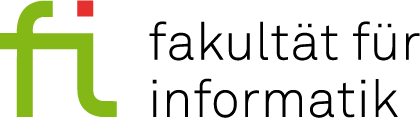
\includegraphics[height=0.08\textheight]{logos/fi_logo_german.png}\vspace{0.5cm}\newline
\vspace{-5cm}\newline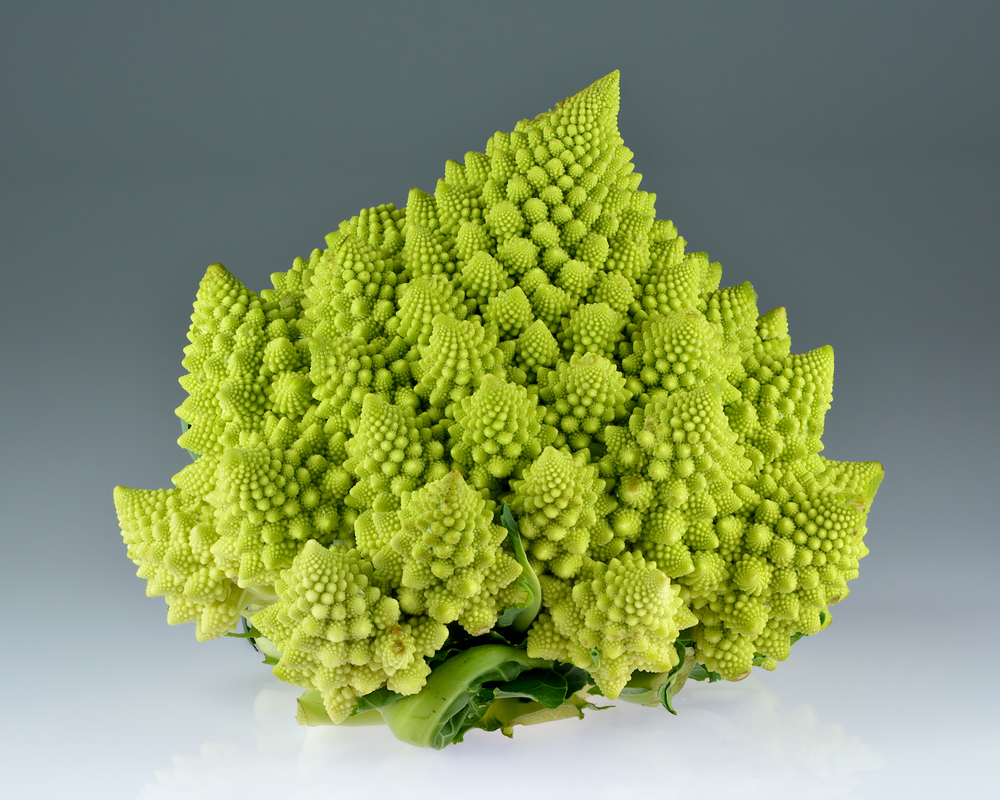
\includegraphics[height=0.33\textheight]{img/Romanesco_broccoli.jpg}\hspace{0.42\textwidth}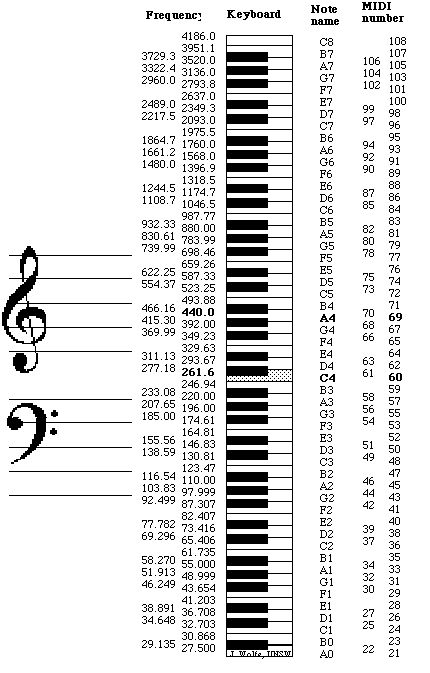
\includegraphics[height=0.65\textheight]{img/MIDI-numbers.jpg}\vspace{-6.5cm}\newline
	\thetitle}
\author{\theauthor}
% insert correct institute name
%\email{fabian.ostermann@tu-dortmund.de}
\date{\small\thedate\\\medskip\audioplayer{audio/speakertest.mp3}\vspace{-1cm}}
\institute{\theinstitute}
\subtitle{\vspace{0.25cm}\thesubtitle\vspace{-0.25cm}}
%\titlegraphic{}

\setbeamercolor{background canvas}{bg=white}
\setbeamercovered{invisible}
\usecolortheme[named=TUDoGreen]{structure}
\setbeamertemplate{frametitle}[default][center]
\setbeamerfont{frametitle}{size=\Large,series=\bfseries}
\setbeamerfont{framesubtitle}{size=\normalsize,series=\bfseries}

\usepackage{multicol}

%%%%%% draw at for drawing objects at specific positions
% https://tex.stackexchange.com/questions/82463/how-to-position-a-beamer-box-in-a-slide
\usepackage[absolute,overlay]{textpos}
\newcommand{\drawat}[2]{ % #1=x,y, #2=content
	\begin{textblock*}{0mm}(#1)
		#2
	\end{textblock*}
}
%%% the grid %%%
\usepackage[texcoord,
%grid,
gridunit=mm,gridcolor=black!10,subgridcolor=black!5,gridBG=false]{eso-pic}

%%%% make a file that lists all frametitles
\newwrite\slideinfofile
\immediate\openout\slideinfofile=slideinfo.txt
%\newcounter{SlideNumber}
\AtBeginEnvironment{frame}{
		\immediate\write\slideinfofile{%\theSlideNumber
		[\insertframenumber] \insertframetitle}
}

%%%%% Kommando für automatisch einblendendes Inhaltsverzeichnis am Anfang jeder Section
\newcommand{\toc}[1][currentsection]{
	\begin{frame}{Content}
		\only<1>{\tableofcontents[]}
		\only<2->{\tableofcontents[#1]}
	\end{frame}
}
\AtBeginSection[]{\toc}

%%% Useful Symbols %%%%
\usepackage{fontawesome}
\newcommand{\warnSign}{{\color{TUDoGreen}\faWarning}}
\newcommand{\conclude}{{\color{TUDoGreen}$\boldsymbol{\rightarrow}$}}
\newcommand{\Conclude}{{\color{TUDoGreen}$\boldsymbol{\Rightarrow}$}}
\newcommand{\questSign}{{\color{TUDoGreen}\fbox{\textbf{?}}}}
\newcommand{\attentionSign}{{\color{TUDoGreen}\fbox{\textbf{!}}}}
\newcommand{\ideaSign}{{\color{TUDoGreen}\fbox{\textbf{\faLightbulbO}}}}

\usepackage{musicography}
\renewcommand{\musEighth}{\musFlaggedNote{\symbol{7}}{\symbol{40}}}
%\musHalf already working


%% empty

\begin{document}

\setbeamertemplate{navigation symbols}{\scriptsize\insertframenumber\,/\,\inserttotalframenumber}
\maketitle
\setbeamertemplate{navigation symbols}{\scriptsize{\therunning}, \insertframenumber\,/\,\inserttotalframenumber}
\note{
	Hello everyone!
}

%\begin{frame}{One, Two, Mictest}
%	\centering
%	\audioplayer{speakertest.mp3}~~\color{TUDoGreen}\Large Können mich alle hören? \musEighth \musHalf
%\end{frame}

%%%%%%%%%%%%%%%%%%%%%%%%%%
% !TeX root = MDA_VL_Ostermann.tex
% !TeX spellcheck = en_US

\newcommand{\HIDE}[1]{}

\begin{frame}
	\centering
	{\color{TUDoGreen} \huge\textbf{Hello!}}\\
	\medskip
	\Large I am \textbf{Fabian Ostermann}
	
	\bigskip
	\begin{itemize}\setlength\itemsep{4pt}
		\normalsize
		\item PhD student at TU Dortmund, Germany, Chair for \emph{Computational Intelligence}\\
		\item B.Sc. and M.Sc. in Computer Science at TU Dortmund\\
		\item Studied jazz guitar at Folkwang University of the Arts, Essen, Germany
		\item[]
		\item[] Research on
		\begin{itemize}\setlength\itemsep{2pt}
			\item Computer Music \& Algorithmic Composition
			\item Human-centered Generative AI (Reinforcement Learning \& Evolutionary Algorithms)
			\item Procedural Content Generation \& Game-playing AI
		\end{itemize}
	\end{itemize}
\end{frame}

%%%%%%%%%%%%%%%%%%%%%%%%%%%%%%%%%%%
%%%%%%%%%%%%%%%%%%%%%%%%%%%%%%%%%%%
\section{Introduction and Motivation}

\begin{frame}[t]{Composition}
{\enquote{What is it?}}
	%vgl. 24.2.1 What Composers Do
	%-> Rückgriff auf Ebelings Folien: Was ist Musik?
	
	\underline{Hiller and Issacson} (1959) put it pragmatically:
	\begin{quote}
		\enquote{the act of composing can be thought of as the \textbf{extraction of order} out of a chaotic multitude of \textbf{available possibilities}} \citep[p.1]{HillerIssacson1959}
	\end{quote}
	
	\conclude~Hence: a \textbf{search problem}
	\bigskip
	
	\questSign~What is a (meaningful) \emph{search space}?
	
	\vspace{-.6cm}
	\hspace{-.3cm}
	\mbox{
		\raisebox{.5cm}{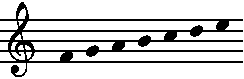
\includegraphics[height=1.2cm]{lily/Intro_pitches.pdf}}
		\raisebox{.5cm}{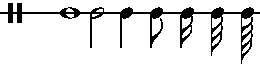
\includegraphics[height=.9cm]{lily/Intro_rhythms.pdf}}
		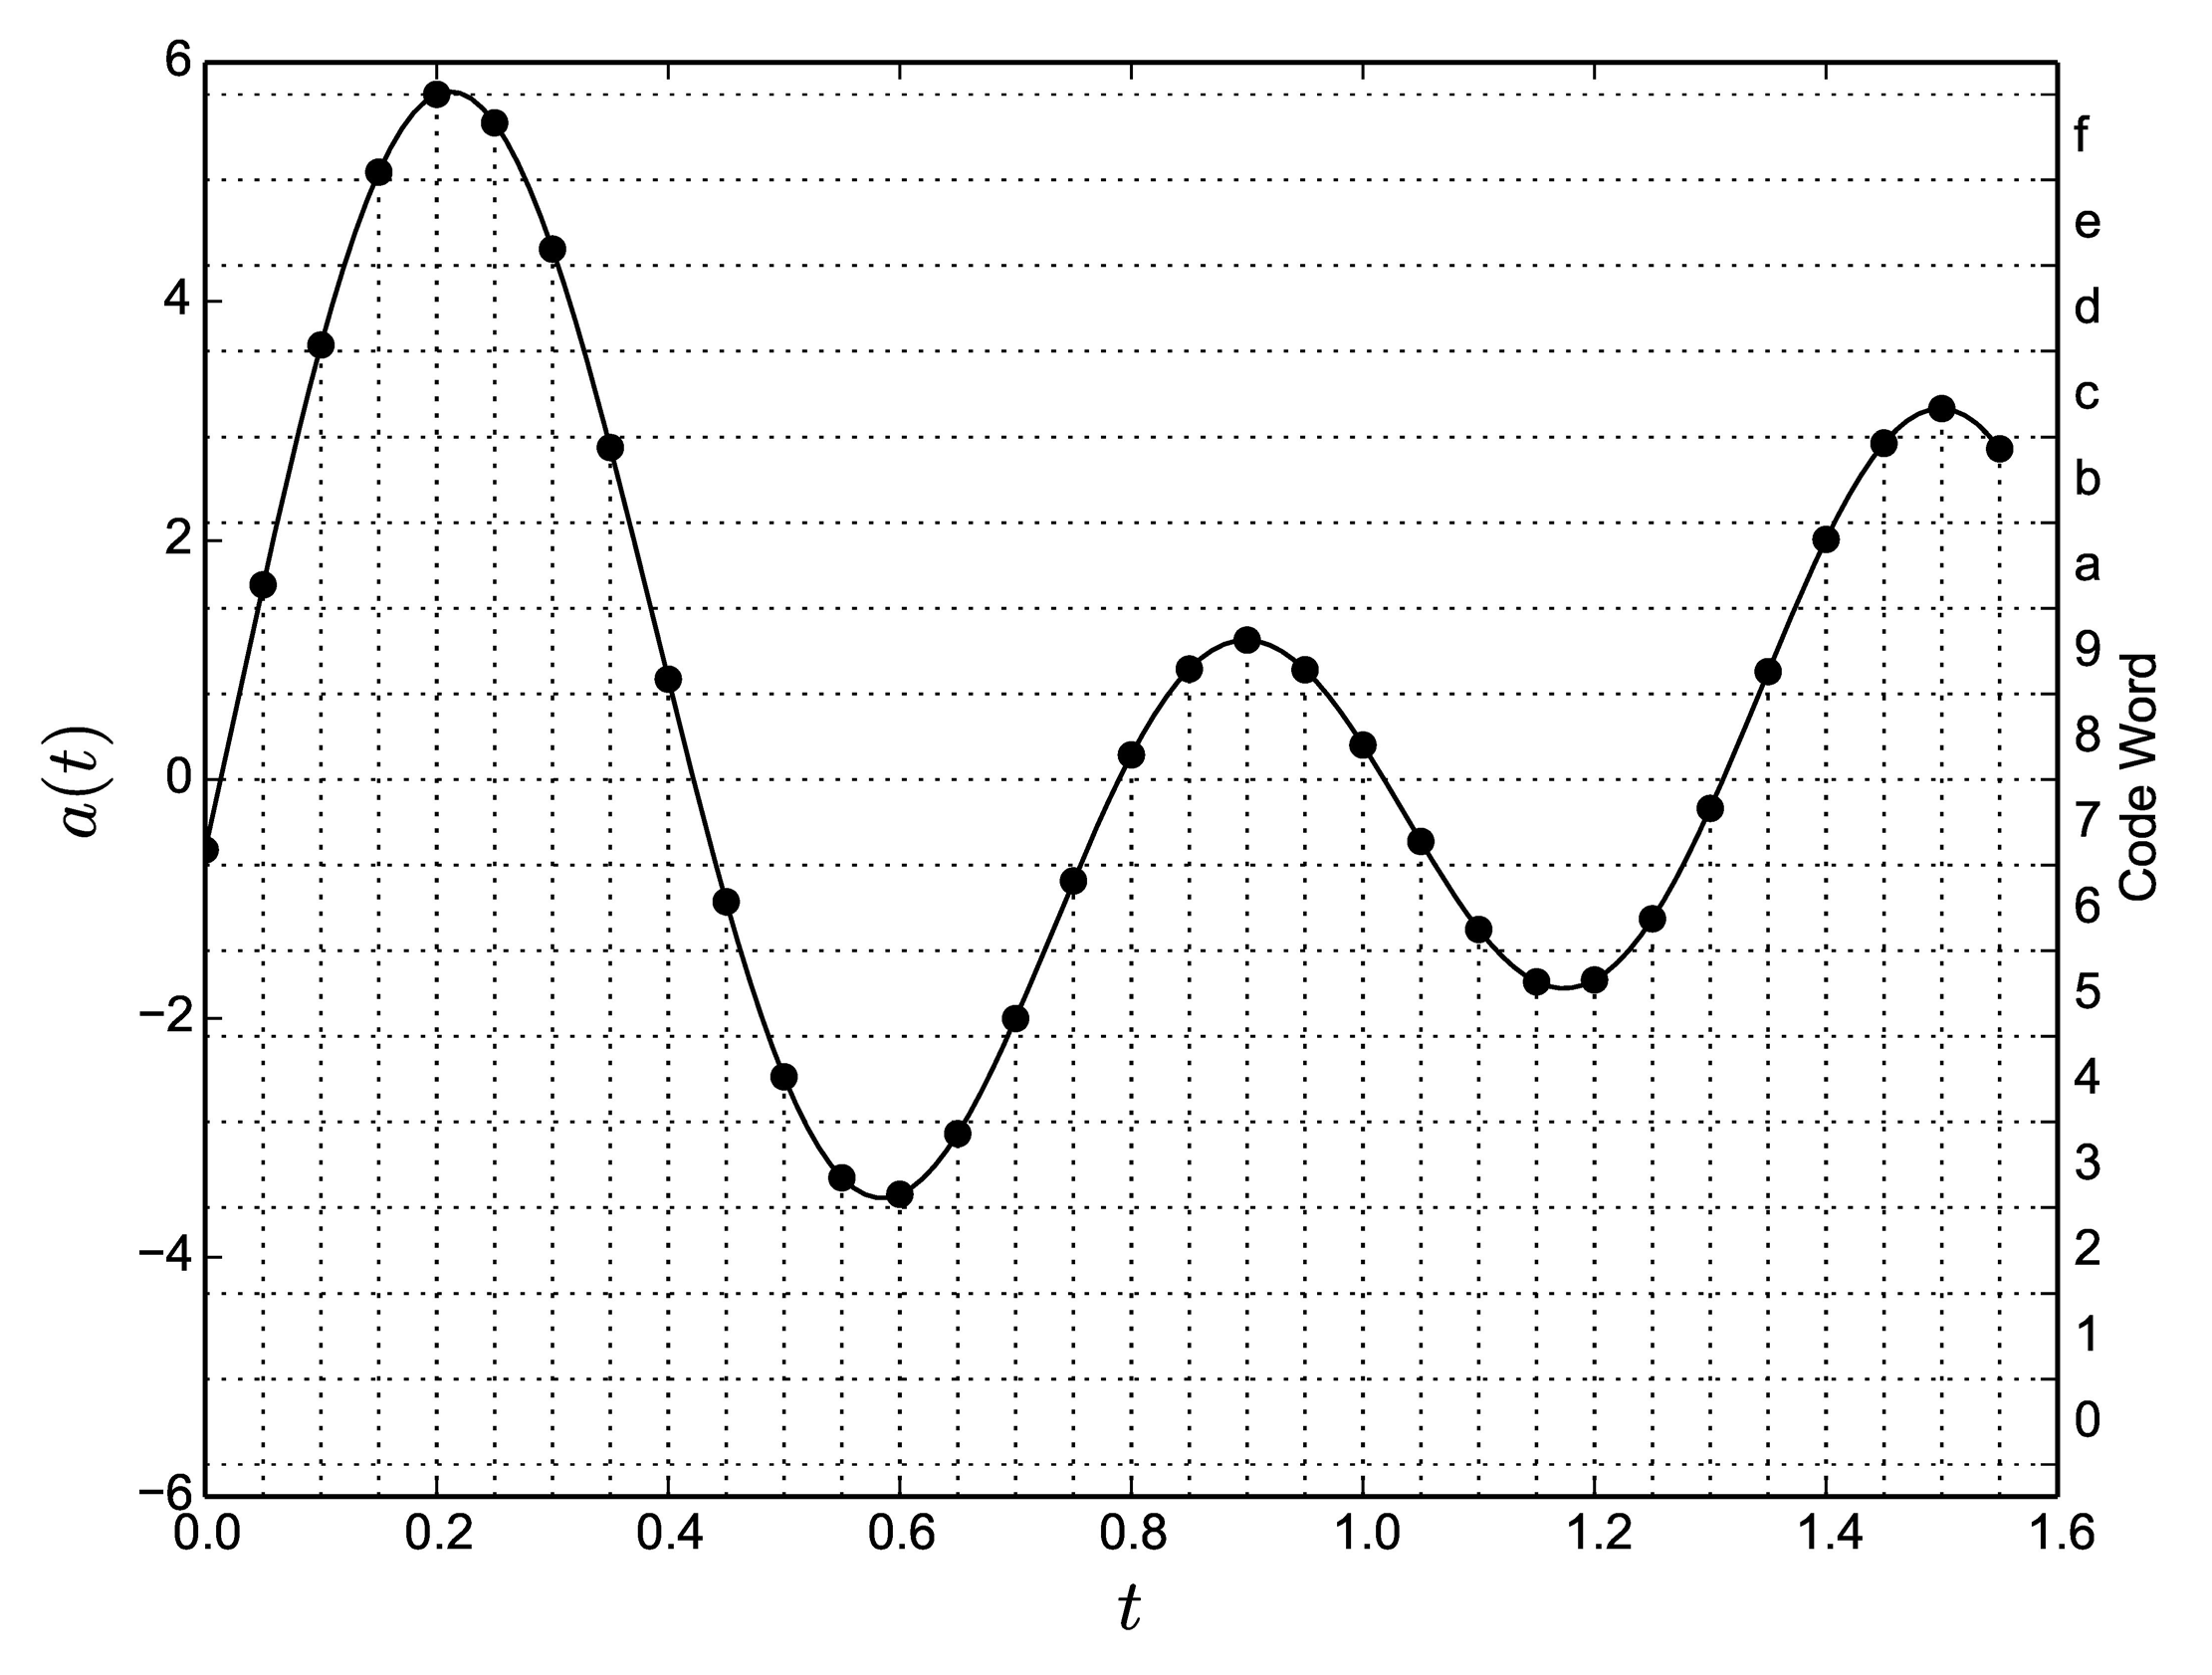
\includegraphics[height=2.6cm]{img/PCM_Waveform.png}
		\raisebox{.2cm}{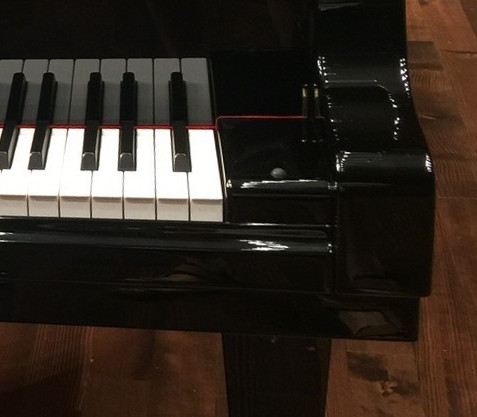
\includegraphics[height=2.1cm]{img/piano_edge.jpg}}
	}

	\medskip
	~~~~~~\conclude~Parameters of a \emph{tone}:~pitch, duration, loudness (intensity), timbre (quality), ...\\\medskip
	\hfill\Conclude~Very large in any case! (\emph{Combinatorial explosion})
\end{frame}

\HIDE{
\begin{frame}[t]{Automatic Composition}
{\enquote{What exactly is it?}}
	
	\begin{multicols}{2}
		\newcommand{\pointerleft}{{\color{TUDoGreen}\Large$\blacktriangleleft$}}
	\begin{infobox}[.45\textwidth]{Terminology}
		
		\textbf{Automat}ic Composition~~\visible<2>{\pointerleft}\\\medskip
		~~~vs.\\\medskip
		\textbf{Algorithm}ic Composition~~\visible<3>{\pointerleft}\\\medskip
		~~~vs.\\\medskip
		Computer Music~~\visible<4>{\pointerleft}
	\end{infobox}
	
	\columnbreak
	\only<2>{
		\begin{itemize}
			\item Autonomous machine
			\item Fully automatic
			\item[\Conclude] No input or control required
		\end{itemize}
	}
	\only<3>{
		\begin{itemize}
			\item[Def.] \emph{Algorithm} = \enquote{an unambiguous set of instructions for solving a problem}
			\item[\Conclude] \enquote{Generation of musical material by means of \textbf{unambiguous} instructions}\\ \hfill{\citep[p.513]{FernandezVico2013}}
			\item Thus: can be carried out manually by humans\\
			\conclude~\warnSign~not modern AI
		\end{itemize}
	}
	\only<4>{
		\begin{itemize}
			\item[\Conclude] \enquote{Any music in whose creation a computer was involved}
			\item So today, \textbf{almost everything}!
			\item[Ex.1:] Electronic music per se
			\item[Ex.2:] Traditional music productions are mixed on digital consoles
			\item[Ex.3:] Classical composers write scores in music notation software
			\item[\Conclude] The term is rather \textbf{useless}
		\end{itemize}
	}
	\end{multicols}

\end{frame}
}

\begin{frame}[t]{Motivation}
{\enquote{Why would anyone do this?}}
%vgl. 24.2.2 Why Automatic Composition?

	
	\underline{Plausible reasons}:
	\begin{itemize}
		\item Curiosity: \emph{homo ludens} (\enquote{the playing human} $\to$ \enquote{playing music}) % Ebeling Vorlesung
		\item New artistic paths and possibilities (\emph{experimentation})\\
		~~~\conclude~Creating vs. discovering \citep[p.591]{MDABook}
		\item Increases productivity (financial aspects, but also: \emph{creative flow})
	\end{itemize}
	\smallskip
	
	\underline{Controversy}:
	\begin{itemize}
		\item The topic sometimes meets with rejection\\
		~~~\conclude~can also be inspiring: \enquote{Boosting creativity by limitation}
		\item \enquote{Testing what is possible in order to understand what (perhaps) is not...?} \\
		~~~\conclude~What are the uniquely human qualities?
		\medskip
		\item[\Conclude] \underline{Today}: a mathematical/technical examination of different methods
	\end{itemize}
	%TODO \vspace{-3cm}\hfill\missingfig{Bild von einem Roboter der Musik spielt}
	
\end{frame}

\section{History}

\begin{frame}[t]{History without Computers}{Guido d'Arezzo (992--1050)}

	\drawat{12.6cm,.5cm}{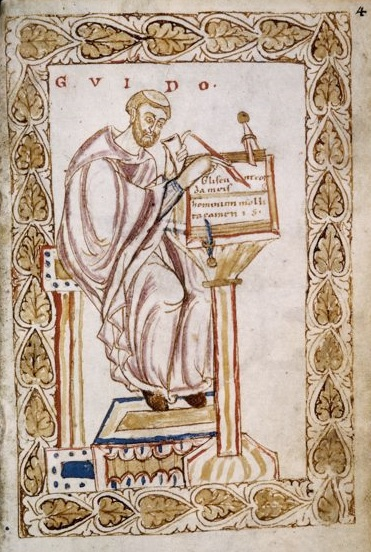
\includegraphics[height=.5\textheight]{img/Guido_van_Arezzo.jpg}}
	
	\begin{itemize}
		\item Monk, music theorist and teacher 
		\item Inventor of solmization (a technique for teaching singing)\\
		~~~\conclude~\enquote{do re mi fa so la si do}\\
		%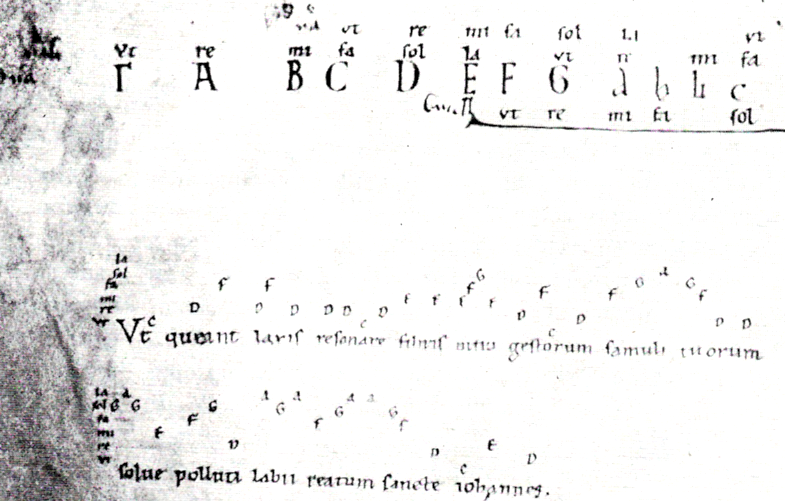
\includegraphics[height=.3\textheight]{img/Guido_van_Arezzo__Ut_queant_laxis.png}
	\end{itemize}
	
	\begin{infobox}[.75\textwidth]{Exercise for Arezzo's Students}
		Using a mapping that assigns to each vowel in $\{a,e,i,o,u\}$\\a note of a scale (e.g., C D E F G),\\any given text can be \enquote{transformed into music}.
	\end{infobox}

	\medskip
	\conclude~the first music algorithm in history (a so-called \textbf{Translational Model})

	\medskip
	\hfill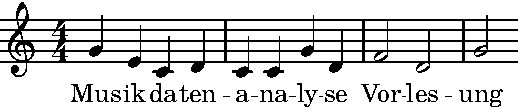
\includegraphics[height=1.5cm]{lily/Arezzo.pdf}\audioplayer{lily/Arezzo.midi}
\end{frame}

\begin{frame}{History without Computers}{Musical Dice Game}

	\begin{itemize}
	\item Inventor: Johann\,P. Kirnberger, 1757\\
	\hfill\conclude~popular pastime until the end of the 18th\,century
	\item Famous example: Wolfgang A. \textbf{Mozart}'s (1793) \citep[294d/516f]{KoechelVZ}\\
	~~~\enquote{Anleitung zum \textbf{Componieren von Walzern} vermittels zweier \textbf{Würfel}} 
	\end{itemize}	
	
	\begin{multicols}{2}
	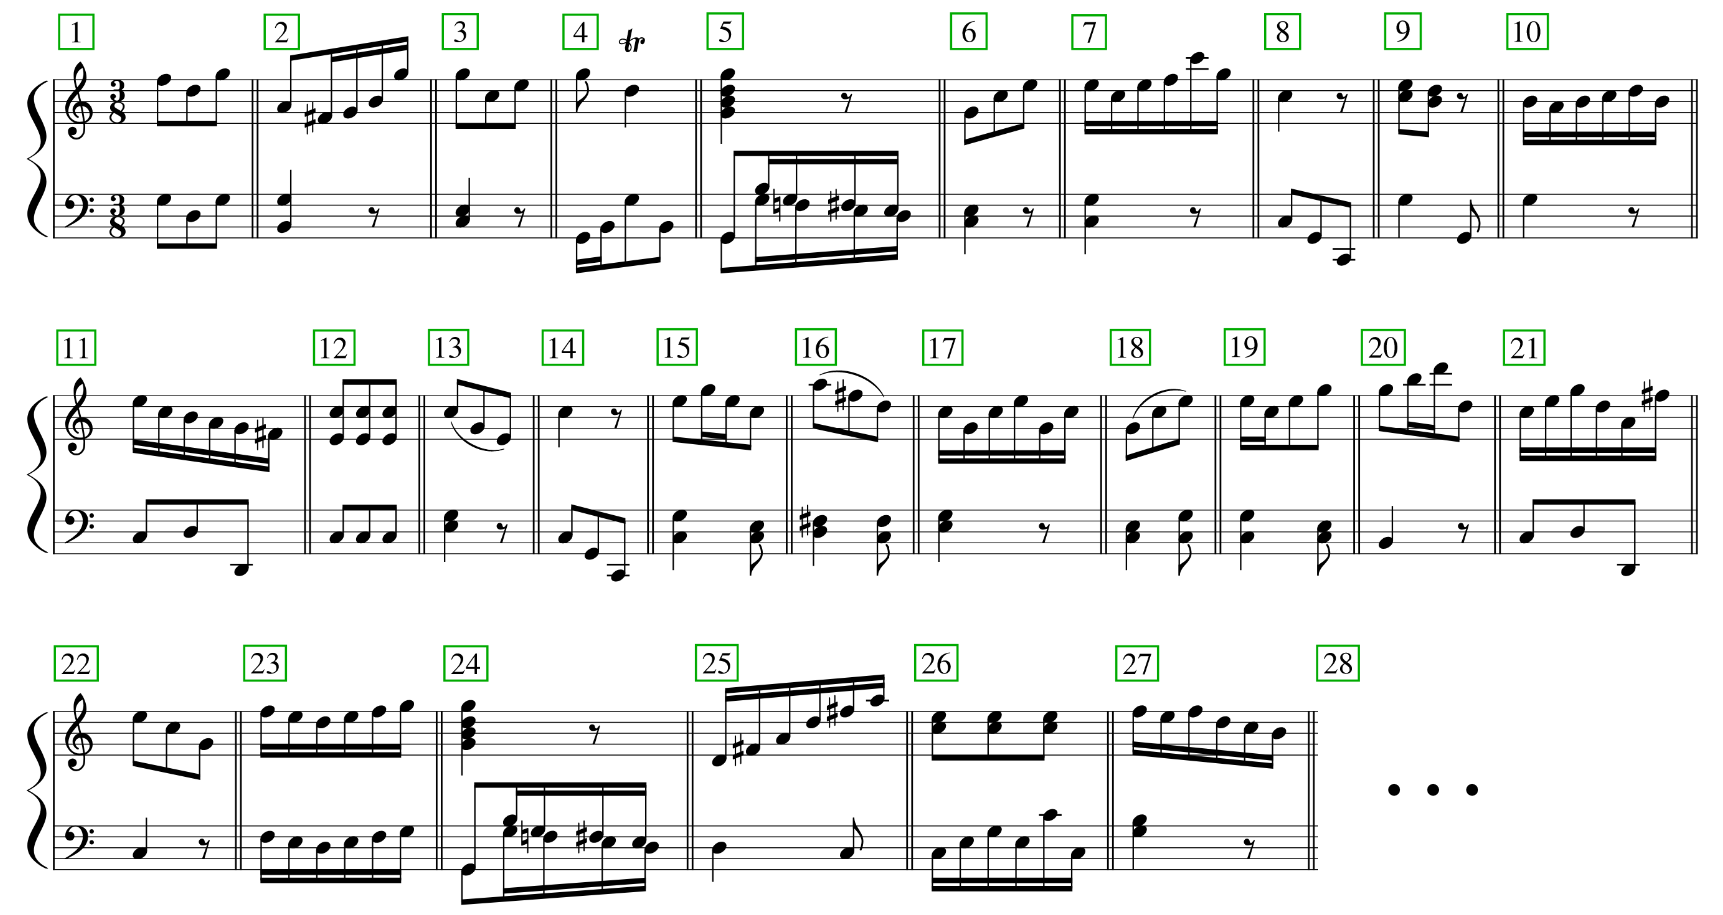
\includegraphics[width=.52\textwidth]{img/Wuerfelspiel_Noten.png}
	
	~~\resizebox{.45\textwidth}{!}{
		\csvreader[tabular=|r|rrrrrr|,
		table head=\toprule,
		table foot=\bottomrule,
		no head,
		late after line=\\,
		late after first line=\\\midrule,]{img/Wuerfelspiel_Zahlentafel.csv}{}{
			\csvcoli & \csvcolii & \csvcoliii & \csvcoliv & \csvcolv
			%& \csvcolvi & \csvcolvii & \csvcolviii
			& \large{$\boldsymbol{\cdots}$} & \csvcolxvii
		}
	}
	\end{multicols}

	\hfill \footnotesize Interactive version: \href{https://www.buschs.de/Mozart/}{\texttt{https://www.buschs.de/Mozart/}}
	
\end{frame}

\begin{frame}{History without Computers}{Serial Music}
	\begin{itemize}
		\item From around 1948: generalization of the \emph{twelve-tone technique} (1920)\\
		\hfill {\footnotesize by Arnold Schoenberg (1874--1951)}
		\item Purpose: liberation from redundancy, arbitrariness and \emph{personal taste} (!)
		\item Not only pitch, but also duration, loudness, articulation and timbre are determined by predefined \emph{series}
		
		\bigskip
		\underline{Simple example:}\\
		\medskip
		
		\mbox{
			\hspace{-1cm}
			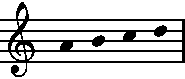
\includegraphics[height=1cm]{lily/SerielleMusik_pitches.pdf}
			~\raisebox{.3cm}{$\Large\boldsymbol{*}$}
			~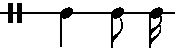
\includegraphics[height=.6cm]{lily/SerielleMusik_rhythms.pdf}
			~\raisebox{.3cm}{$\Large\boldsymbol{=}$}
			~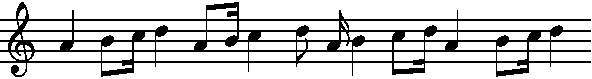
\includegraphics[height=1cm]{lily/SerielleMusik_folded_nobars.pdf}
		}
	
		\bigskip
		\hfill \raisebox{.3cm}{Embedding in 4/4 time:}
		~~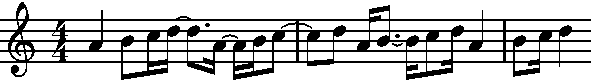
\includegraphics[height=1cm]{lily/SerielleMusik_folded.pdf}
		\audioplayer{lily/SerielleMusik_folded.midi}
	\end{itemize}

\end{frame}

\begin{frame}{History without Computers}{Serial Music II}
	
	\vspace{-.8cm}
	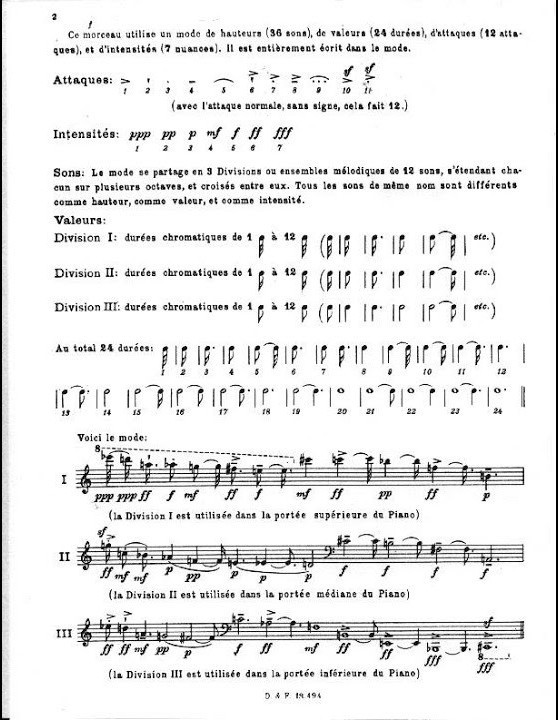
\includegraphics[width=.32\textwidth]{img/Olivier_Messiaen_Regeln.jpg}
	\hfill\raisebox{2.5cm}{\Huge\Conclude}~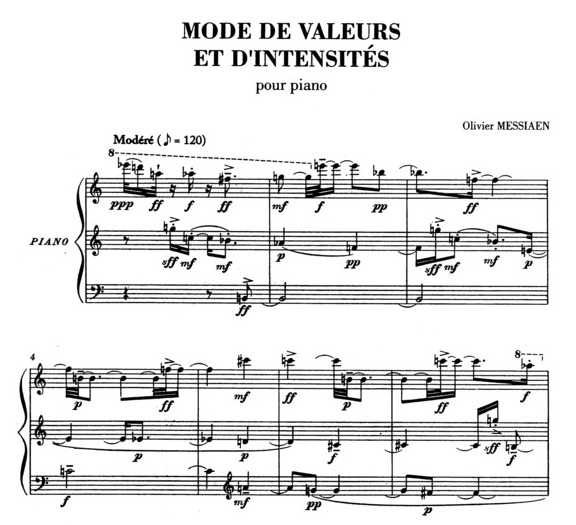
\includegraphics[width=.44\textwidth]{img/Olivier_Messiaen_Score.png}\audioplayer{audio/Olivier_Messiaen-Mode_de_valeurs_et_d_intensites.mp4}~~
	
	\begin{itemize}
		\item[\conclude] (Very) strict rules $\hat=$ sets of instructions (algorithms)
		\item[\Conclude] Reception: complex structures can no longer be grasped by ear\\
		\hfill {\small (a problem that automatic composition inherits!)}
	\end{itemize}
	
	%Empfehlung: Olivier Messiaen: \emph{Mode de valeurs et d'intensités} (1949) \url{youtube.com/watch?v=tG9TAqBZa4}
\end{frame}

%\begin{frame}{Geschichte ohne Computer}{Serielle Musik}
%TODO
%	\todobox{Zeige Babbitt Square, um zu zeigen -> haben es sehr weit getrieben\\
%	Mathe darunter?}
%\end{frame}

\begin{frame}{History with Computers}{Iannis Xenakis (1922--2001) -- \emph{Stochastic} Music}
	
	Xenakis explores existing mathematical models
	\medskip
	
	\enquote{Achorripsis} (1957) is based on the Poisson distribution $P_\lambda(k) = \frac{\lambda^k}{k!}e^{-\lambda}$
	% https://www.iannis-xenakis.org/en/stochastic-music/
	
	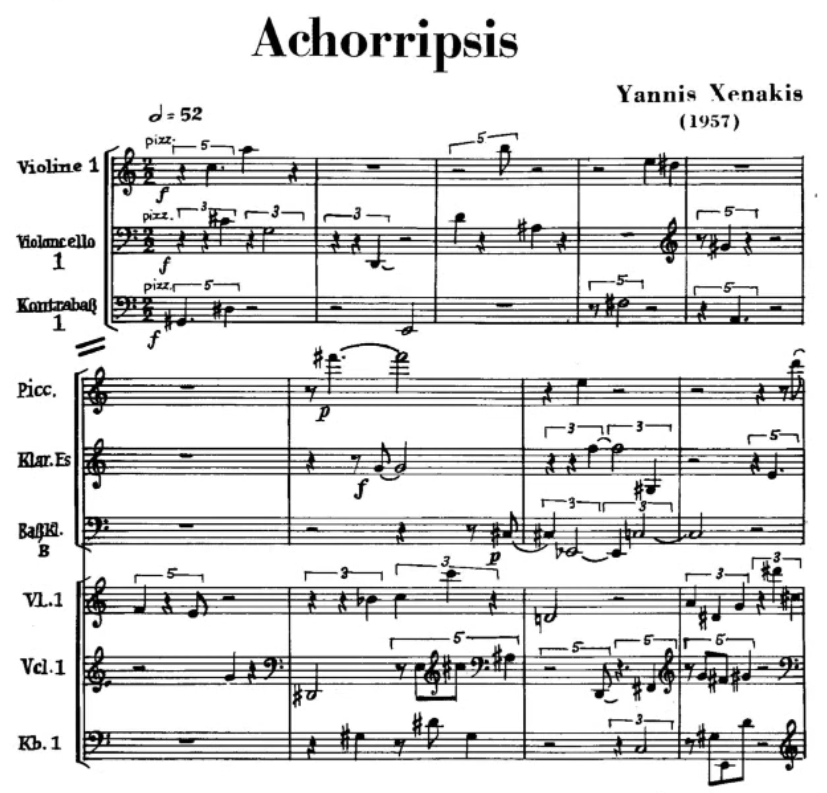
\includegraphics[width=.33\textwidth]{img/Achorripsis_Noten.png}
	~~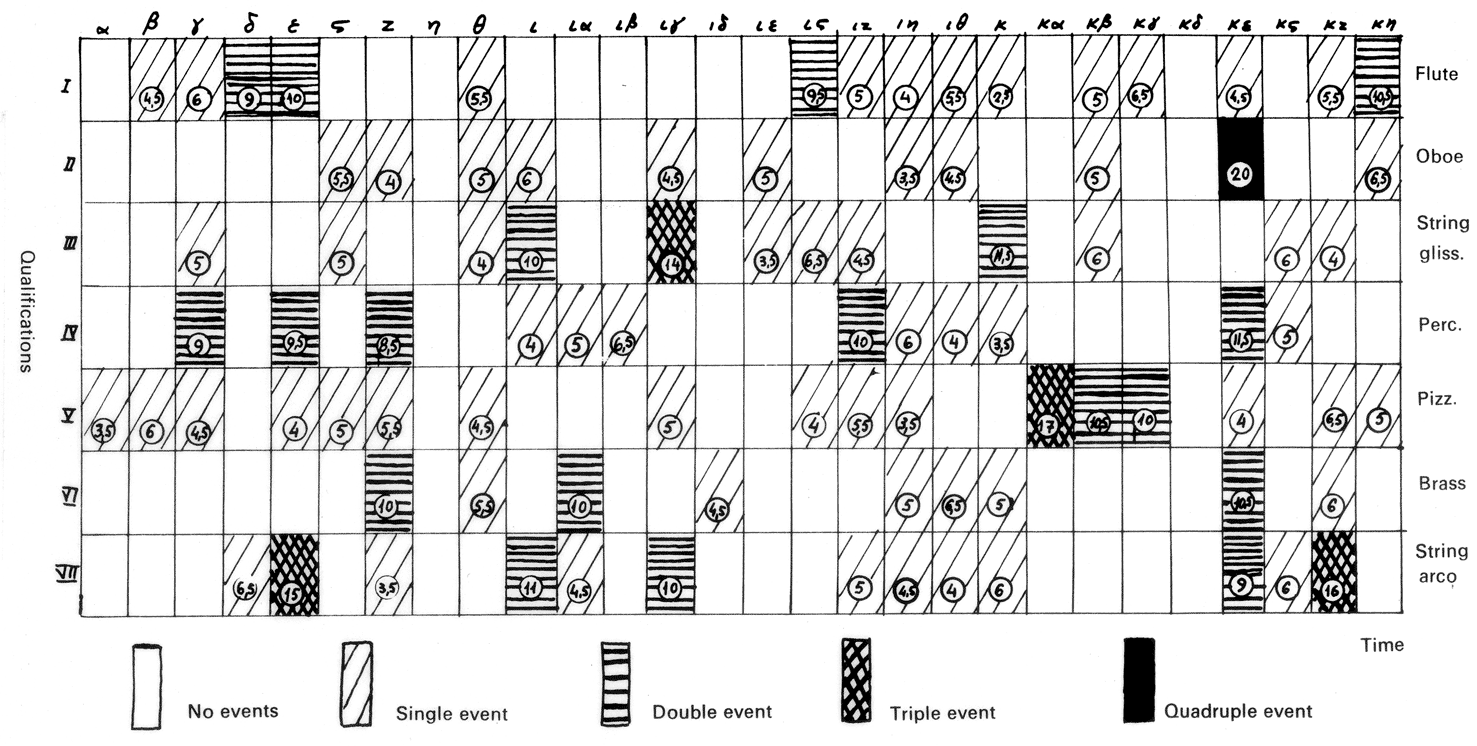
\includegraphics[width=.6\textwidth]{img/Achorripsis_CellMatrix_from_FormalizedMusic.png}\\
	
	\medskip
	\hfill\conclude~complexity later exceeded \textbf{manual \enquote{computability}}\\
	
	%Erklärung und Literaturverweise: second.wiki/wiki/achorripsis
	%Score: youtube.com/watch?v=rEyqJPW3Hi8
	%Visualisierung: youtube.com/watch?v=WasFTDq0dJI
\end{frame}

\begin{frame}[t]{History with Computers}{Illiac Suite, String Quartet No. 4 (1957)}
	
	\drawat{11.5cm,2.5cm}{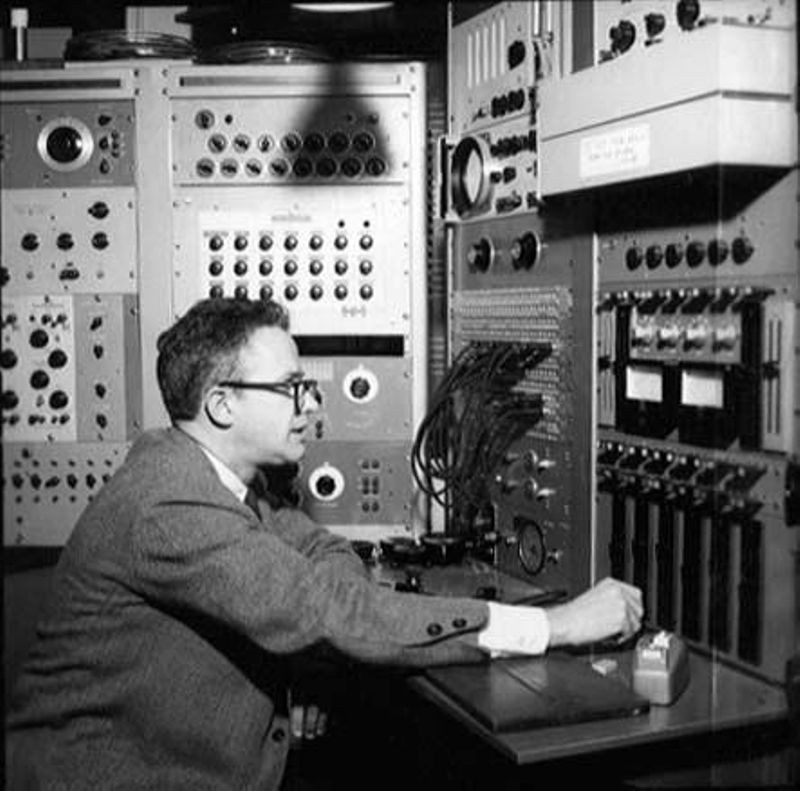
\includegraphics[width=4cm]{img/hiller.jpg}}
	\drawat{11.5cm,6cm}{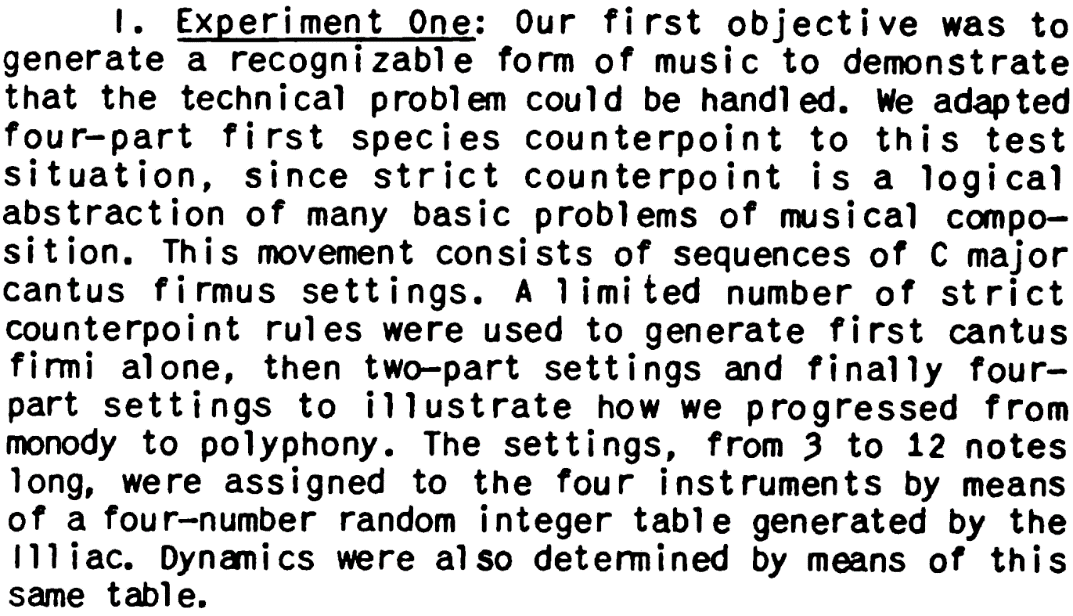
\includegraphics[width=4cm]{img/Hiller-exp1-text.png}}
	
	\begin{itemize}
		\item Considered the \enquote{first serious attempt} at computer-aided composition
		\item by Lejaren Hiller and Leonard Isaacson, University of Illinois
		\item Four movements:
		\begin{enumerate}
			\item \emph{cantus firmi}
			\item Four-part writing with compositional rules
			\item Experiment with rhythm, dynamics and articulation \audioplayer{audio/Lejaren_Hiller_-_Illiac_Suite_for_String_Quartet_3of4.mp3}
			\item Simple stochastic models
		\end{enumerate}
	\end{itemize}
	
	\bigskip
	\attentionSign~Performed by human musicians (string quartet)

	
\end{frame}

\begin{frame}{History with Computers}{Band-In-A-Box (1990)}
	\centering
	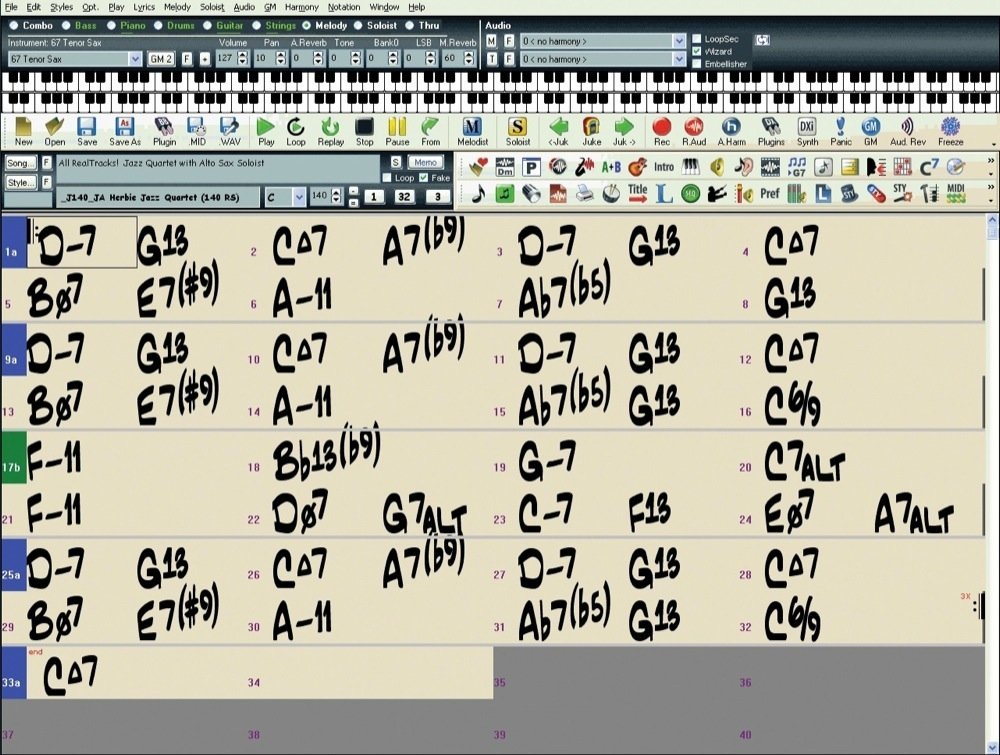
\includegraphics[width=.6\textwidth]{img/bandinabox.jpg}
	\parbox{0.3\textwidth}{
		\begin{itemize}
			\vspace{-2cm}
			\item public attention
			\item commercial breakthrough
		\end{itemize}
		\audioplayer{audio/BandInABox_1999.mp4}
	}
\end{frame}


%%%%%%%%%%%%%%%%%%%%%%%%%%%%%%%%%%%%%%%%%%%%%%%%%%%%%%
%%%%%%%%%%%%%%%%%%%%%%%%%%%%%%%%%%%%%%%%%%%%%%%%%%%%%%
\section{Categorizations \& Examples}
\newcommand{\dimOneTitle}{Automatic vs. algorithmic}
\newcommand{\dimTwoTitle}{Deterministic vs. stochastic}
\newcommand{\dimThreeTitle}{Rule-based vs. data-driven}
\newcommand{\dimFourTitle}{Output: scores vs. sounds}
\newcommand{\dimFiveTitle}{Goal/effort/ambition}
\newcommand{\dimSixTitle}{Static/autonomous/aleatoric vs. adaptive/interactive/real-time/human-in-the-loop}

\begin{frame}[t]{Proposed Categorizations}
	\vspace{-.5cm}
	\begin{center}
		No consensus in the literature (so far).
	\end{center}
	%\medskip
	
	Proposals:
	\begin{itemize}
		\item[\textbf{I.}] \dimOneTitle 
		\item[\textbf{II.}] \dimTwoTitle
		\item[\textbf{III.}] \dimThreeTitle
		\item[\textbf{IV.}] \dimFourTitle
		\item[\textbf{V.}] \dimFiveTitle
		\item[\textbf{VI.}] \dimSixTitle
	\end{itemize}
	\medskip
	
	\begin{itemize}
		\item[\warnSign] These \enquote{dimensions} are not (necessarily) orthogonal.
		\item[\warnSign] This list makes no claim to completeness.
	\end{itemize}
\end{frame}

\begin{frame}{II. \dimTwoTitle}{Lindenmayer System (deterministic)}
	An L-system is a quadruple $G=(V,S,\omega,P)$, where
	\begin{itemize}
		\item $V$ is a set of (replaceable) \textbf{variables},
		\item $S$ is a set of (non-replaceable) symbols,
		\item $\omega$ is a start word (axiom), and
		\item $P$ is a set of \textbf{production rules}.
	\end{itemize}

	\begin{multicols}{2}
		\underline{An example}:\\
		\begin{itemize}
			\item[] Let $V = \{a,b\},~S=\emptyset,~\omega=a$.
			\item[] Let $P$ consist of
			\item[] ~~~$a \mapsto b$
			\item[] ~~~$b \mapsto ab$
		\end{itemize}
	\columnbreak

		\begin{itemize}
			\footnotesize
			\item[n=0:] a
			\item[n=1:] b
			\item[n=2:] ab
			\item[n=3:] bab
			\item[n=4:] abbab
			\item[n=5:] bababbab
			\item[\dots] etc.
		\end{itemize}
	\end{multicols}

	\drawat{11.5cm,4.7cm}{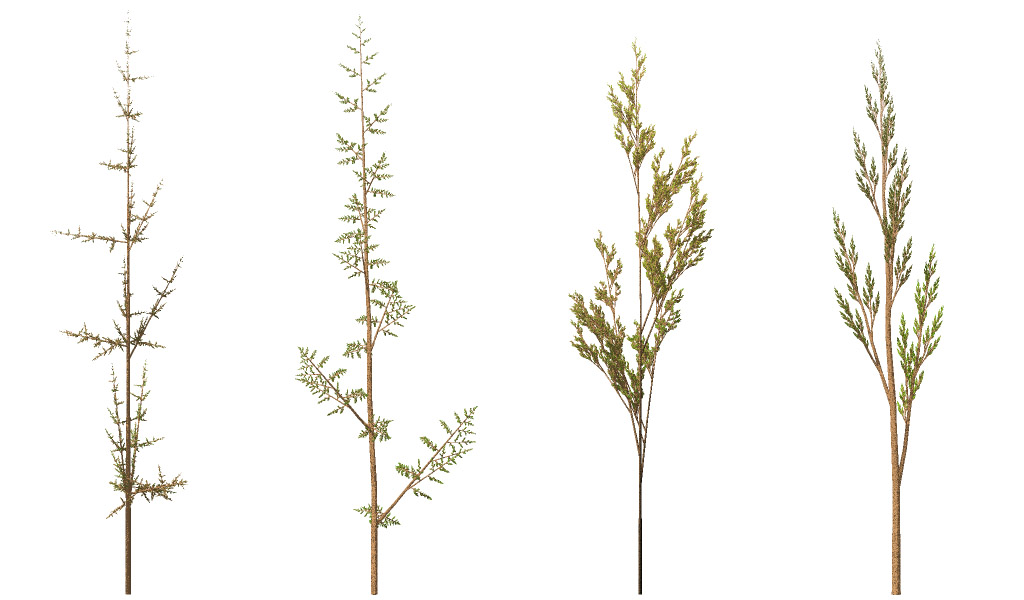
\includegraphics[height=.4\textheight]{img/Fractal_weeds.jpg}}
\end{frame}

\begin{frame}{II. \dimTwoTitle}{Lindenmayer System II}
	\parbox{.25\textwidth}{
		\begin{itemize}
			\scriptsize
			\item[n=0:] a
			\item[n=1:] b
			\item[n=2:] ab
			\item[n=3:] bab
			\item[n=4:] abbab
			\item[n=5:] \fbox{bababbab}
			\item[\dots] etc.
		\end{itemize}
	}
	\parbox{.6\textwidth}{
		\raisebox{.5cm}{(1)~\audioplayer{lily/LSystem_1.midi}}~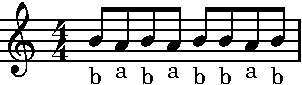
\includegraphics[height=1.3cm]{lily/LSystem_1.pdf}
		
		\medskip
		\raisebox{.7cm}{(2)~\audioplayer{lily/LSystem_2.midi}}~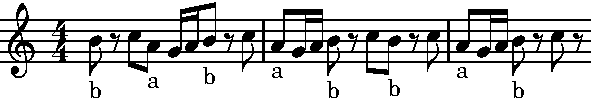
\includegraphics[height=1.5cm]{lily/LSystem_2.pdf}
		
		\medskip
		\raisebox{.7cm}{(3)~\audioplayer{lily/LSystem_3.midi}}~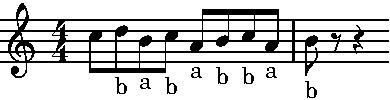
\includegraphics[height=1.5cm]{lily/LSystem_3.pdf}
	}
	
	\bigskip
	\bigskip
	\hfill\Conclude~The final result depends heavily on the \emph{letter-to-music mapping}

	\HIDE{
		\bigskip
		\hrule
		\bigskip
		Determinism never accurately simulates the human compositional process\\
		\hfill\conclude~random processes such as intuition and \enquote{happy accidents} are missing
	}
\end{frame}

\begin{frame}{II. \dimTwoTitle}{Fractals (deterministic)}
	\drawat{2cm,3cm}{\parbox{3cm}{Romanesco\\(cauliflower)}}
	\begin{center}
		~~~~~~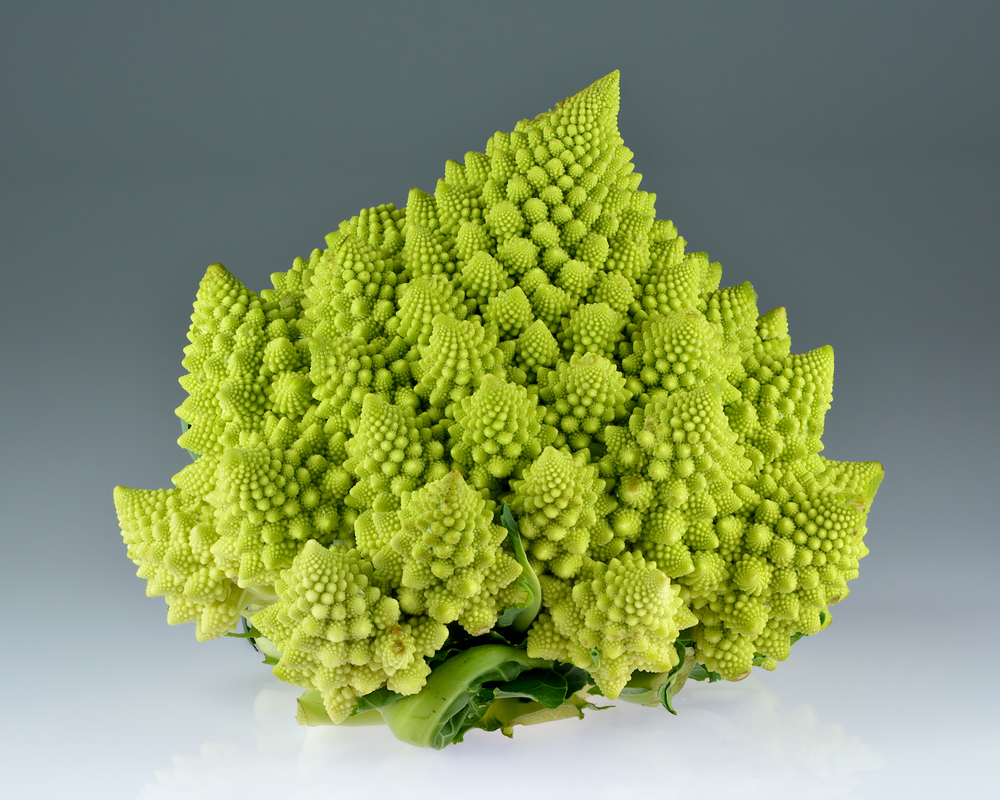
\includegraphics[width=.55\textwidth]{img/Romanesco_broccoli.jpg}
	\end{center}
\end{frame}

\begin{frame}{II. \dimTwoTitle}{Gary Lee Nelson -- \enquote{Fractal Mountains} (1988--89)}
	Example of generating pitches with fractals:
	
	\begin{center}
	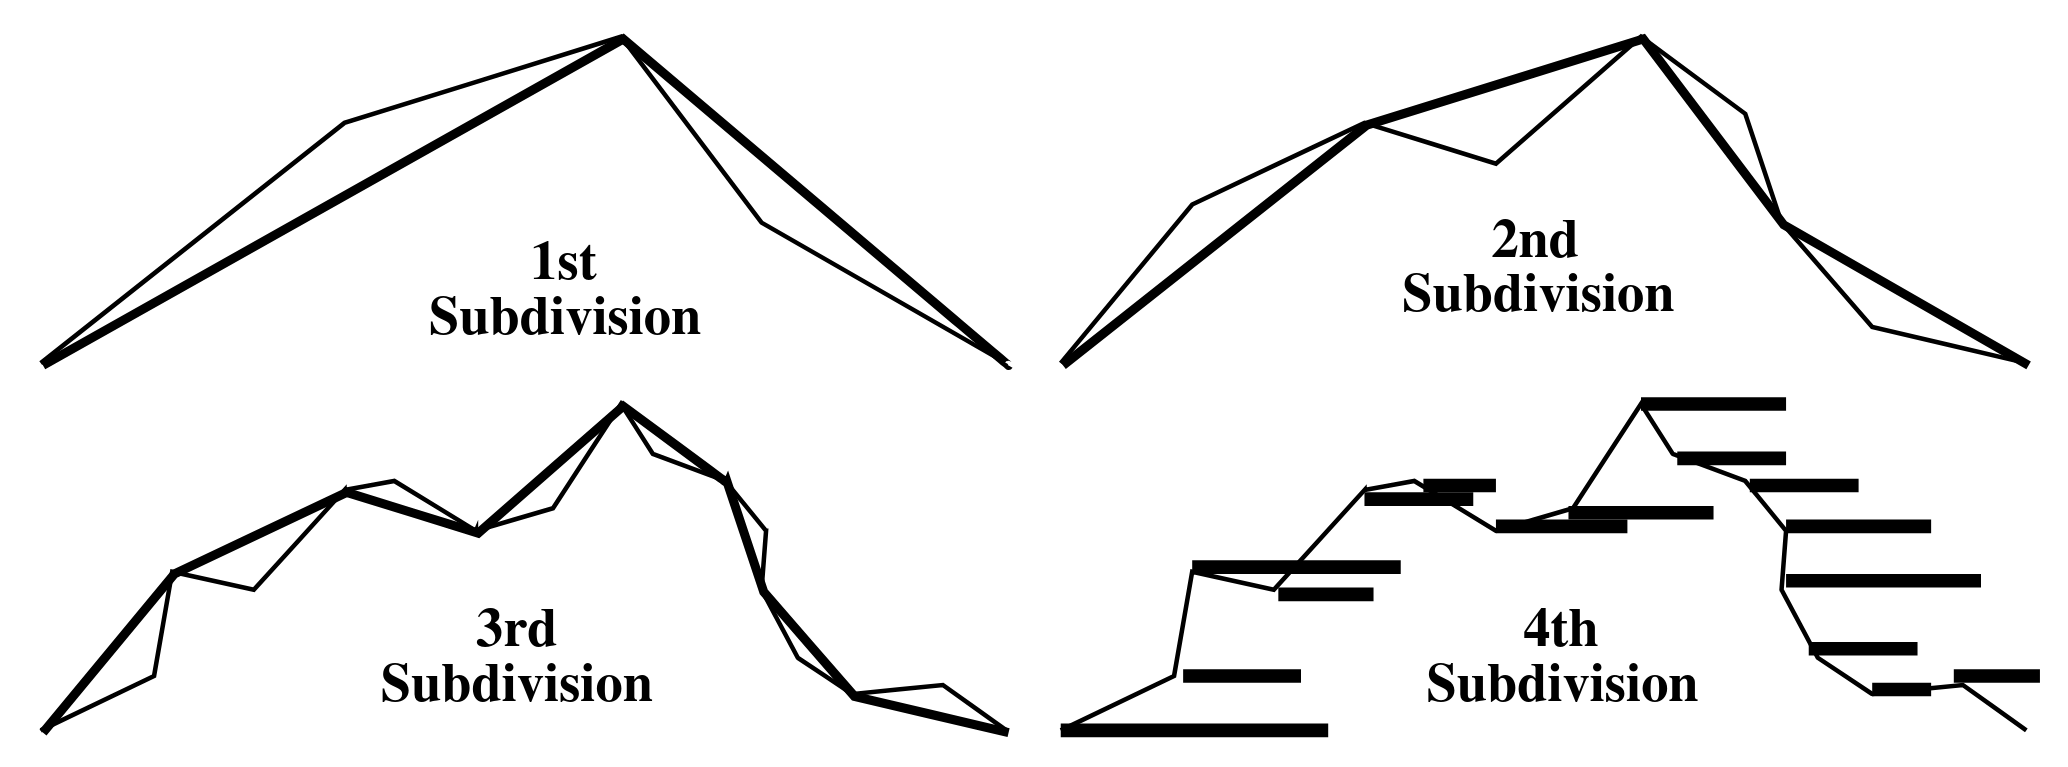
\includegraphics[width=.8\textwidth]{img/Fractal_Mointain.png}
	\end{center}
	
	\conclude~96 pitch steps per octave\\
	Further fractal functions for note duration and loudness
	
	\hfill\tiny\url{youtube.com/watch?v=KV3V3c8mqGs}\\
	\hfill\url{timara.oberlin.edu/gnelson/PapersPDF/GNfract.pdf}
	
\end{frame}

\begin{frame}{II. \dimTwoTitle}{Markov Chain (stochastic)}
	A Markov chain is a \emph{stochastic process}
	\begin{center}
		{$=$ math. description of temporally ordered random events} (e.g., stock prices)
	\end{center}

	\underline{Markov property}:
	\begin{center}
		$P(X_{t+1} = s_{j_{t+1}} | X_t = s_{j_t}, X_{t-1} = s_{j_{t-1}},\dots,X_{0} = s_{j_0}) = P(X_{t+1} = s_{j_{t+1}} | X_t = s_{j_t})$
	\end{center}

	\conclude~The next state depends \underline{only} on the current state (\enquote{memorylessness})

\end{frame}

\begin{frame}{II. \dimTwoTitle}{Markov Chain (Example 1)}
	
	\parbox{.6\textwidth}{
		\centering
		\underline{Hänschen Klein}
		\fbox{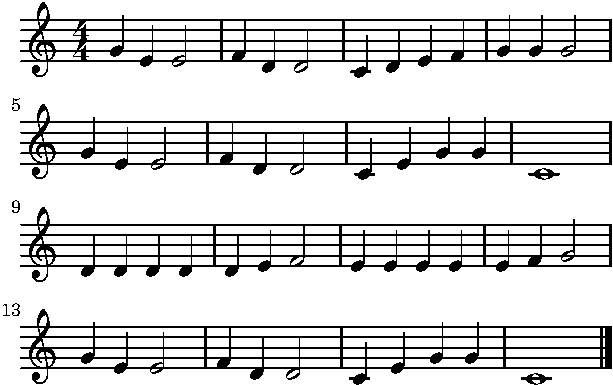
\includegraphics[width=.5\textwidth]{lily/HaenschenKlein.pdf}}
	}
	\parbox{.39\textwidth}{
		49 notes\\
		5x C, 12x D, 15x E, 6x F, 11x G\\
		
		\begin{itemize}
			\item $P(X=C) = \frac{5}{49} = 10.2\%$
			\item $P(X=D) = \frac{12}{49} = 24.5\%$
			\item $P(X=E) = \frac{15}{49} = 30.6\%$
			\item $P(X=F) = \frac{6}{49} = 12.2\%$
			\item $P(X=G) = \frac{11}{49} = 22.4\%$
		\end{itemize}
	}

	\hfill \Conclude~\raisebox{-.25cm}{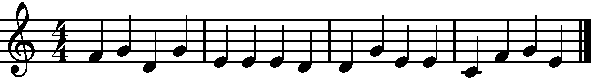
\includegraphics[height=.8cm]{lily/HaenschenKlein_random.pdf}}\,\audioplayer{lily/HaenschenKlein_random.midi}
	
	\medskip
	\hfill \warnSign~No conditioning at all (no chain)
	
	% 6x c, 12x d, 15x e, 6x f, 11x g
\end{frame}

\begin{frame}{II. \dimTwoTitle}{Markov Chain (Example 2)}
	
	\mbox{
		\parbox{.54\textwidth}{
			\centering
			\underline{Hänschen Klein}
			\fbox{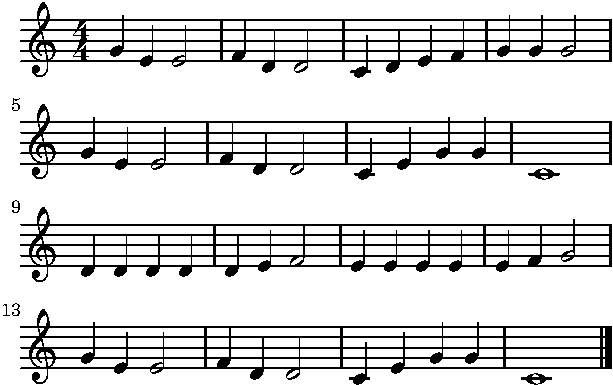
\includegraphics[width=.5\textwidth]{lily/HaenschenKlein.pdf}}
		}
		\parbox{.5\textwidth}{
			Markov property:
			
			\begin{itemize}
				\item $P(X_{t+1} = C | X_{t} = C) = 0$
				\item[] ~~$\vdots$
				\item $P(X_{t+1} = G | X_{t} = G) = \frac{6}{48} \small= 12.5\%$
				\item[] ~~$\vdots$
				\item $P(X_{t+1} = E | X_{t} = G) = \frac{3}{48} \small= 6.25\%$
			\end{itemize}
		}
	}

	\medskip
	\hspace{4.5cm}\underline{Extension}, e.g., to relative intervals, rhythm, ...\\
	\hspace{4.5cm}\underline{Increasing dependencies}: n-th order Markov chain\\
	\smallskip
	\hspace{4.5cm}\underline{Learning method}: \emph{Hidden Markov Model}
	
\end{frame}

\begin{frame}{II. \dimTwoTitle}{Markov Chain (Listening Examples)}
	
	Beethoven \enquote{Für Elise} \audioplayer{audio/elise_detailed.mp3}\\
	\bigskip
	Markov chain,~~1st~order \audioplayer{audio/elise_detailed_markov_1.mp3}\\
	\smallskip
	Markov chain,~~3rd~order \audioplayer{audio/elise_detailed_markov_3.mp3}\\
	\smallskip
	Markov chain,~~5th~order \audioplayer{audio/elise_detailed_markov_5.mp3}\\
	\smallskip
	Markov chain,~10th~order \audioplayer{audio/elise_detailed_markov_10.mp3}\\
	
	\vfill\footnotesize
	\parbox{.44\textwidth}{
		Jupyter notebook for reproduction:\\
		\url{https://github.com/lpensel/multiply-surrender/tree/master/Markov_Music}
	}
	
	\drawat{8.2cm,1.8cm}{
		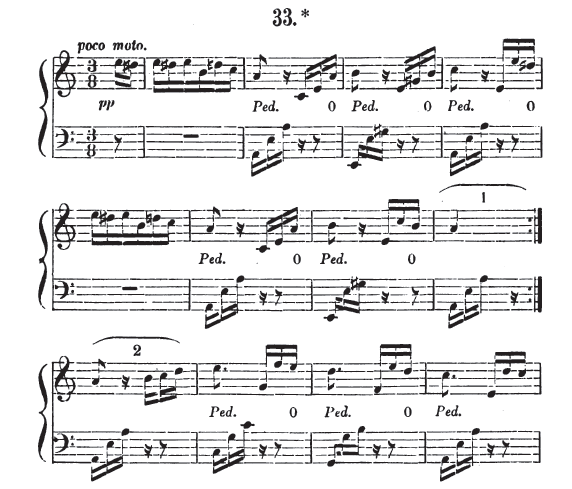
\includegraphics[width=7cm]{img/FuerElise_Erstausgabe_1867_crop.png}
	}
\end{frame}

\begin{frame}{III. \dimThreeTitle}{Kemal Ebcio\u{g}lu: CHORAL Project (rule-based)}
	\textbf{Expert systems} (also \enquote{knowledge-based} systems) implement identified/known rules as a (logic) program.
	\medskip
	
	\vspace{-.5cm}
	\mbox{\underline{Example task}: four-part harmonization in the style of J.\,S.\,Bach. \raisebox{-.5cm}{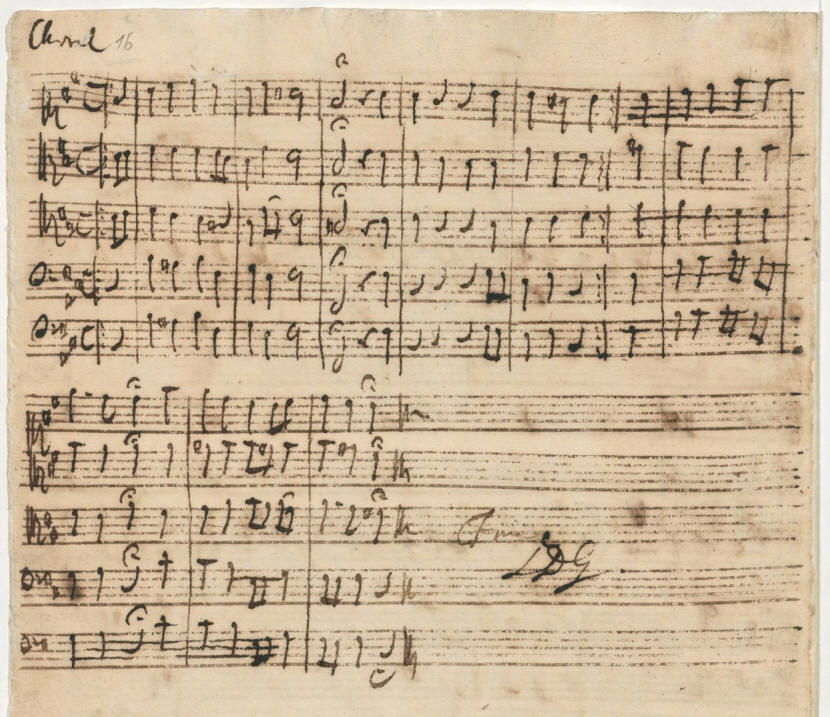
\includegraphics[height=1.5cm, clip, trim=0cm 20cm 0cm 3cm]{img/bwv84_choral_autograph.png}}}
	\medskip
	
	\begin{quote}
	\enquote{The rules and \textbf{heuristics} were found mainly from empirical observation of the
		chorales and personal intuitions, although we used a number of \textbf{traditional treatise}} {\footnotesize\citep[p.73]{CHORAL_report}}\\
	\end{quote}
	{\color{TUDoGreen}\textbf{Def.}} \emph{Heuristic}: a set of instructions whose correctness is grounded in empirical evidence or intuition and whose result is not necessarily optimal.
	\medskip
	
	Rules in classical composition treatises are typically heuristics, since they never hold without exception (e.g., the \emph{prohibition of parallel fifths}).
\end{frame}
\begin{frame}[t]{III. \dimThreeTitle}{CHORAL Project (1986): 350 Rules (\warnSign)}
	\parbox{.7\textwidth}{
		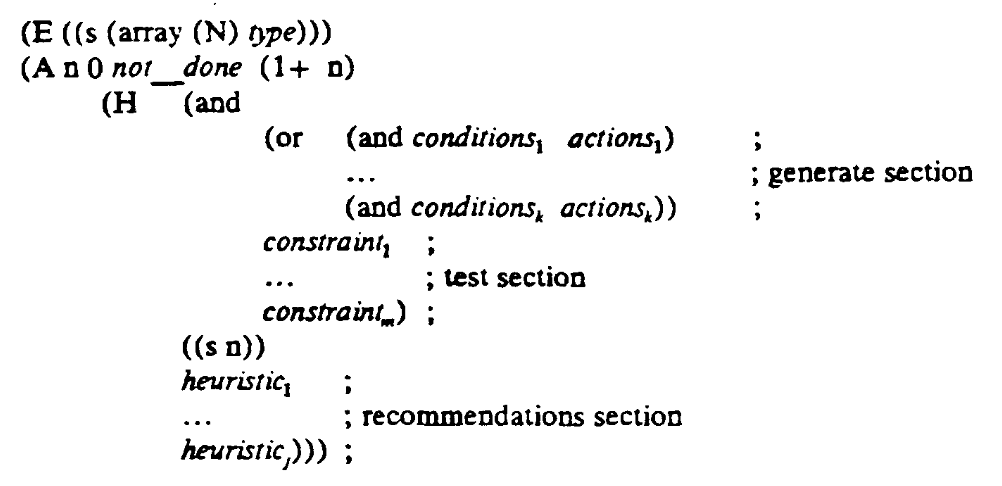
\includegraphics[width=.7\textwidth]{img/CHORAL_loop.png}
	}
	
	\drawat{8.5cm,4cm}{
		\begin{infobox}[6.5cm]{Example Rule \only<1>{1}\only<2>{2}\only<3>{3}\only<4>{4}}
			\only<1>{
				In the very first chord, one can start with either in the tonic (I) \textbf{or} the dominant(V) degree of the key. \citep[p.240]{CHORAL_report}
			}
			\only<2>{
				A pitch \textbf{cannot} occur both altered \textbf{and} unaltered in the same chord. \citep[p.238]{CHORAL_report}
			}
			\only<3>{
				\textbf{For} any voice v<soprano, the melodic span of the skeletal pitches of voice v from the beginning of the chorale up to \textbf{and} including the current pitch, \textbf{cannot} exceed a thirteenth. \citep[p.253]{CHORAL_report}
			}
			\only<4>{\scriptsize
			\textbf{If} the previous chord is the VI degree of a major key \textbf{or} the I degree of a minor key, \textbf{and} \textbf{(}the current chord is a major triad whose root is a major second below that of the previous chord, \textbf{or} the current chord is a minor triad whose root is a perfect fourth below that of the previous chord\textbf{)}, \textbf{then} a new key whose tonic is equal to the root of the current chord can be entered at degree I. \citep[p.245]{CHORAL_report}
			}
		\end{infobox}
	}
\end{frame}

\begin{frame}{III. \dimThreeTitle}{David Cope's EMI (data-driven)}
	
	\underline{Methodology} (informal):
	\begin{itemize}	
		\item[(1)] \textbf{deconstruction} (analyze and separate into parts)
		\item[(2)] \textbf{signatures} (commonality - retain that which signifies style) 
		\item[(3)] \textbf{compatibility} (recombinancy - recombine into new works)
		\item[\warnSign] Still: the concrete implementation relies on \emph{heuristics}
	\end{itemize}
	
	\medskip
	\begin{quote}
		\enquote{All the great books are constructed from recombinations of twenty-six letters. Similarly, most of the great works of Western art music exist as recombinations of twelve pitches. The secret lies \textbf{not} in the \textbf{invention of new letters} or notes but in the subtlety and \textbf{elegance} of their \textbf{recombination}.} - {\footnotesize David Cope (1996)}
		\\\hfill{\tiny(\url{artsites.ucsc.edu/faculty/cope/experiments.htm})}
	\end{quote}
	
	The dataset describes a composer's \emph{style} \citep{Cope96}\\
	\hfill\conclude~Albums: \enquote{Bach by Design}; \enquote{Virtual Mozart}; \enquote{Virtual Rachmaninov}
\end{frame}

\begin{frame}[t]{III. \dimThreeTitle}{Learning Methods (data-driven)}
	\parbox[c]{.49\textwidth}{
		\underline{Artificial neuron}
		\medskip

		\includegraphics[width=0.49\textwidth]{img/ArtificialNeuronModel_english.pdf}
		
		\[ o_j = \varphi \left( \theta_j + \sum_{i=1}^n w_{ij} x_{ij} \right) \]
	}
	\parbox[c]{.49\textwidth}{
		\vspace{.5cm}
		\underline{Neural network}
		\smallskip
		\\Multilayer perceptron (MLP)\\
		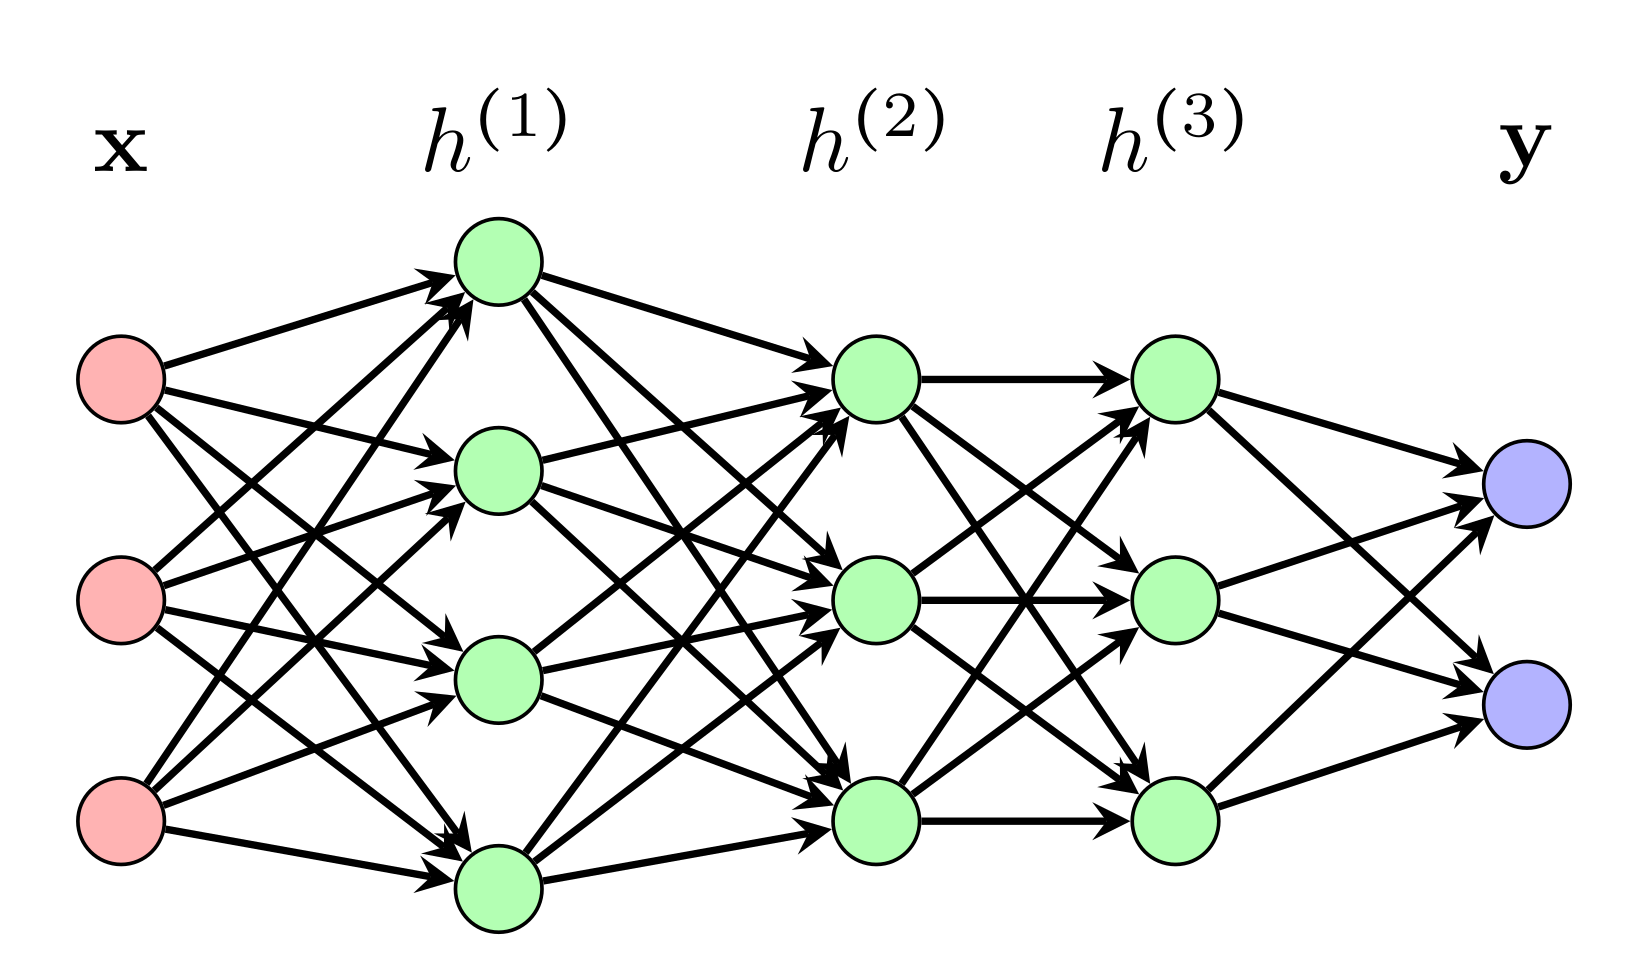
\includegraphics[width=0.49\textwidth]{img/MLP-Theorie.png}
		
		\raggedleft
		Learns features \emph{more or less} autonomously\\
		\smallskip
		\conclude~\emph{type of data} nearly \underline{irrelevant}
	}
\end{frame}

\begin{frame}{IV. \dimFourTitle}
	\attentionSign~So far: all examples with symbolic output\\
	
	\centering
	\begin{multicols}{3}
		(1) \underline{Score synthesis}
		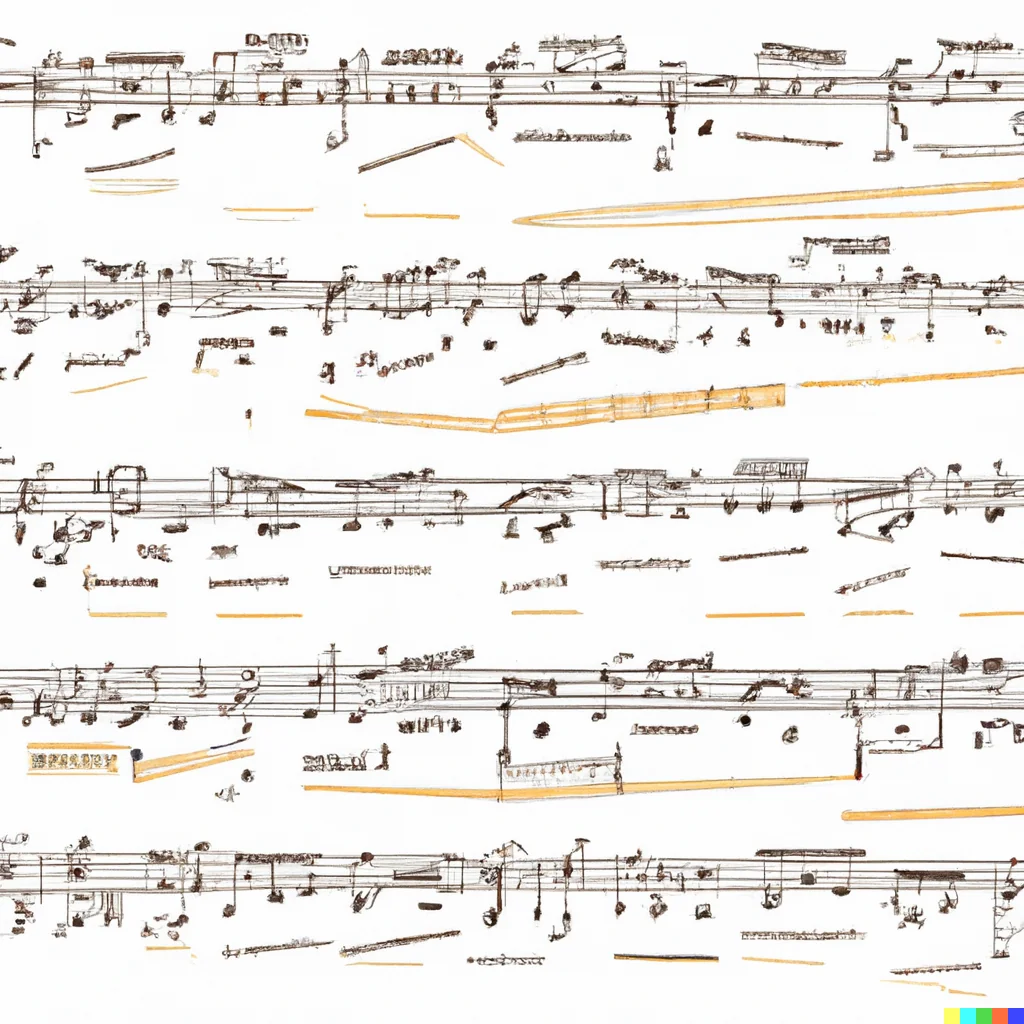
\includegraphics[width=.3\textwidth]{img/Dalle2-UndiscoveredMusicScoreByMozart.png}
		OpenAI Dall$\cdot$E\,2
	\columnbreak
	
		(2) \underline{Audio synthesis}
		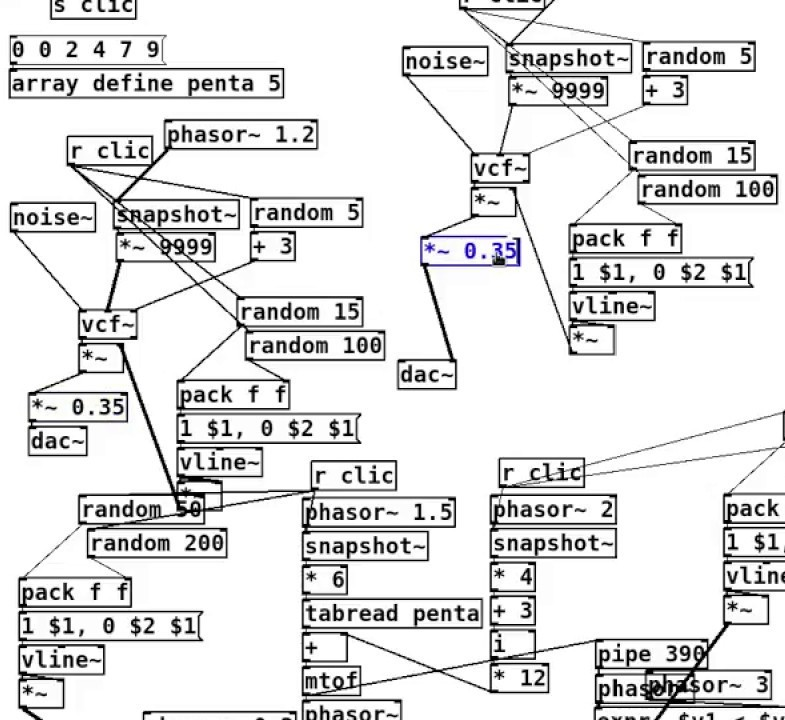
\includegraphics[width=.32\textwidth]{img/puredata.jpg}
		Pure Data\\
		
		{\small Visual Programming}
	\columnbreak
	
		(3) \underline{Waveform synthesis}
		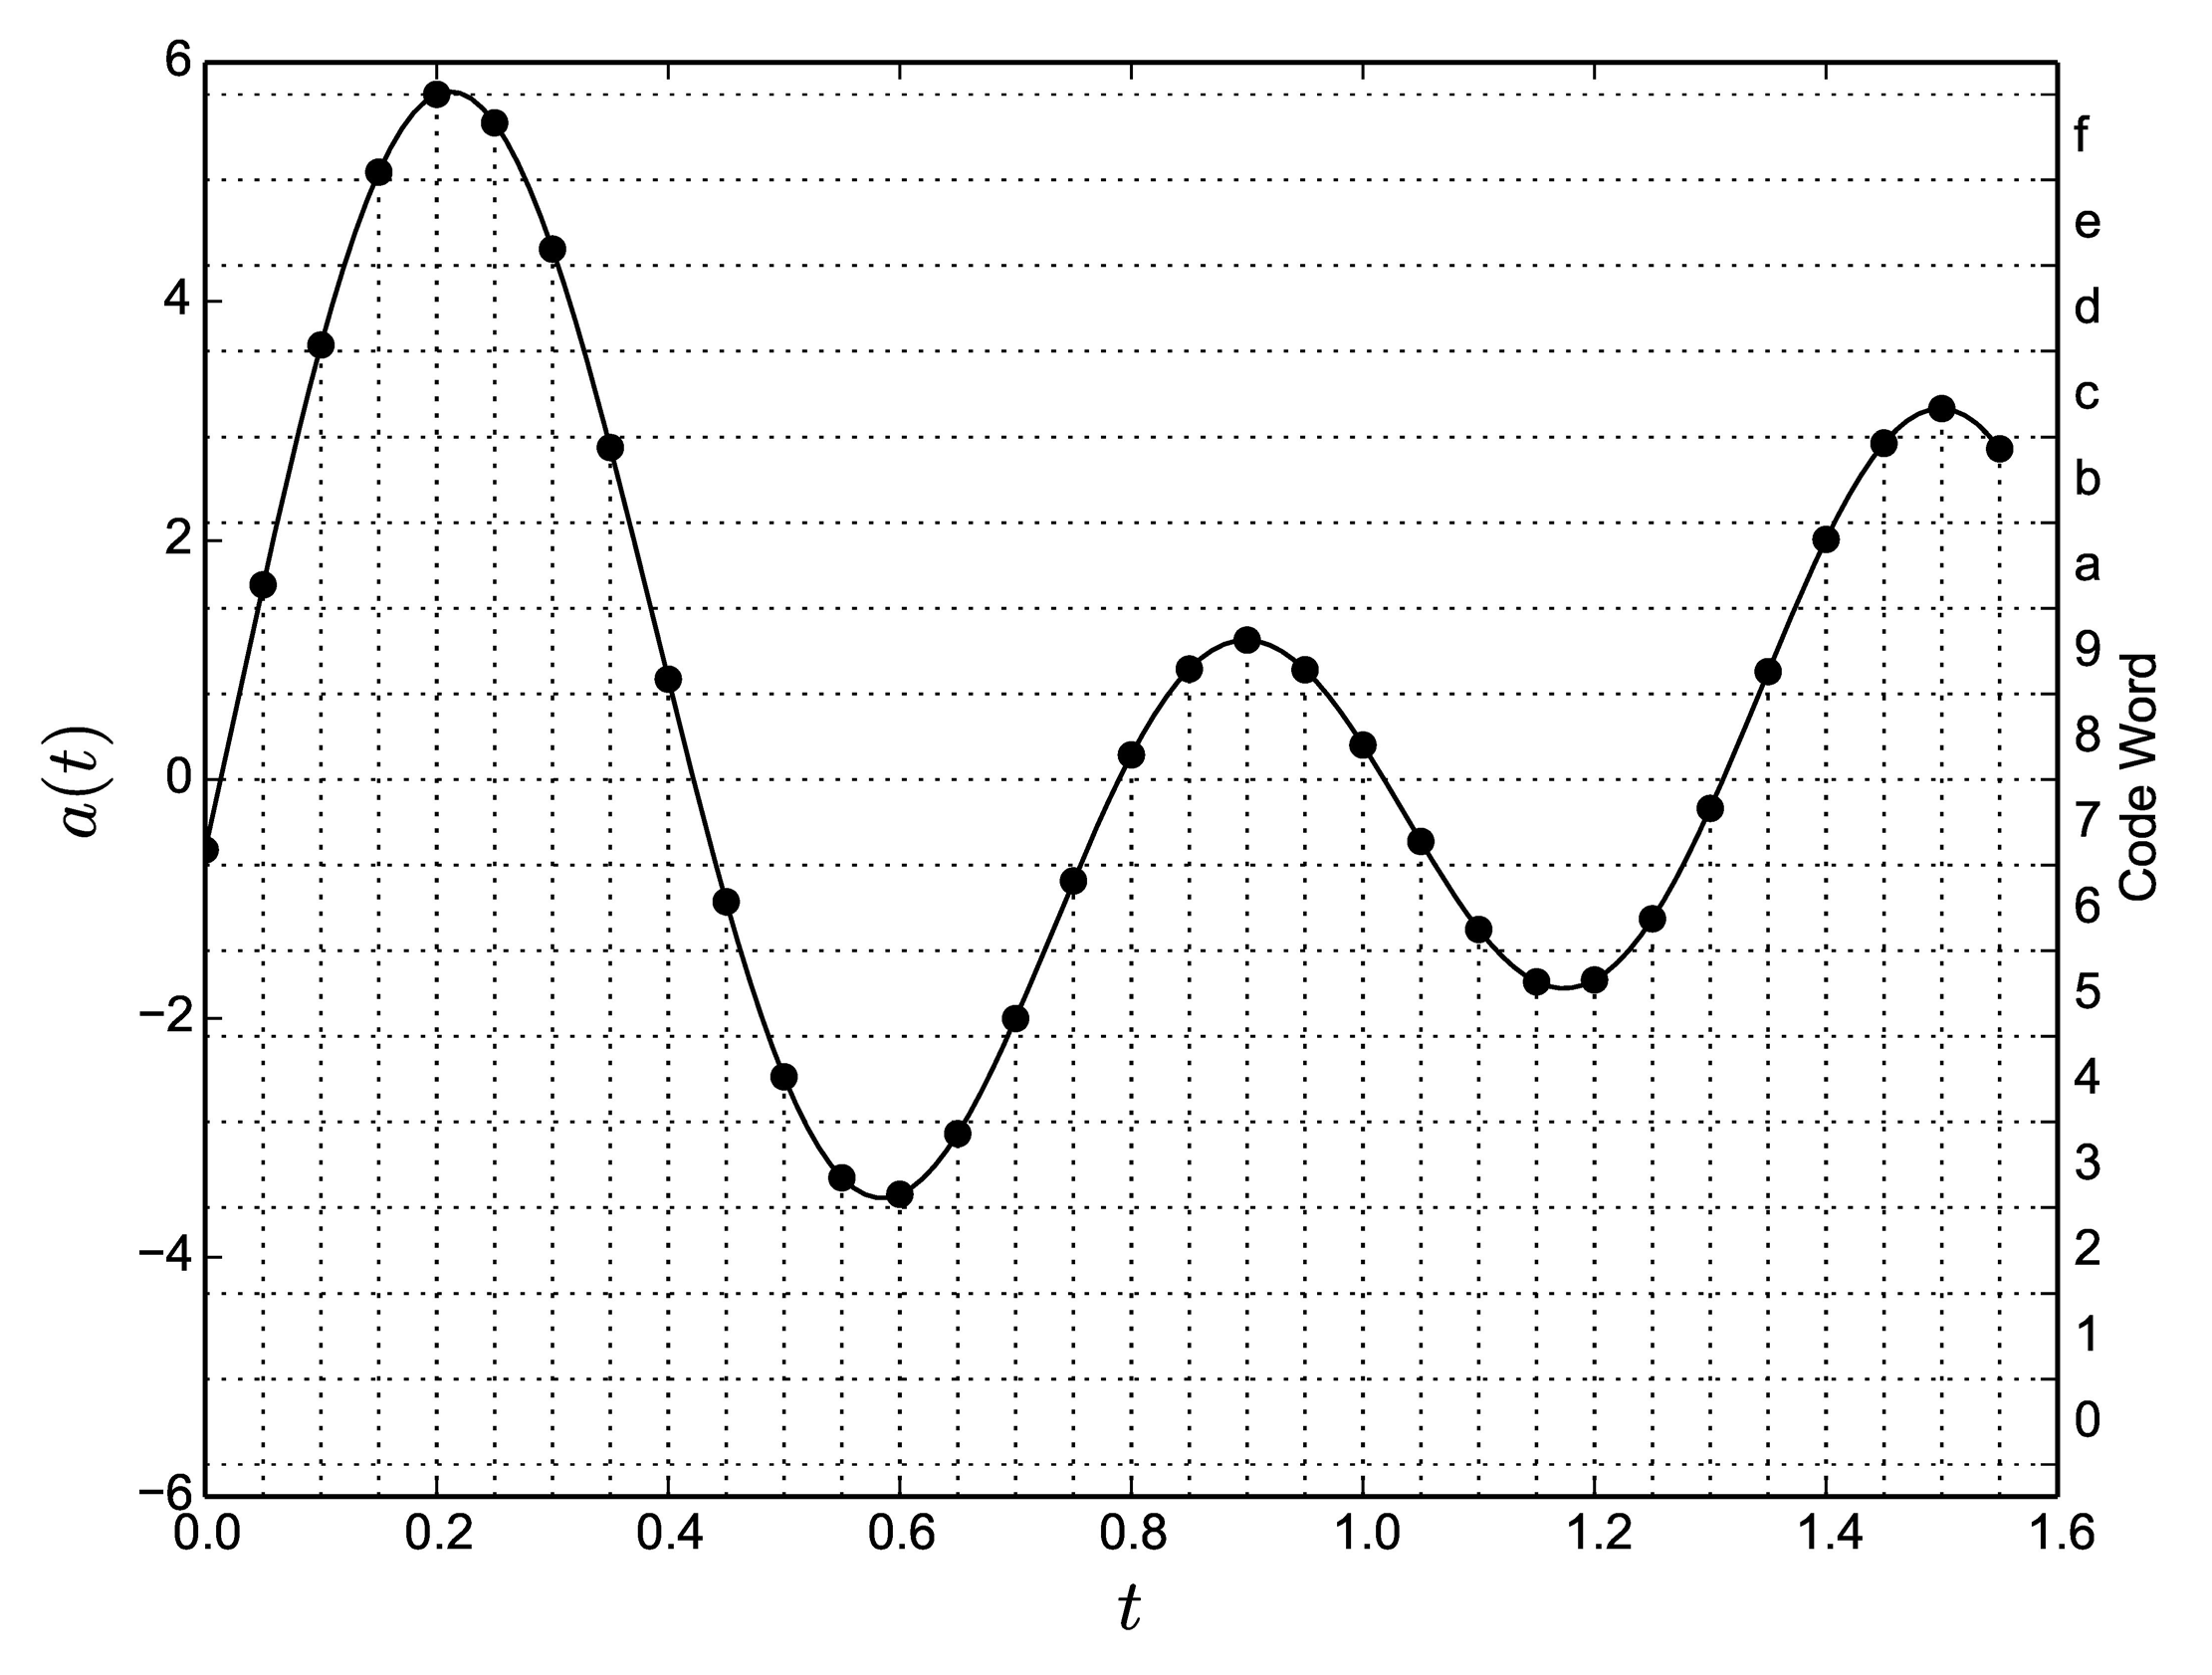
\includegraphics[width=.34\textwidth]{img/PCM_Waveform.png}
		OpenAI Jukebox\\
		
		{\small\url{openai.com/blog/jukebox/}}
	\end{multicols}
\end{frame}

\begin{frame}{Digitization of Audio Signals}
	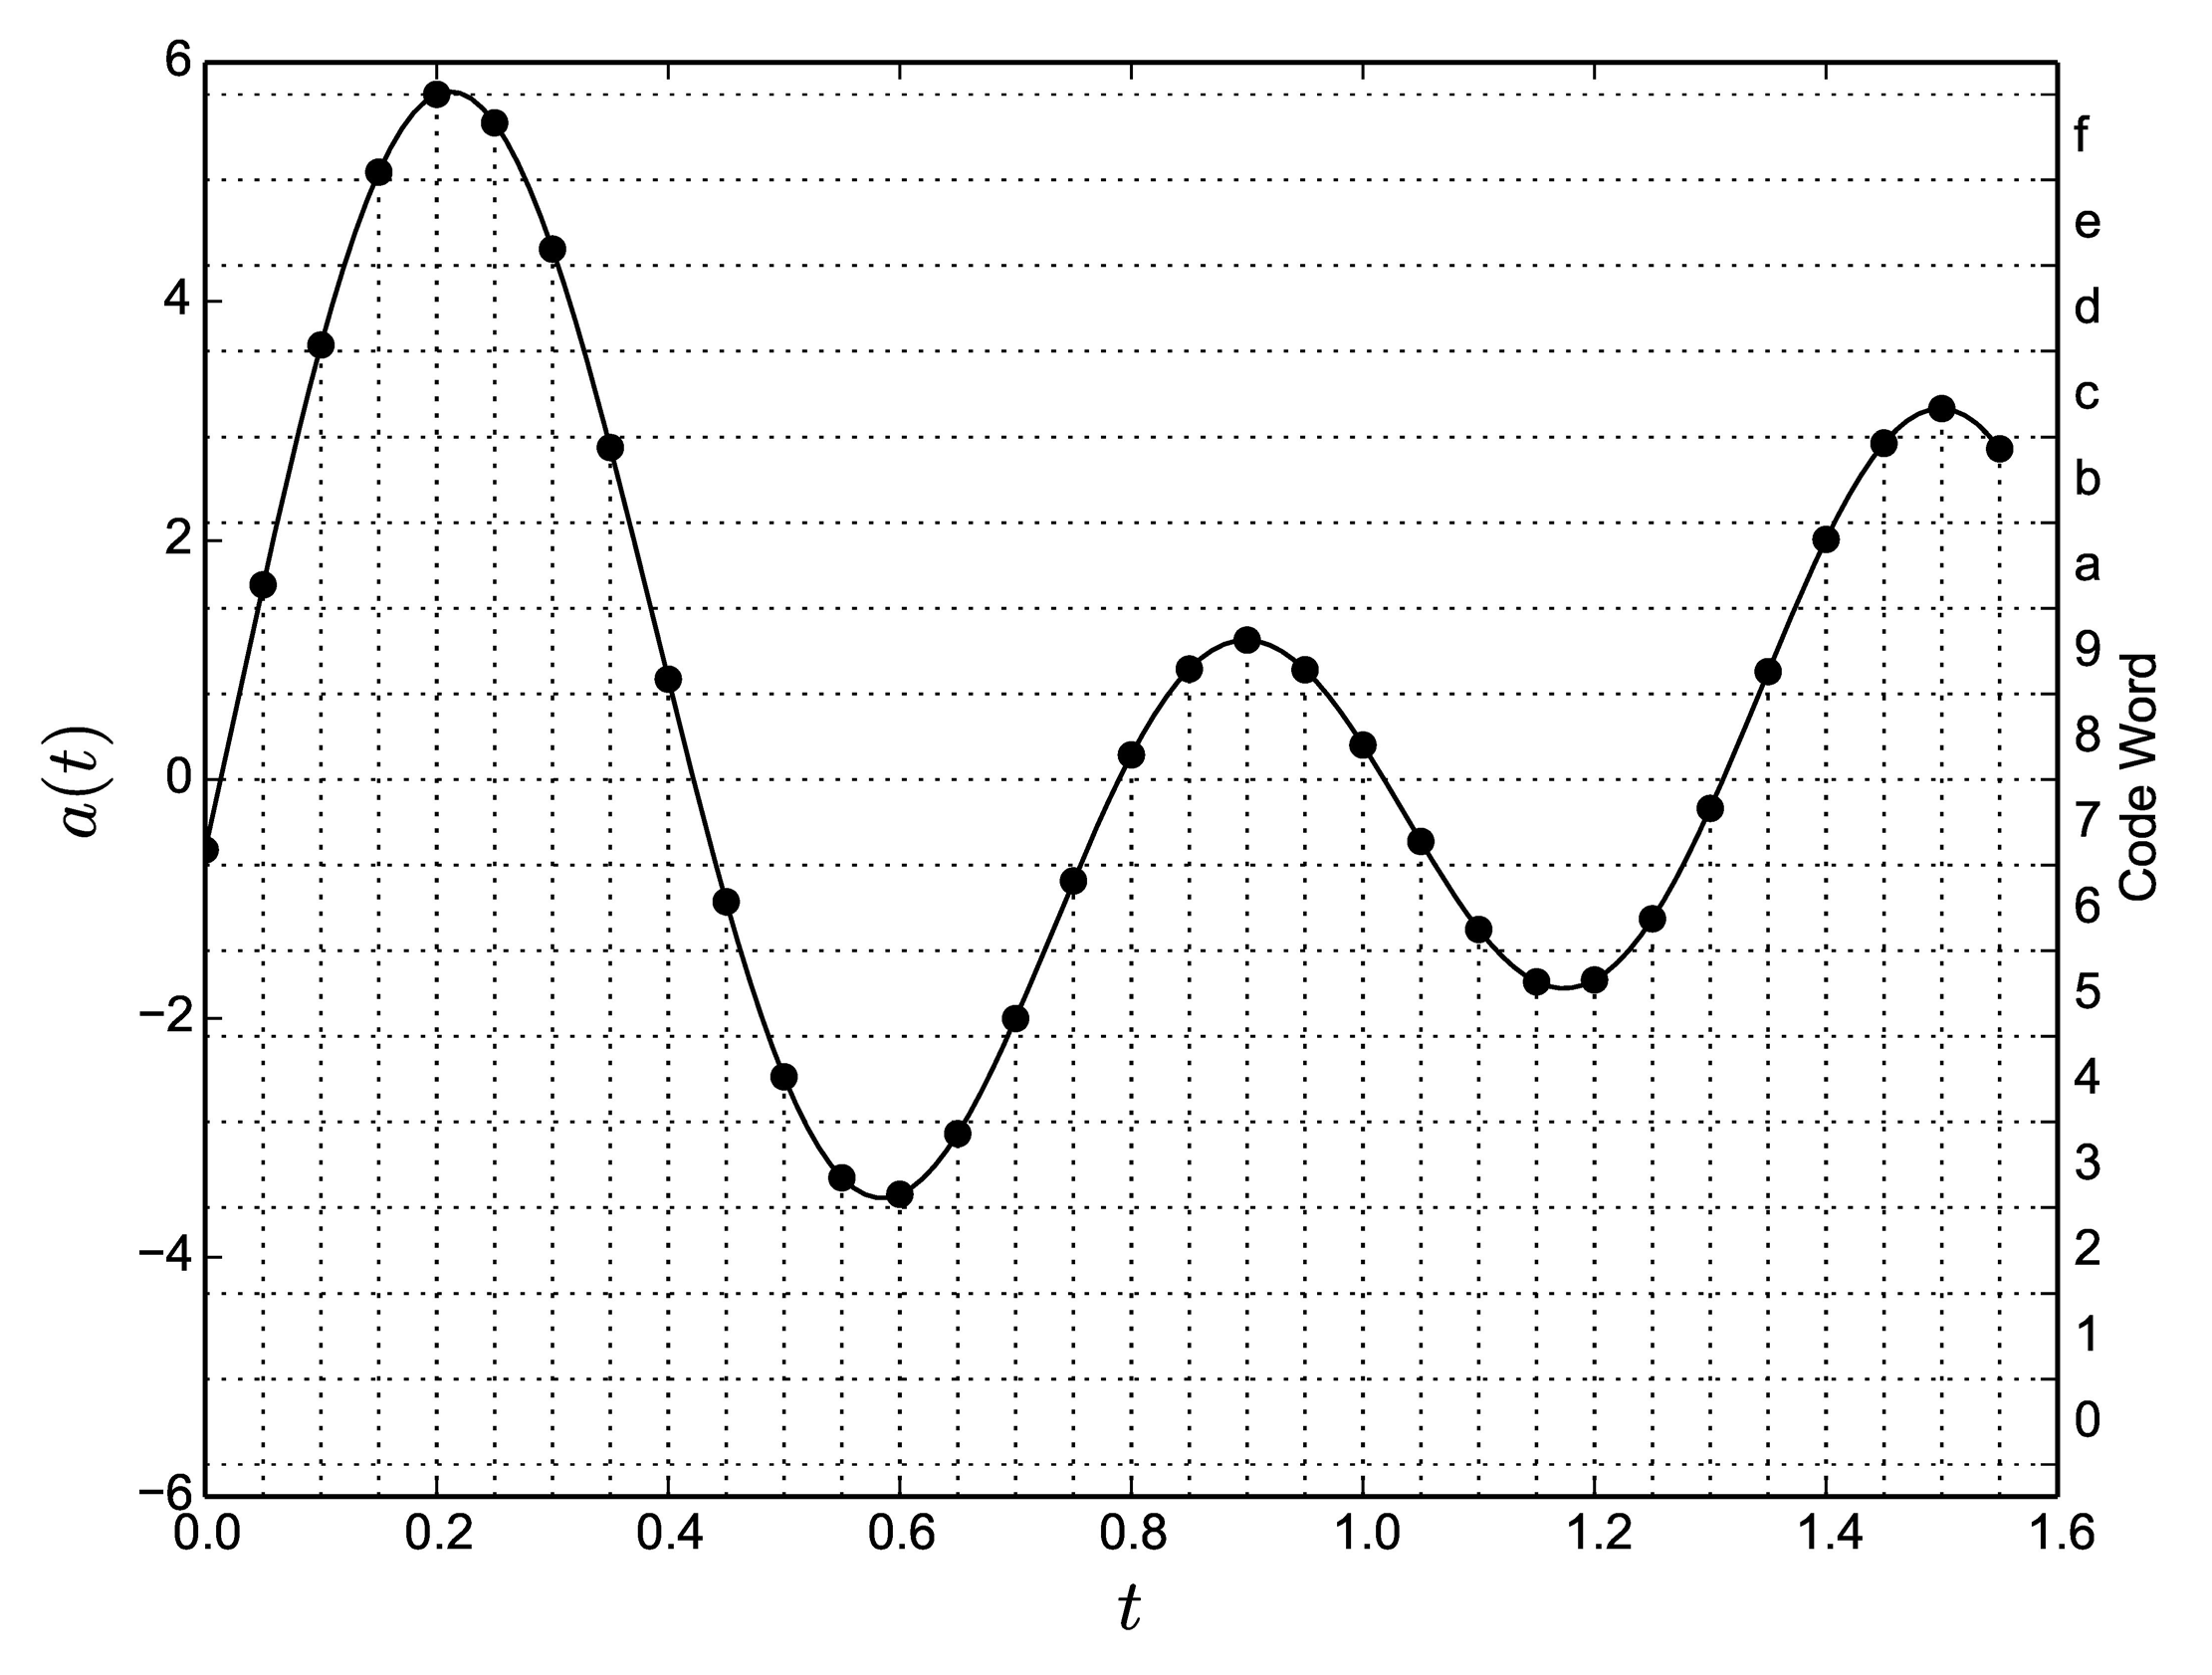
\includegraphics[height=.75\textheight]{img/PCM_Waveform.png}
	\drawat{105mm,15mm}{
		\begin{infobox}[50mm]{\small Sampling Theorem}
			\hyphenpenalty=10000 % temporarily disable hyphenation
			\footnotesize
			A signal band-limited to $f_{max}$ can be \emph{exactly} reconstructed from a sequence of equidistant samples if it was sampled at a frequency $f_s \geq 2 f_{max}$. 
		\end{infobox}
		
		\medskip
		\parbox{55mm}{
			\raggedright Solution space is huge\\
				\raggedleft(HiFi: 44.1\,kHz $\times$ 16\,bit)
			\begin{itemize}
				\item $\mu$-law companding\\
					\hfill(16\,bit $\to$ 8\,bit)
				\item neural audio codec (learned)
			\end{itemize}
		}
	}
	
\end{frame}

\begin{frame}{Fourier transform}
	\begin{center}
		\includegraphics[height=.55\textheight]{img/Fourier.pdf}
	\end{center}
	
	\vspace{-0.5cm}
	\conclude~more useful for \textbf{construction losses} then direct generation,\\
	~~~~~because amplitude+phase ($\in \mathbb{C}$) must be estimated (\emph{somehow})\\
	\bigskip
	
	\raggedleft
	Hearing-specific variant: \textbf{Mel Spectogram}\hspace{2.17cm}~\\
	Music-specific variant: \textbf{Constant-Q transform} (CQT)
\end{frame}

\HIDE{
\begin{frame}{Mel scale}
	\includegraphics[height=.45\textheight]{img/Mel-Hz_plot.pdf}	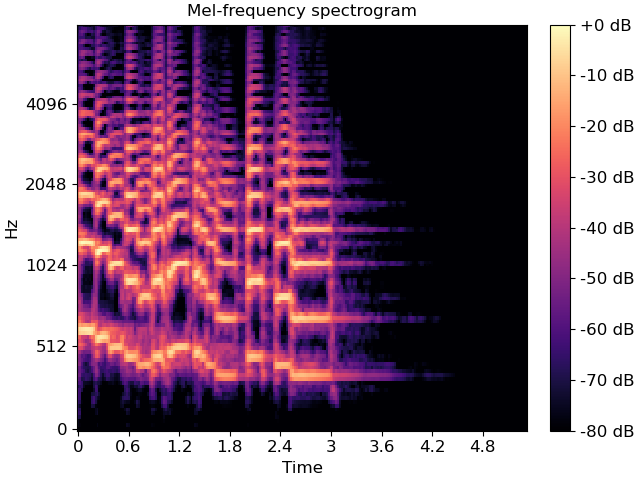
\includegraphics[height=.45\textheight]{img/librosa-feature-melspectrogram-1.png}
	
	$mel = 2595\log_{10}(1+\frac{f}{700})$
\end{frame}
}



\begin{frame}[t]{Symbolic Music Representation}{MIDI (1982)}
	\vspace{-0.75cm}
	\begin{columns}
		\begin{column}{0.6\textwidth}
			\emph{\textbf{M}usical \textbf{I}nstrument \textbf{D}igital \textbf{I}nterface}\\
			\small
			\mbox{Inter-communication protocol for musical control information}\\
			\smallskip
			
			Metaphor of \enquote{a piano being played}\\
			~~~~\textrightarrow~Stream of \texttt{NoteOn} {\footnotesize(key pressed)}\\
			~~~~~~~~~~and \texttt{NoteOff} events {\footnotesize(key released)}\\
			\bigskip
			
			\texttt{NoteOn} event:\\
			~~Pitch (\emph{key}) \& pressing force (\emph{velocity})\\
			\bigskip
			
			\warnSign~MIDI files carry \textbf{no sound}!\\
			\medskip
			
			\warnSign~events require timestamps (\emph{delta}),\\
			which makes \enquote{tokenization} non-trivial\\
			(current de facto standard: \texttt{REMI+})\\
			\medskip
			
			\textbf{\color{TUDoGreen}Pro}~~Huge MIDI corpora exist!
		\end{column}
		\begin{column}{0.4\textwidth}
			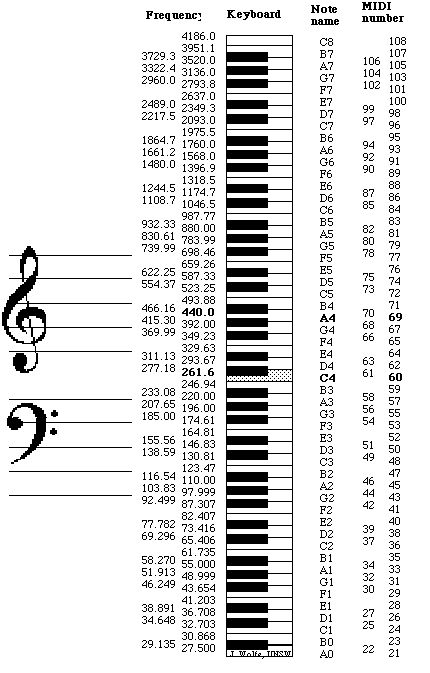
\includegraphics[width=0.9\textwidth]{img/MIDI-numbers.jpg}
		\end{column}
	\end{columns}
\end{frame}

\HIDE{
\begin{frame}[t,fragile]{Symbolic Music Representations}{various}
	{\large MusicXML}
	
	\begin{columns}
		\begin{column}{.5\textwidth}
			Header:
			\scriptsize
			\begin{verbatim}
<?xml version="1.0" encoding="UTF-8" standalone="no"?>
<!DOCTYPE score-partwise PUBLIC
"-//Recordare//DTD MusicXML 4.0 Partwise//EN"
"http://www.musicxml.org/dtds/partwise.dtd">
			\end{verbatim}
			~~~~~~~~~~\includegraphics[width=.6\textwidth]{img/MusicXML_C_Whole_Note.pdf}
			~~~~~ \raisebox{0.8cm}{\Large\textrightarrow}
			
			\small
			\underline{Caution}: symbolic representations are strong simplifications of the actual musical object!
		\end{column}
		\begin{column}{.3\textwidth}
			\vspace{-1.5cm}\tiny
			\begin{verbatim}
<score-partwise version="4.0">
	<part-list>
		<score-part id="P1">
			<part-name>Music</part-name>
		</score-part>
	</part-list>
	<part id="P1">
		<measure number="1">
			<attributes>
				<divisions>1</divisions>
				<key>
					<fifths>0</fifths>
				</key>
				<time>
					<beats>4</beats>
					<beat-type>4</beat-type>
				</time>
				<clef>
					<sign>G</sign>
					<line>2</line>
				</clef>
			</attributes>
			<note>
				<pitch>
					<step>C</step>
					<octave>4</octave>
				</pitch>
				<duration>4</duration>
				<type>whole</type>
			</note>
		</measure>
	</part>
</score-partwise>
			\end{verbatim}
		\end{column}
	\end{columns}
\end{frame}
}

\begin{frame}[fragile]{Symbolic Music Representations}
	\begin{figure}[t]
		\centering
			\begin{subfigure}[b]{0.25\textwidth}
				\centering
				\newdimen{\bwvh}\setlength{\bwvh}{375pt}
				\newdimen{\bwvw}\setlength{\bwvw}{830pt}
				\raisebox{0cm}{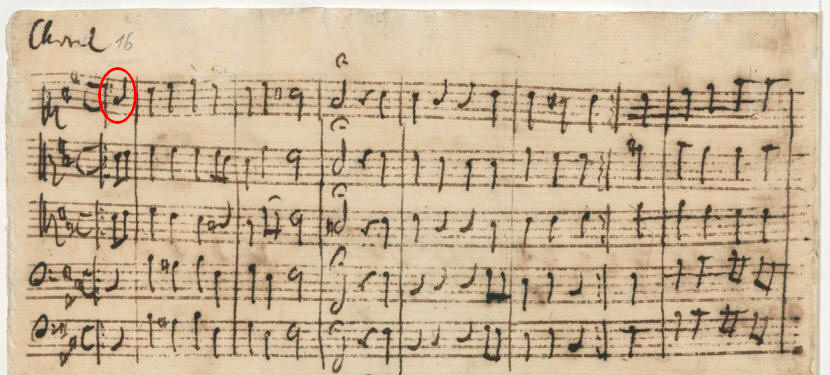
\includegraphics[width=.2\bwvw,height=.2\bwvh]{img/symb_reps//bwv84_choral_autograph_crop_marked.png}}
				\caption{hand-written\label{fig:bach-handschriftlich}}
			\end{subfigure}
			\begin{subfigure}[b]{0.25\textwidth}
				\centering
				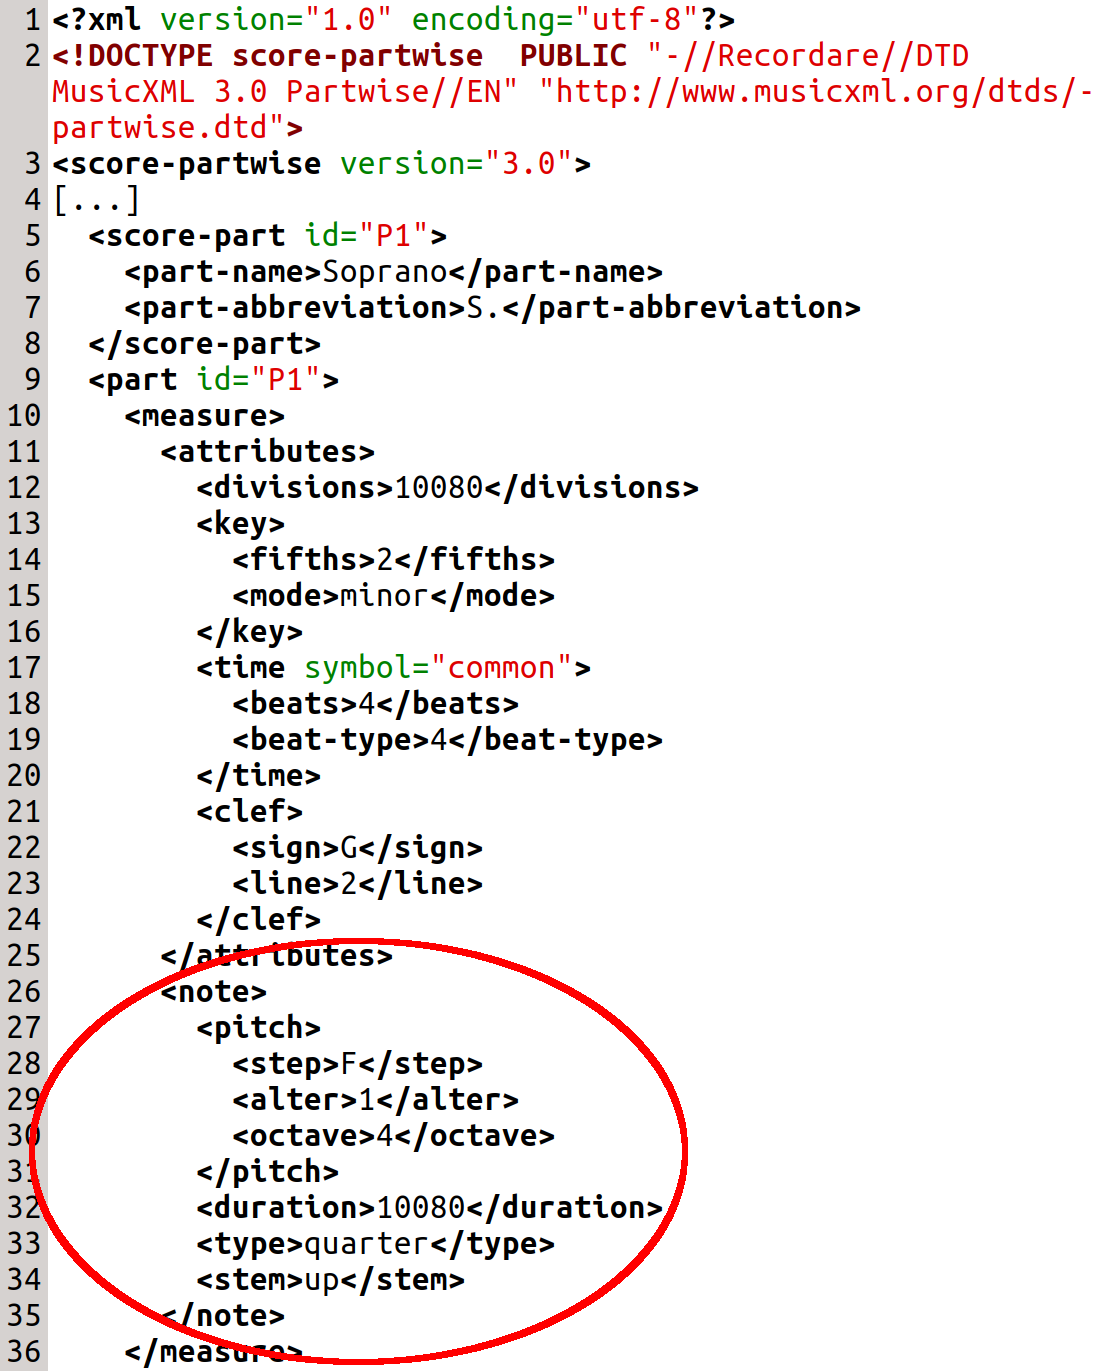
\includegraphics[height=5cm]{img/symb_reps/musicxml_marked.png}
				\caption{MusicXML\label{fig:bach-musicXML}}
			\end{subfigure}
			\begin{subfigure}[b]{0.25\textwidth}
				\centering
				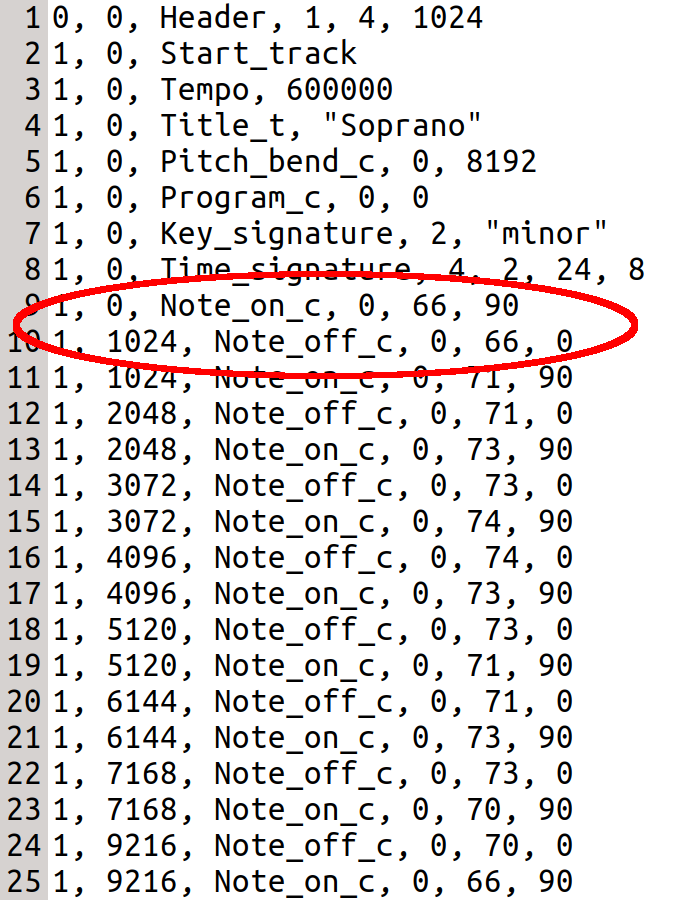
\includegraphics[height=5cm]{img/symb_reps/midicsv_marked.png}
				\caption{\texttt{midicsv}\label{fig:bach-MIDI}}
			\end{subfigure}
			\begin{subfigure}[b]{0.2\textwidth}
				\centering
				\includegraphics[height=5cm]{img/symb_reps/pianoroll-plot_marked.pdf}
				\caption{Pianoroll\label{fig:bach-pianoroll}}
			\end{subfigure}
		\label{fig:bach-notationen}
	\end{figure}
\end{frame}


\begin{frame}{V. \dimFiveTitle}{Overview with Examples}
	\centering	
	\begin{tikzpicture}[auto]
		\draw [<->, ultra thick] (0,0) node[anchor=north west,xshift=-1cm] {\emph{constrained/manageable}} -- (12,1) node[below] {\emph{complex}};
		
		\node[draw] (A) at (.5,.7) {Composition aid};
		\node[draw] (B) at (3.75,1.1) {Style transfer};
		\node[draw] (C) at (7.1,1.35) {Domain Competence};
		\node[draw] (D) at (11,1.6) {Original Composition};
		
		\node[above=.2cm of A] {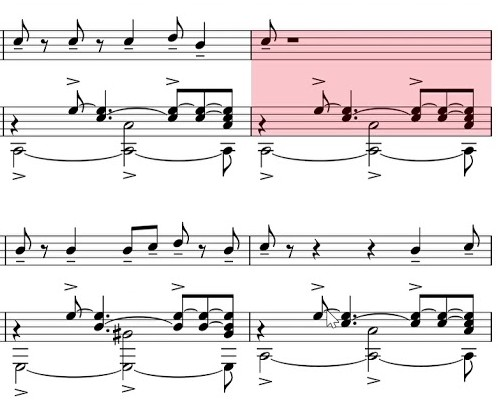
\includegraphics[width=3.2cm]{img/musescore_red.jpg}};
		\node[above=.2cm of B] {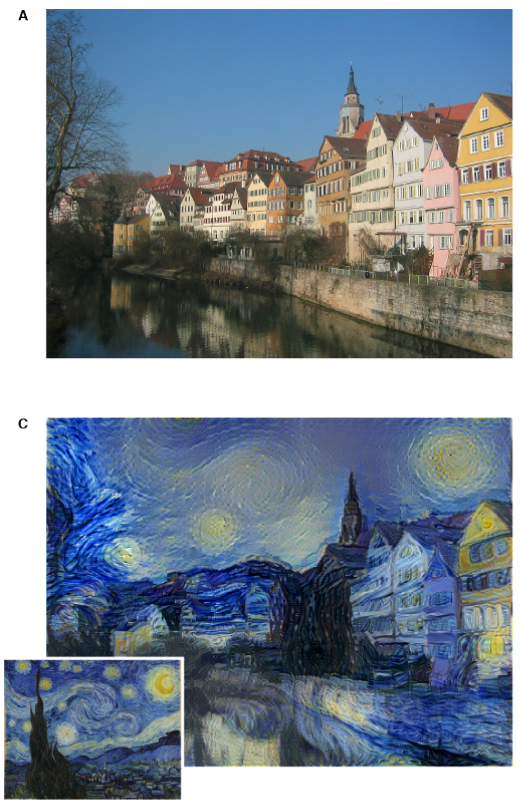
\includegraphics[width=2.6cm]{img/Stiltransfer.png}};
		\node[above=.2cm of C] {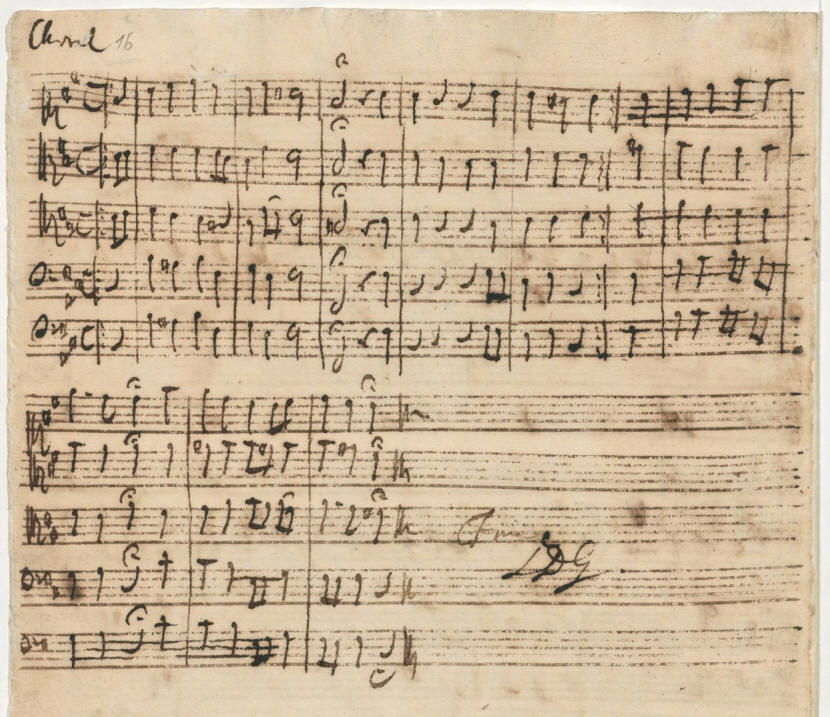
\includegraphics[width=3.5cm]{img/bwv84_choral_autograph.png}};
		\node[above=.2cm of D] {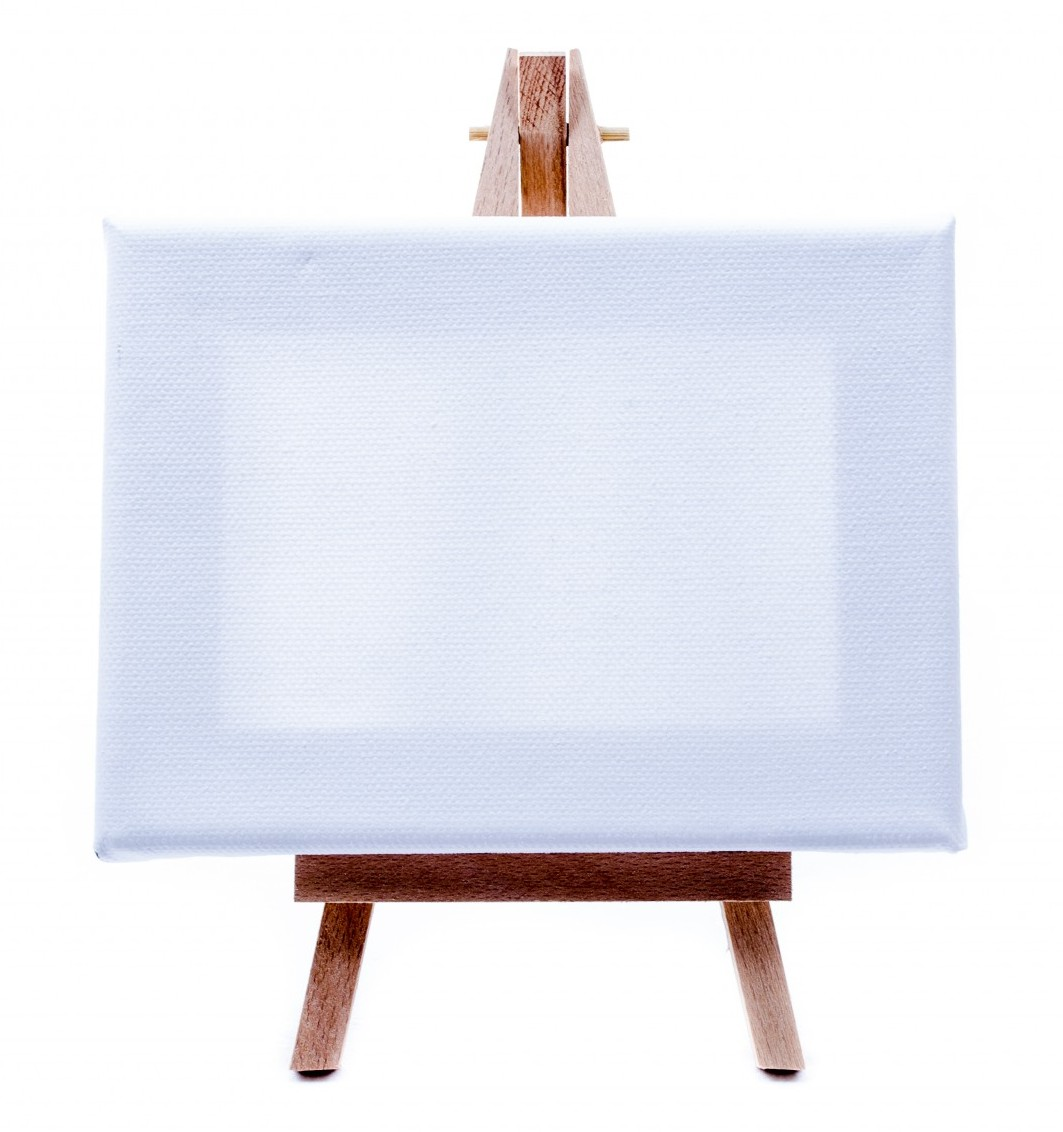
\includegraphics[width=2.8cm]{img/blank-canvas.jpg}};
	\end{tikzpicture}
\end{frame}

\begin{frame}{V. \dimFiveTitle}{DeepBach (2017)}
	\drawat{.72\textwidth,.6cm}{
		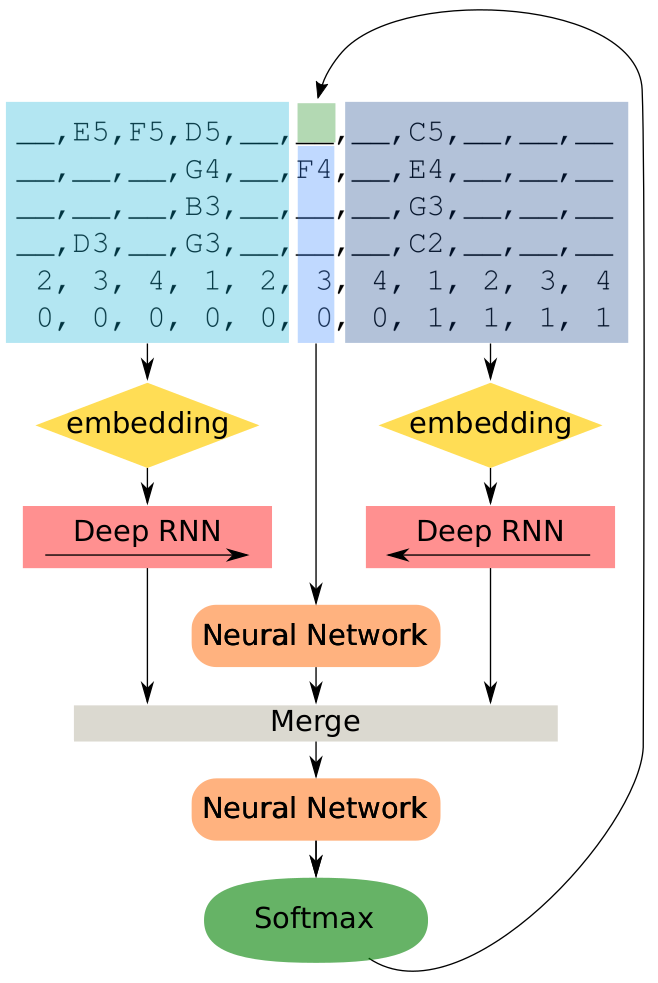
\includegraphics[height=.9\textheight]{img/DeepBach-Architektur.png}}
	\drawat{1.05\textwidth,.9\textheight}{\citep{DeepBach}}
	
	\parbox{.55\textwidth}{
		\begin{itemize}
			\item The model learns to predict exactly one entry (note) in the four-part texture
			\item Generation via\\\medskip
			~~~~~~\underline{\emph{Pseudo-Gibbs sampling}} {\footnotesize\citep{GibbsSampling}}
			\begin{enumerate}
				\medskip
				\item Input: length $L$, number of iterations $M$
				\item Initialize a four-part composition grid $K$ of length $L$\\with random values
				\item For $i=0$ to $M$ do:
				\begin{itemize}
					\item Choose a random entry $e$ in $K$
					\item Remove $e$
					\item Insert a new prediction for $e$ 
				\end{itemize} 
			\end{enumerate}
		\end{itemize}
	}

	\centering
	~~~~~~~~~~~~\audioplayer{audio/DeepBach-perfectfake01.mp3}
\end{frame}

\begin{frame}{V. \dimFiveTitle}{Original Composition: Iamus}
	\drawat{11.75cm,0.8cm}{\parbox{4cm}{\centering
		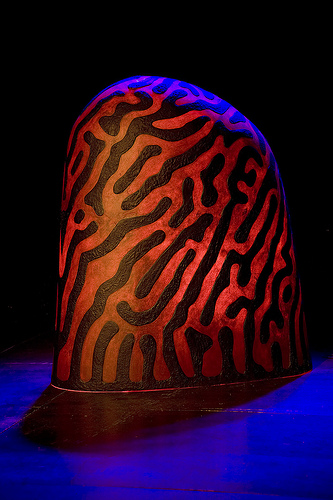
\includegraphics[width=3cm]{img/Iamus_server.jpg}
		Iamus computer cluster\\
		{\footnotesize(Universidad de Málaga)}
	}}
	
	\parbox{.8\textwidth}{
		\begin{itemize}
			\item Objective: new works of contemporary classical music
			\item Continuous development (motivic composition) based on an \textbf{evolutionary algorithm}
			\item Changes follow formal aesthetic criteria (\emph{formalism})\\
			\smallskip
			~~\warnSign~Once again, the criteria are \underline{heuristics}
			
			\medskip
			\item Storage: 70\,TB, RAM: 704\,GB
		\end{itemize}
		
		\bigskip\bigskip
		\centering
		\enquote{Hello World} (2011) \audioplayer{audio/Iamus_Hello_World.mp3}
	}
	
	\vfill
	\hfill \conclude~\textbf{International Computer Music Conference} (ICMC)
\end{frame}

\begin{frame}{V. \dimFiveTitle}{Evolutionary Algorithm (EA)}
	\begin{multicols}{2}
		\hspace{-1.2cm}
		\includegraphics[width=7.6cm]{img/EvoAlg_Scheme_english.pdf}
		
		\columnbreak
		\begin{itemize}\small
			\item[Initialization] Random or \enquote{clever}
			\item[Population] contains a set of \emph{individuals}\\
													\hfill(e.g., melodies)
			\item[Fitness] The individuals are scored \mbox{by a \emph{fitness function} (evaluation)}
			\item[Selection] \enquote{Survival of the fittest}
			\item[Parents] are recombined (e.g., \emph{crossover})
			\item[Mutation] Some individuals are randomly altered (at single points)
			\item[Offspring] form the next generation of the population
		\end{itemize}
	\end{multicols}
	
	\hfill \conclude~Conference on  \textbf{AI in Music, Sound, Art and Design} (EvoMUSART)
\end{frame}

\HIDE{
\begin{frame}{V. \dimFiveTitle}{EAR Drummer (2017)}
	\newcommand{\TAB}{\hspace{5mm}}
	\newcommand{\DS}{\displaystyle}
	\small
	\begin{columns}
		\begin{column}{.5\textwidth}
			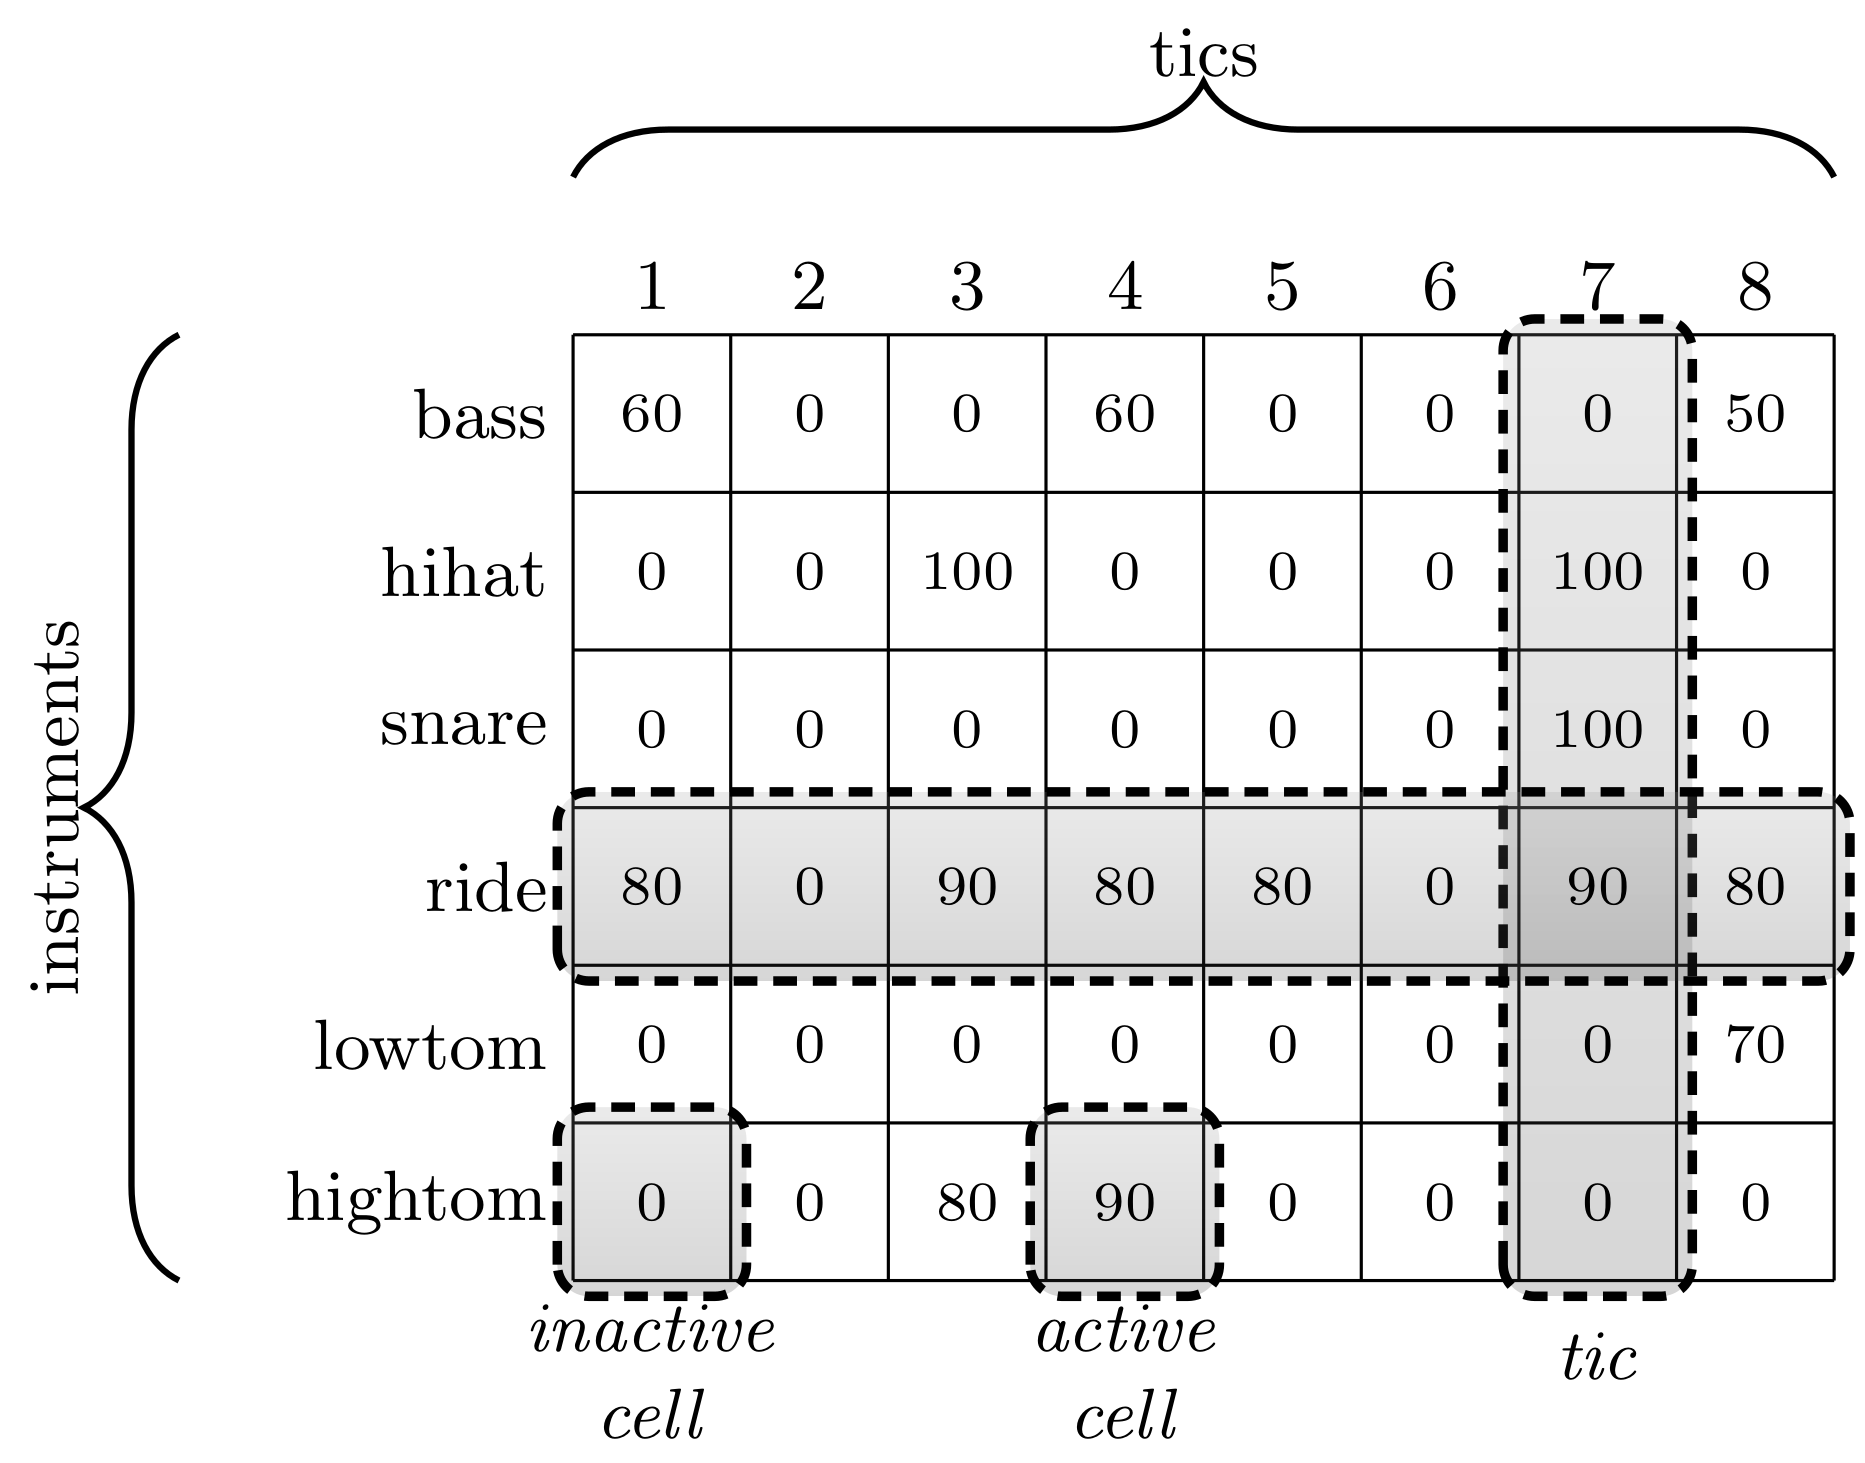
\includegraphics[width=\textwidth]{img/EarDrummer_genotype.png}
			Fitness is the degree of musical fit:\\
			\hspace{2.5cm} \fbox{\emph{human solo} $\overset{?}{=}$ \emph{drum pattern}}
		\end{column}
		\begin{column}{.6\textwidth}
			\underline{Implementation}: heuristic rules based on note statistics:
			\begin{enumerate}\scriptsize\setlength{\itemsep}{0pt}
				\item \textbf{length (leng)}: Duration of a note
				\item \textbf{keynumber (key)}: Mapping of a note to a key of the piano
				\item \textbf{volume (vol)}: Loudness of a note
				\item \textbf{interval (int)}: Interval between two consecutive notes
				\item \textbf{distance (dist)}: Duration between the start time of two consecutive notes
				\item \textbf{gap}:  Duration between end time of a note and start time of the consecutive note
			\end{enumerate}
			
			Three types of rules:
			\begin{itemize}\scriptsize\setlength{\itemsep}{0pt}\setlength{\itemindent}{.7cm}
				\item[Keep:] Preserve the initial pattern
				\item[Reaction:] Rate the \emph{drum pattern} according to a heuristic rule with respect to patterns in the note statistics
				\item[Random:] Noise produces more random behavior
			\end{itemize}
		\end{column}
	\end{columns}

	\scriptsize\raggedleft\vfill
	\textbf{Demo: }\url{https://github.com/FabianOstermann/EAR-Drummer}
\end{frame}
}

\begin{frame}[t]{VI. \dimSixTitle}{Human-In-The-Loop: GenJam (1994)}
	
	Al Biles modeled GenJam \citep{GenJam1994} as an artificial \textbf{music student}\\
	\hfill that learns the art of \textbf{jazz improvisation} over arbitrary chord progressions.
	
	\bigskip
	\centering
	\mbox{
		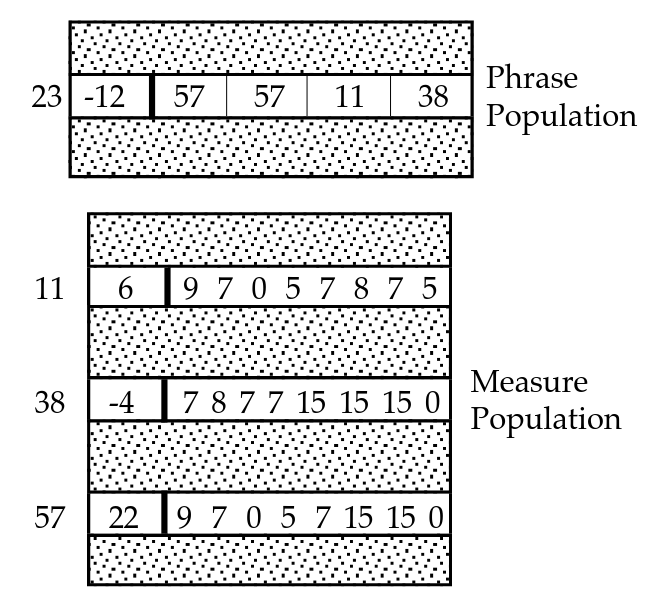
\includegraphics[width=.28\textwidth]{img/GenJam_PhraseMeasurePopulation.png}
		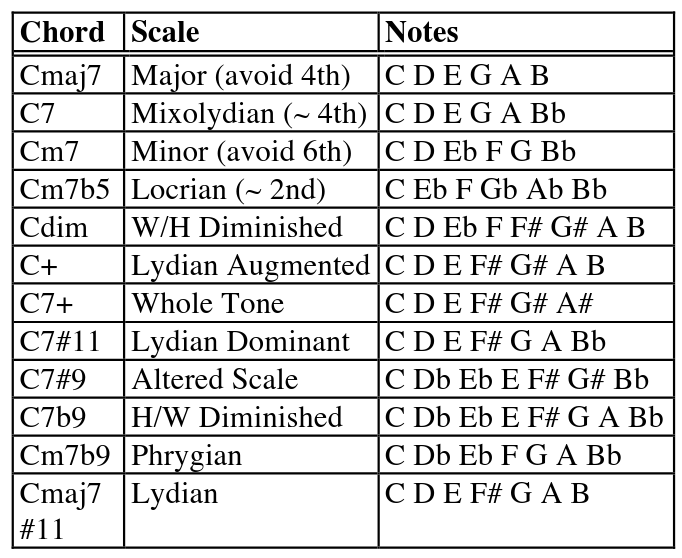
\includegraphics[width=.3\textwidth]{img/GenJam_ChordScaleMapping.png}
		~~~~~\parbox[b]{.4\textwidth}{
			\begin{itemize}
				\item[\ideaSign] Fitness values are determined \textbf{manually}!
				\medskip
				\item[\textbf{Pro}] The function acquires human qualities (cognition, intuition, innovation)
				\item[\textbf{Con}] Extremely laborious\\
						\hfill(humans are slow)
				\vspace{-.5cm}
			\end{itemize}
		}
	}
	
	{GenJam at New City Art, 2003} \audioplayer{audio/GenJam_at_New_City_Art,_2003_[ACT8Sy6tNZI].mp4}
\end{frame}

\begin{frame}{VI. \dimSixTitle}{Adaptive Video Game Music}
	Systems are typically simple so as not to \enquote{waste} computing resources\\
	Because: graphics \& physics of \enquote{blockbuster} games consume 50--90\% of computing time\\
	\medskip
	~~~\conclude~hence: music generation is often merely static or at best \textbf{rule-based}
	\medskip
	
	~~~~ Two basic techniques: {\footnotesize(can also be combined)}
	\medskip
	
	\drawat{4.5cm,5.8cm}{\mbox{\scriptsize\enquote{Synced Scores}}}
	~~\parbox[t]{.425\textwidth}{
		\mbox{(1) \underline{Horizontal Resequencing}}\\
		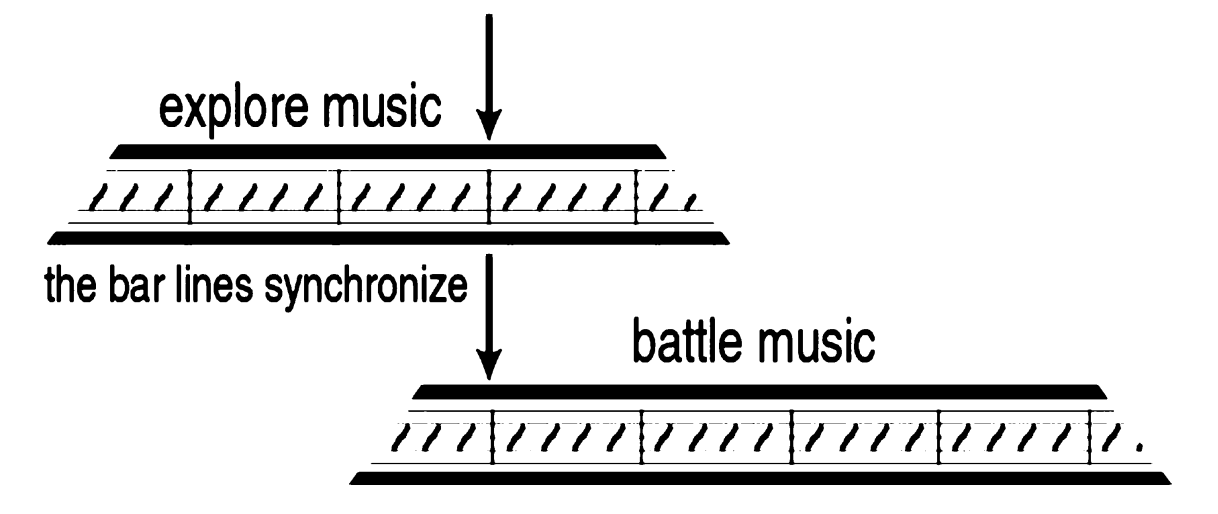
\includegraphics[width=0.4\textwidth]{img/GameMusic_SyncedScores.png}
	}
	\parbox[t]{.52\textwidth}{
		\mbox{(2) \underline{Vertical Remixing}}
			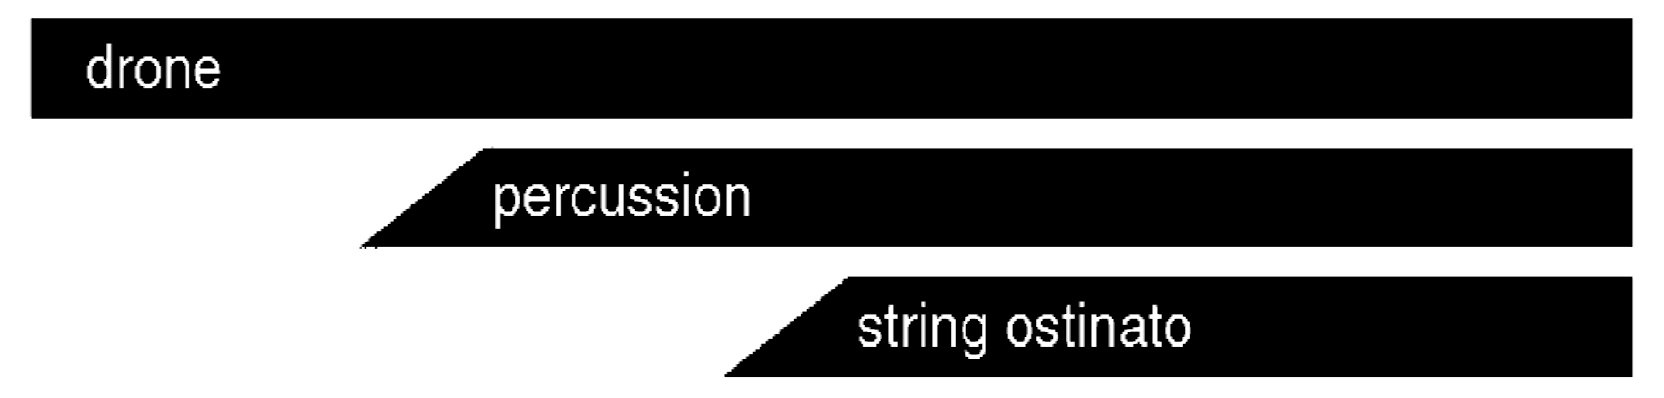
\includegraphics[width=0.55\textwidth]{img/GameMusic_VerticalRemixing.png}
	}
	
	\medskip
	\hfill\underline{Extensions}: Fade In/Out, Transitions, Score Branching, ...
\end{frame}

\begin{frame}{VI. \dimSixTitle}{iMuse in \emph{Monkey Island 2} (1991)}
	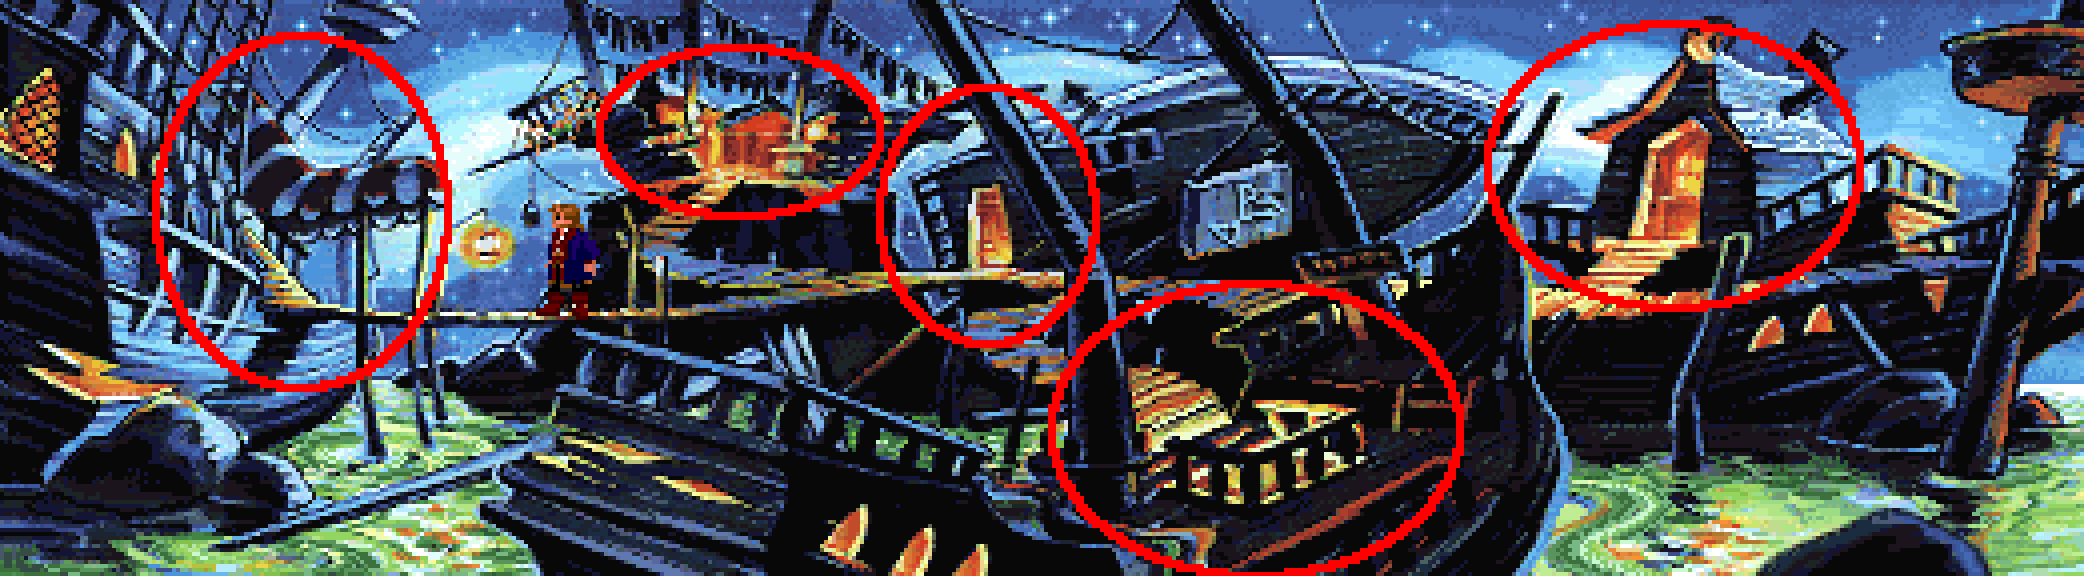
\includegraphics[width=0.8\textwidth]{img/woodtick_markered.png}\vspace{-.375\textheight}
	
	\hfill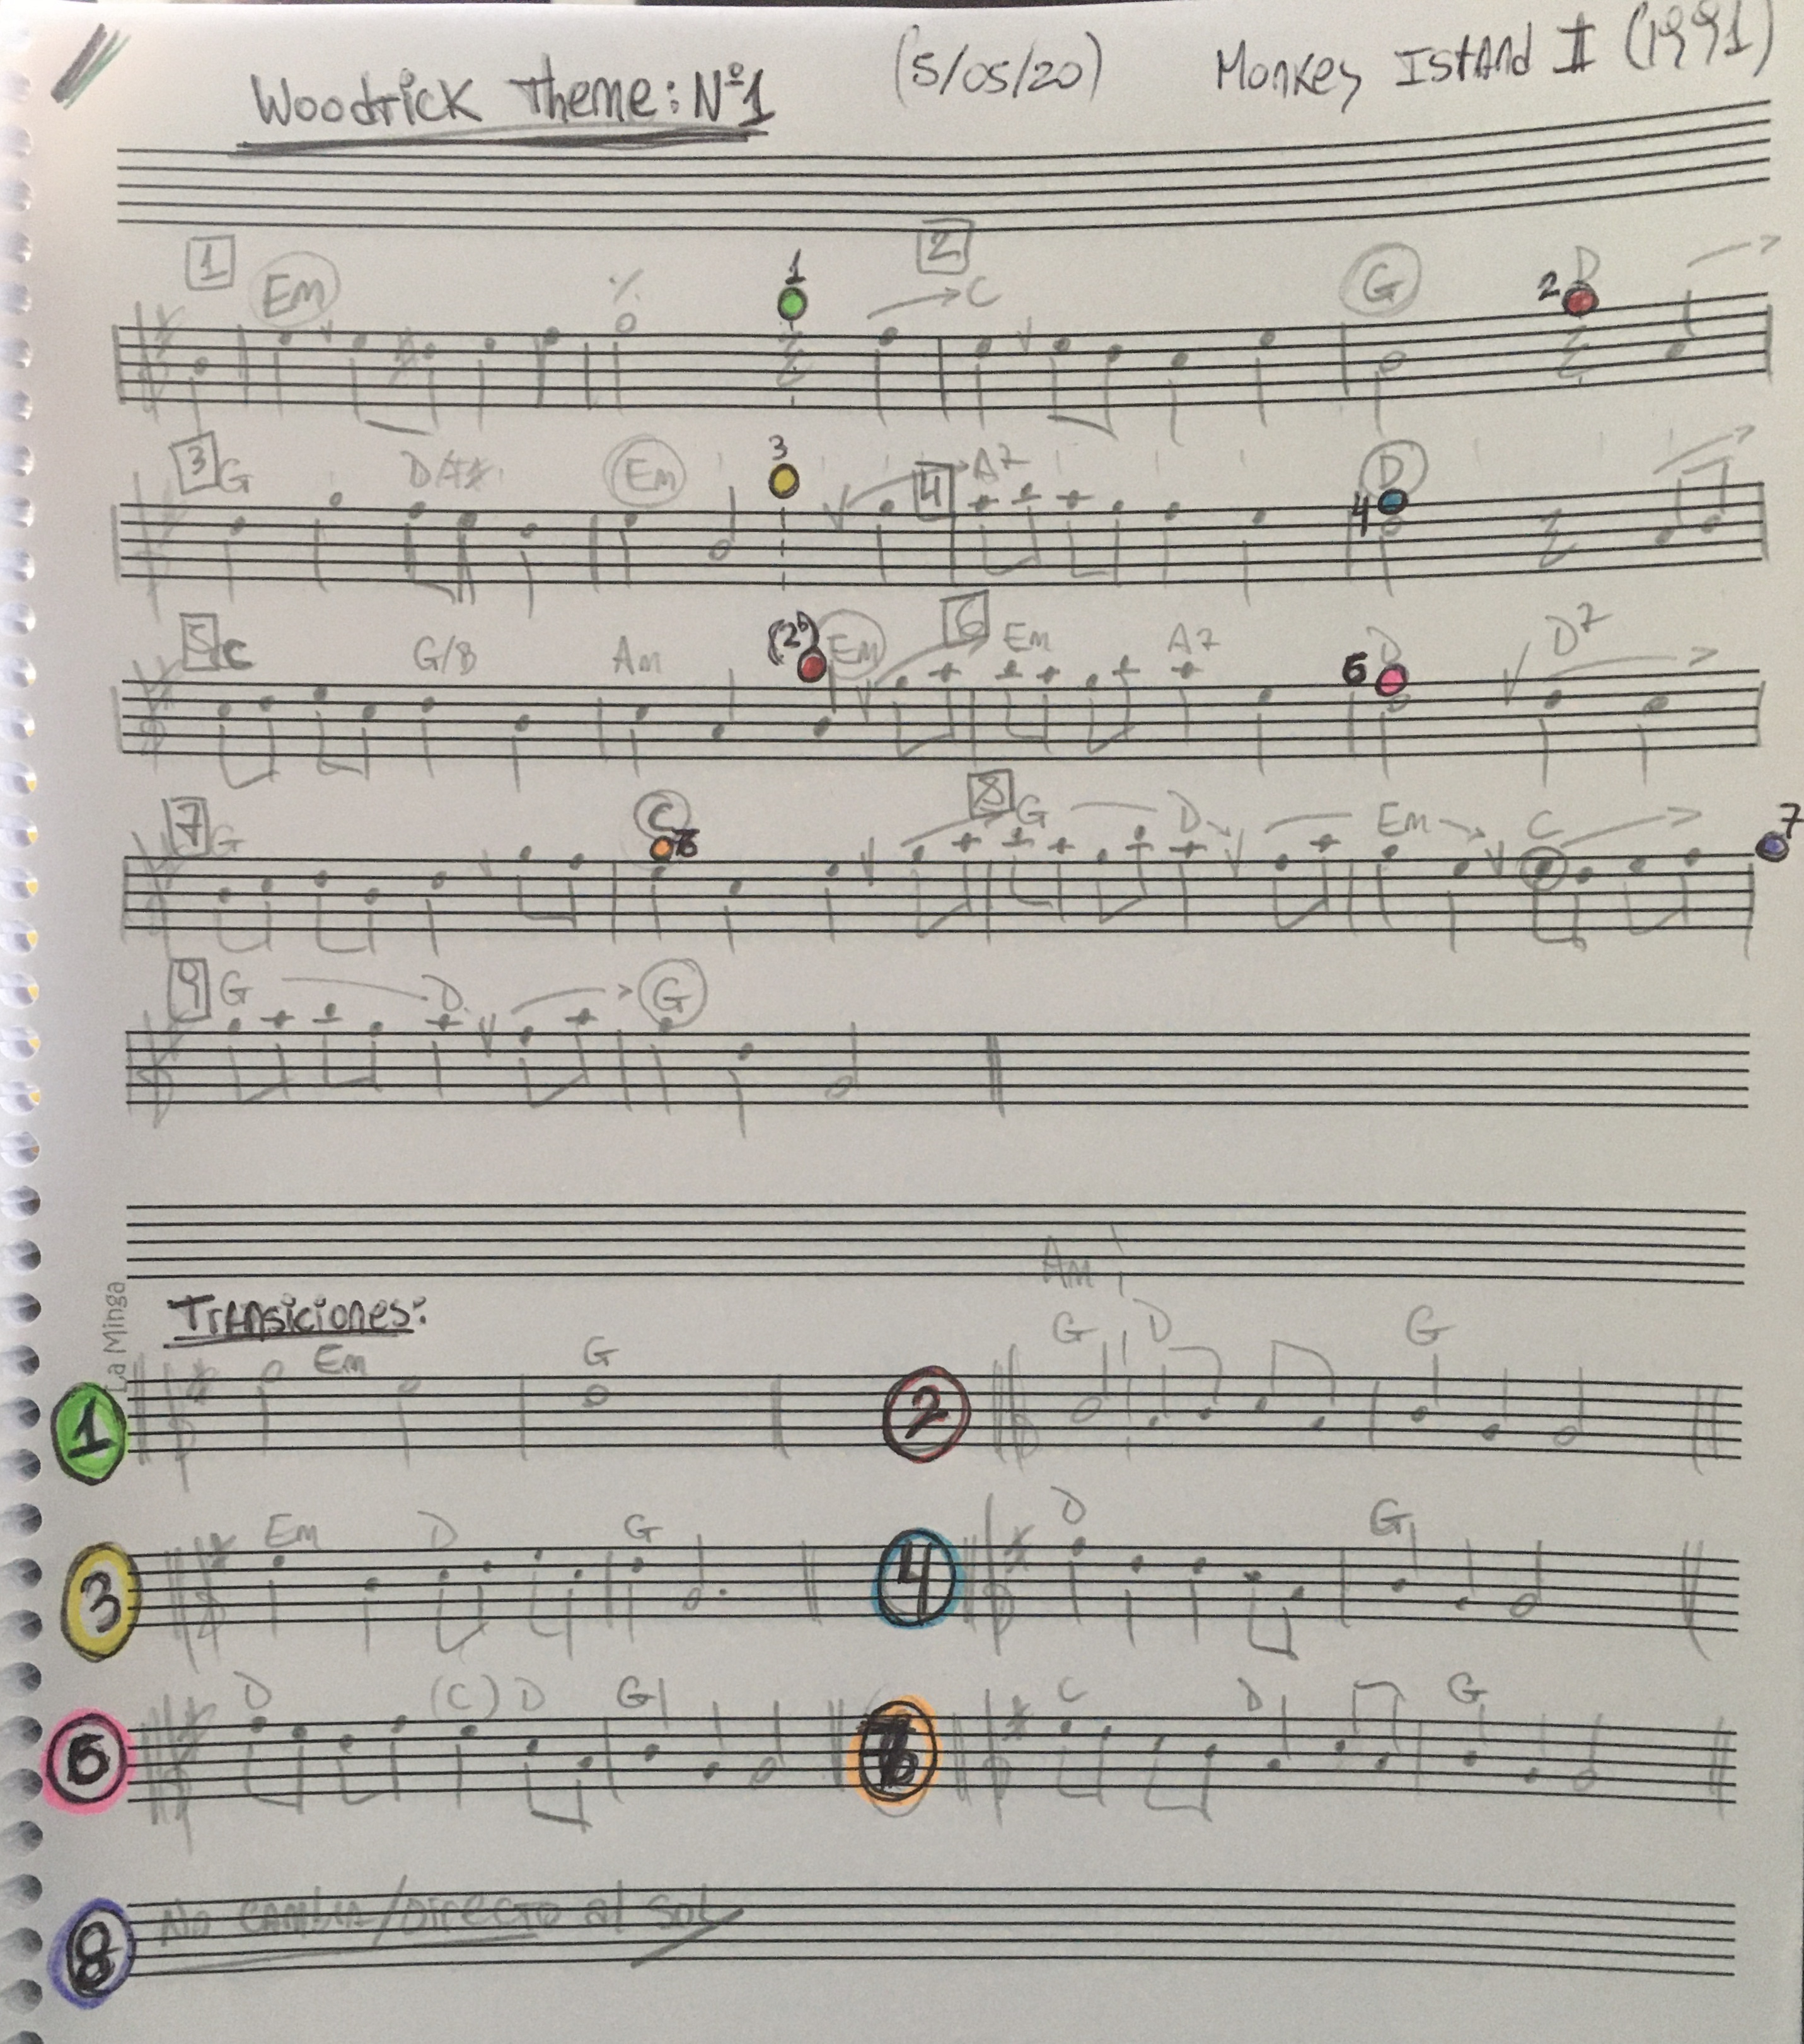
\includegraphics[height=.7\textheight]{img/woodtick_score.jpg}
	\vspace{-2cm}
	
	All transitions are composed manually\\
	\conclude~realistic effort only for \emph{blockbuster} productions\\
	
	\bigskip\small
	~~~~~~~~{Michael Z. Land \enquote{Woodtick Theme}} \audioplayer{audio/MI2_Wootick.mp4}
\end{frame}

\begin{frame}[t]{VI. \dimSixTitle}{Laptop Music, Algorave, Live Coding}

\Conclude~Comprehensibility of \emph{computer music} is a problem (for artists)\\
\hfill $\to$ as was for serial music and similar
\vspace{-.5cm}
\begin{center}
	\mbox{
		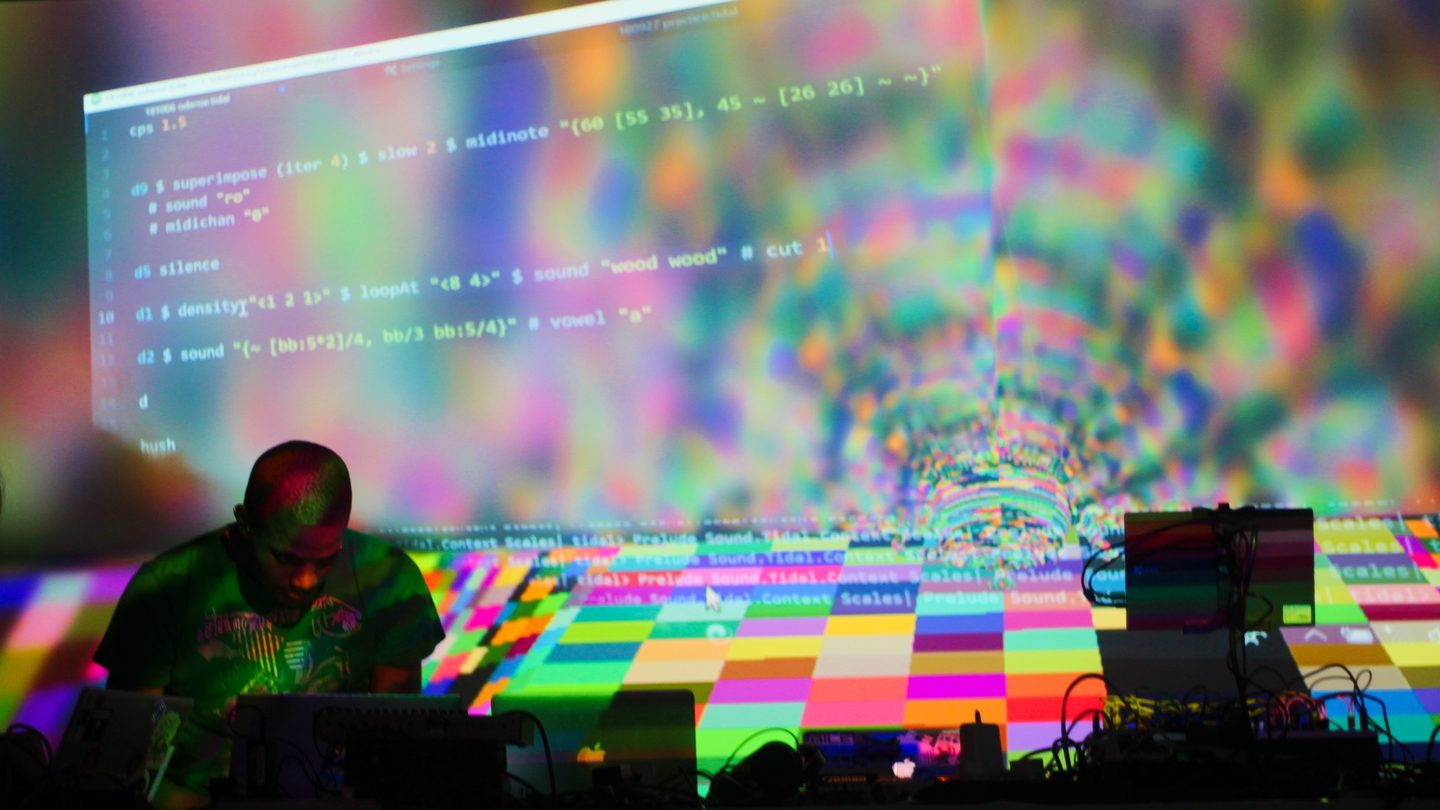
\includegraphics[width=.5\textwidth]{img/Algorave4_ByAntonioRoberts-1440x810.jpg}
		%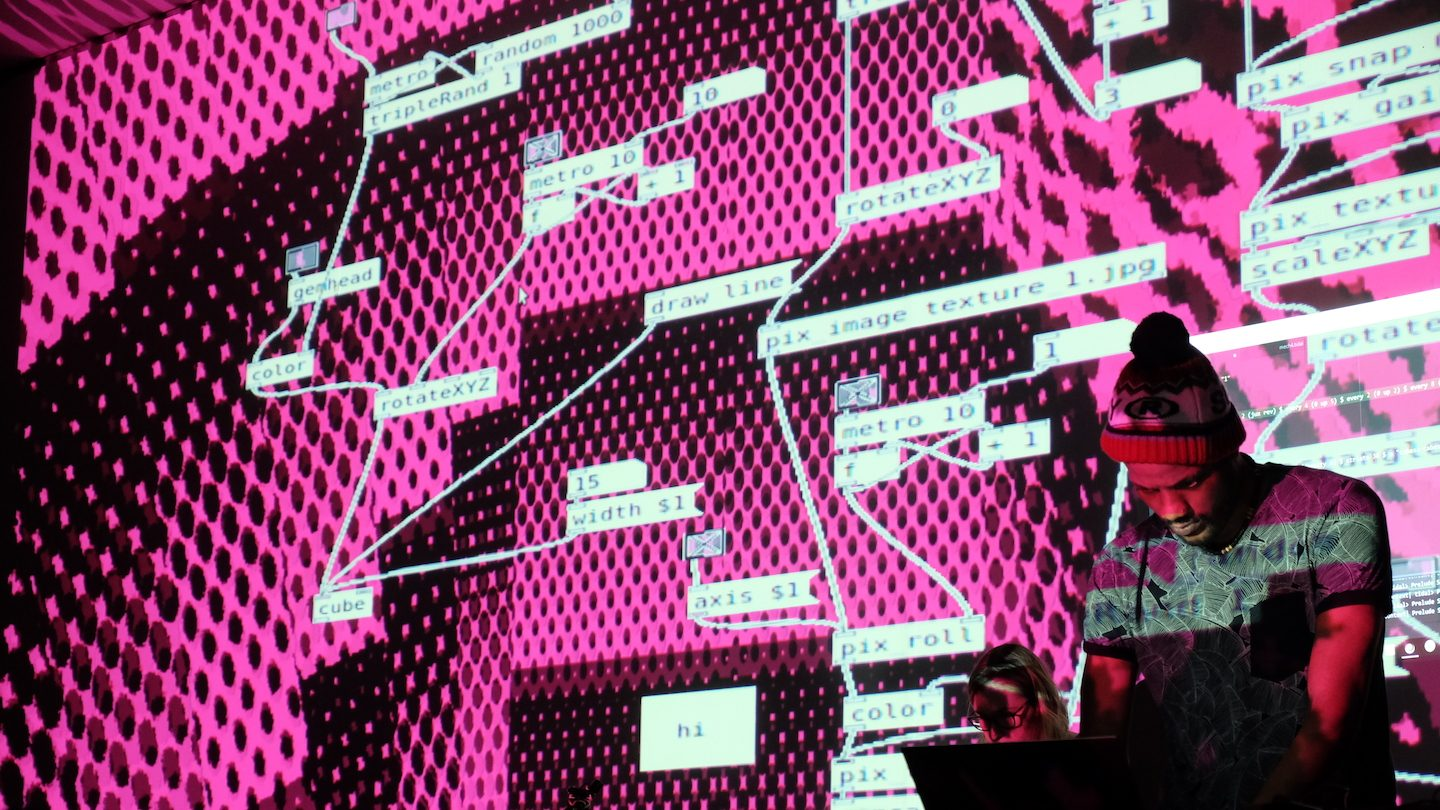
\includegraphics[width=.35\textwidth]{img/Algorave2_ByAntonioRoberts-1440x810.jpg}
		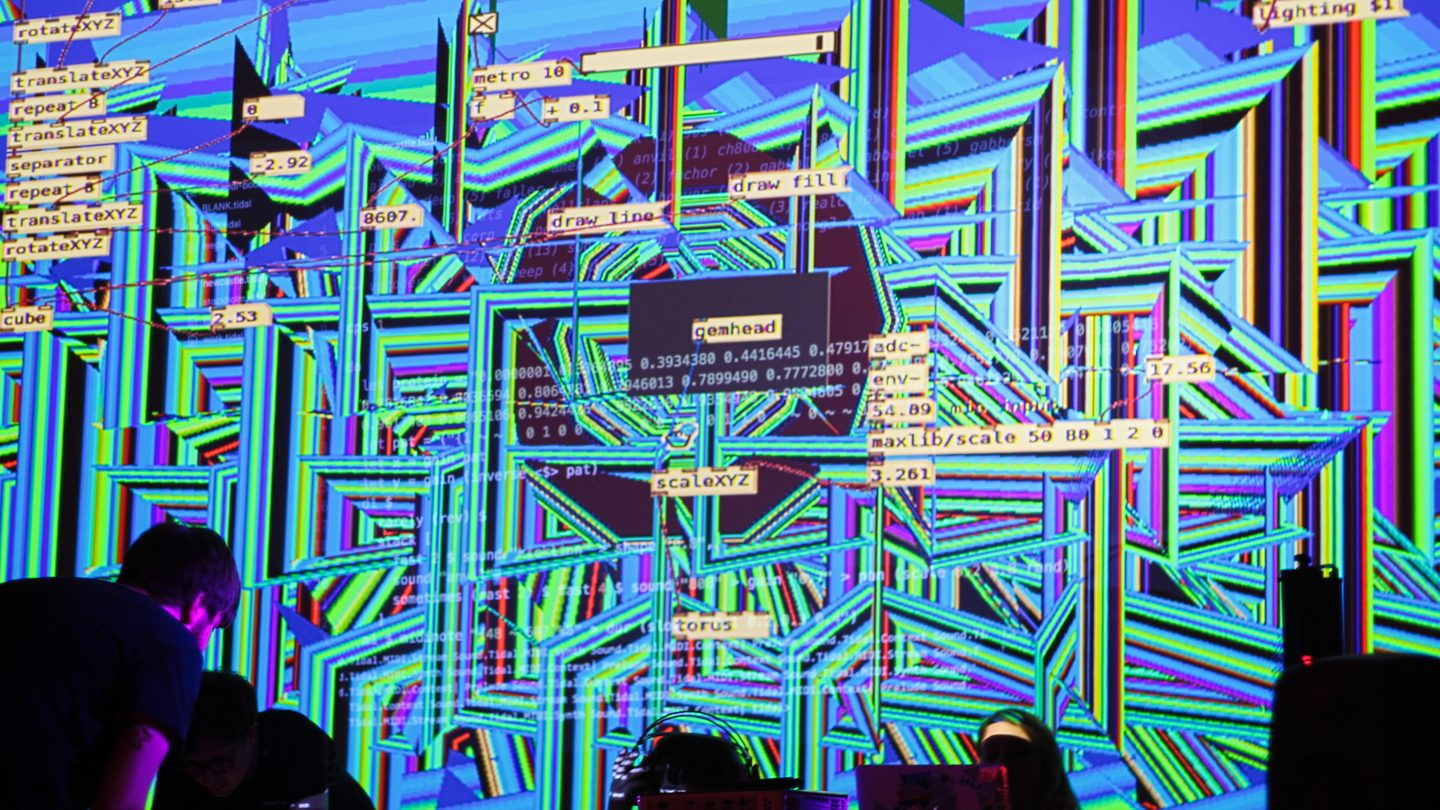
\includegraphics[width=.5\textwidth]{img/Algorave3_ByAntonioRoberts-1440x810.jpg}
	}
\end{center}

%\vspace{0cm}
%{
%\tiny
%\hfill \textcopyright Photos: Antonio Roberts\\
%\hfill \url{noahstroehle.com/amplifying-presence}\\
%\hfill \url{-algorave-at-sxsw-2019/}
%}

\hfill \conclude~Conference on \textbf{Live Coding} (ICLC)
\end{frame}

\begin{frame}[t]{VI. \dimSixTitle}{MuseBots (2015)}
	\centering
	\begin{columns}
		\begin{column}{0.1\textwidth}
		\end{column}
		\begin{column}{0.45\textwidth}
			\underline{Idea}: a unified protocol for interconnecting various musical \emph{agents}
			\bigskip
			
			\begin{quote}
				\enquote{A musebot is here defined as a \textbf{piece of software that autonomously creates music collaboratively with other musebots}. Our project is concerned with putting together musebot ensembles} {\normalfont\citep{MuseBots}}
			\end{quote}
		\end{column}
		\begin{column}{0.1\textwidth}
		\end{column}
		\begin{column}{0.6\textwidth}
			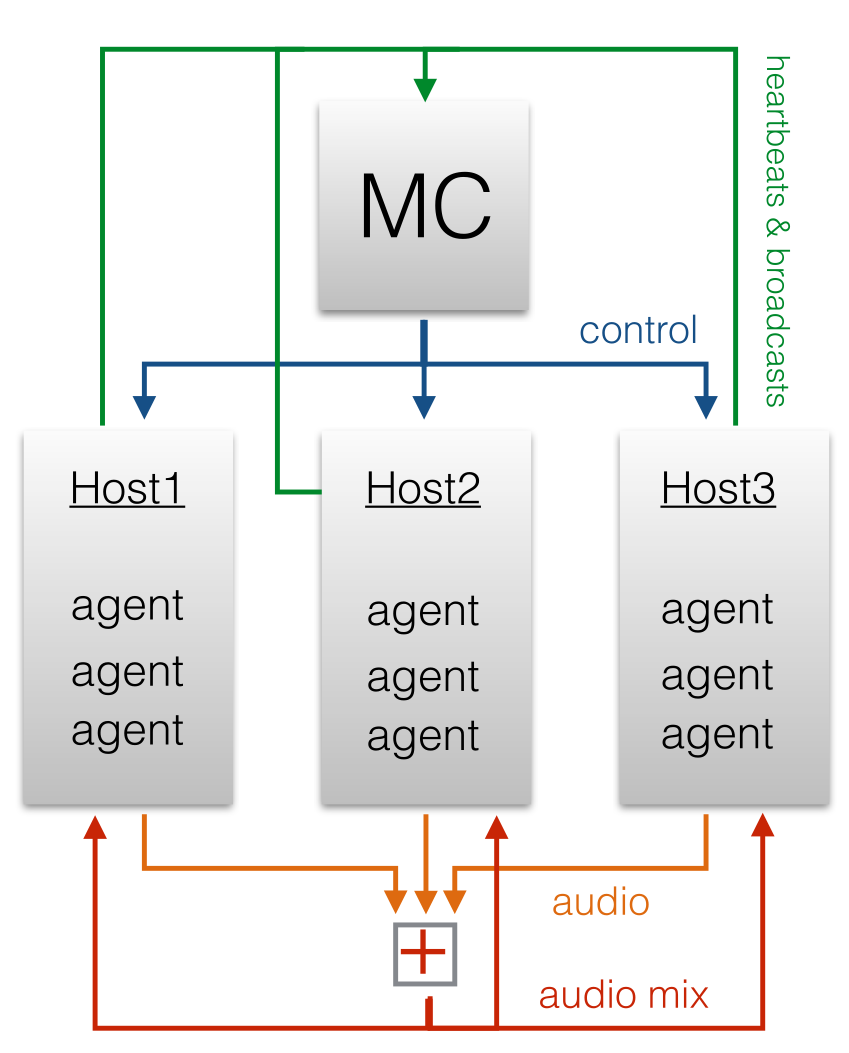
\includegraphics[height=.7\textheight]{img/MuseBots_MC.png}
		\end{column}
	\end{columns}
\end{frame}

%%%%%%%%%%%%%%%%%%%%%%%%%%%%%%%%%%%%%%%%%%%%%%%%
%%%%%%%%%%%%%%%%%%%%%%%%%%%%%%%%%%%%%%%%%%%%%%%%
\section{Evaluation of \enquote{Creative} Systems}

\begin{frame}{Objective Evaluation}
%	\todobox{ein paar Maße zeigen, mit Mathe und Beispiel!!}
	
	\begin{center}
		\fbox{\Large Formalism~~~vs.~~~Dataset Comparison}
	\end{center}
	\bigskip

	\warnSign~Usefulness? Unclear.\\
	\smallskip
	~~~~\conclude~If a metric on aesthetics could be found that is \enquote{objectively correct},\\
	\hfill \emph{automatic composition} would be solvable as an \textbf{optimization problem}\\\hfill(e.g., with an EA)!\\
	\bigskip
	
	Rather: heuristics can be used as necessary conditions, but not as sufficient explanation.
	\bigskip
	
	\hfill \conclude International Conference on \textbf{Computational Creativity} (ICCC)
\end{frame}

\begin{frame}{Subjective Evaluation}
	\drawat{10.5cm,3cm}{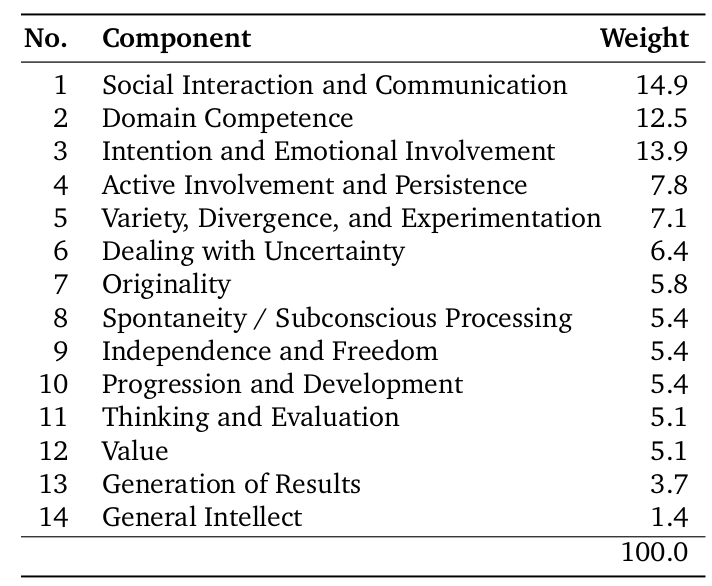
\includegraphics[height=.45\textheight]{img/SPECS_Components.png}}
	
	\underline{Approaches}
	\begin{itemize}
		\item Qualitative surveys (e.g., Likert scale ratings, or pair-wise rankings)
		\item Variants of \textbf{musical Turing tests} (\emph{Imitation Game})
		\item Standardized system evaluation, e.g., SPECS: \citep{SPECS}\\
		\medskip
		\parbox{8cm}{
			\begin{enumerate}
				\item \emph{Computational
				linguistics analysis} clusters 14 components from academic papers on the topic of \emph{creativity}
				\smallskip
				\item A blind survey on the term \enquote{musical improvisational creativity} yields weights
			\end{enumerate}
		}
	\end{itemize}
	
	\bigskip\medskip
	\warnSign~A problem for survey studies with humans:\\
	\smallskip
	~~~\emph{Categorical rejection} (negative bias) against AI music \citep{AIComposerBias,AIPerformerBias}\\
	\smallskip
	\hfill\conclude~can already be problematic when announcing/advertising a study
\end{frame}

%%%%%%%%%%%%%%%%%%
%%%%%%%%%%%%%%%%%%
\section{Focus: Deep Learning}

\begin{frame}{Current (Research \& Industry) Focus}%{\enquote{What does intelligence even mean here?}}
	\drawat{11.5cm,2.8cm}{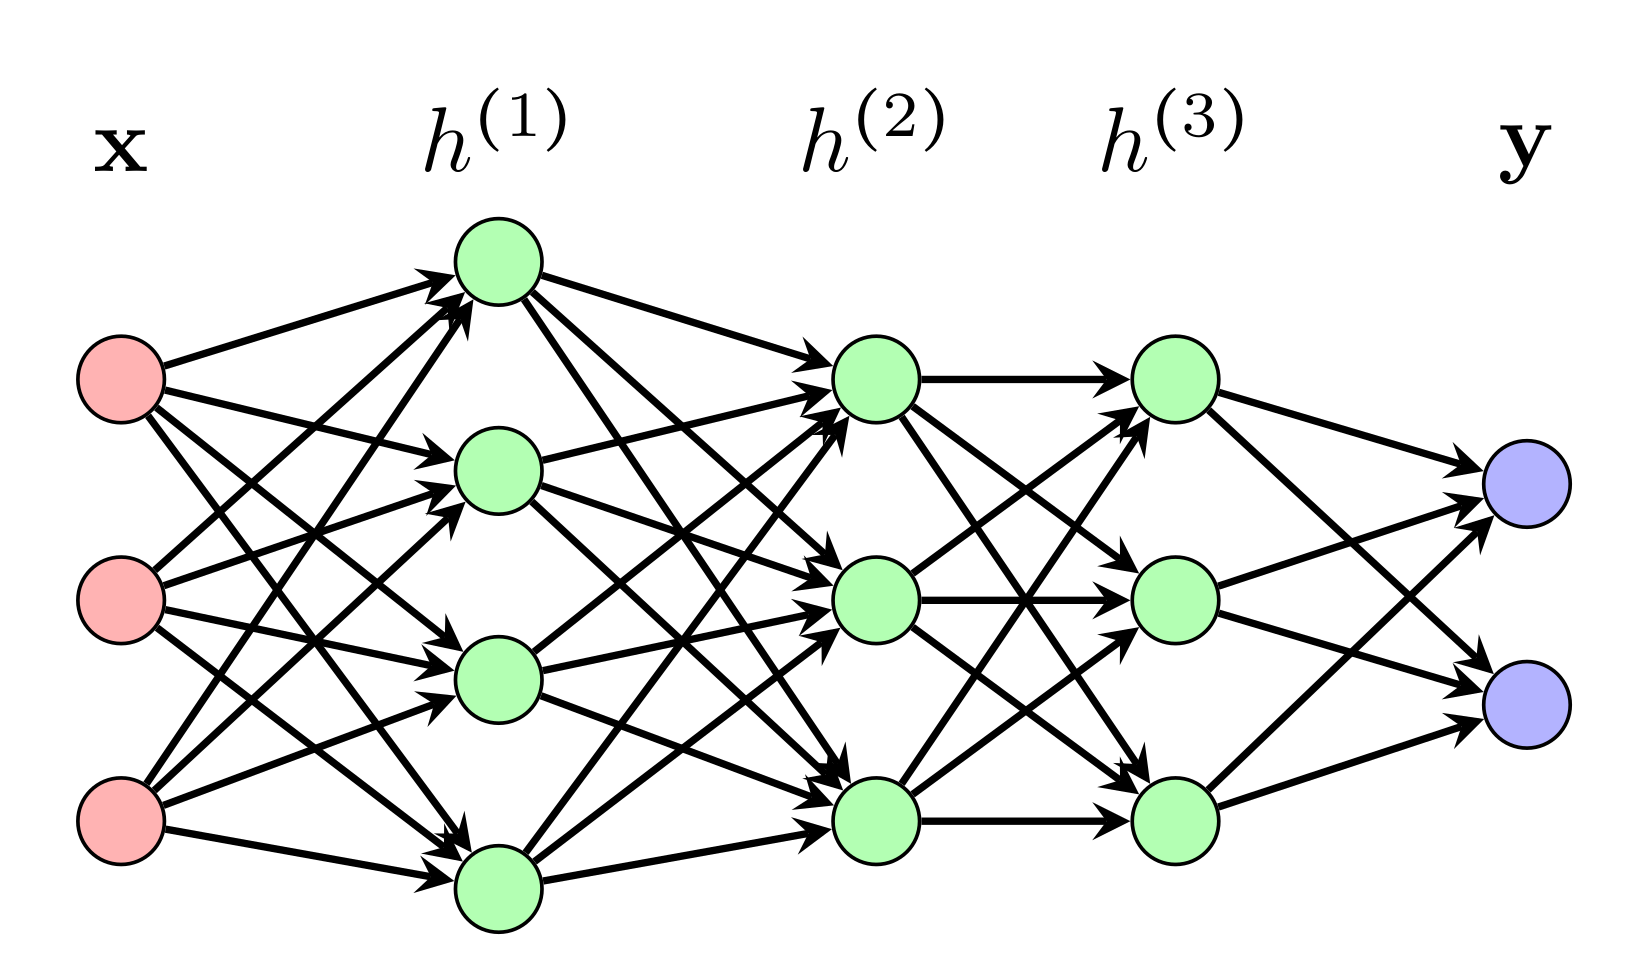
\includegraphics[width=4cm]{img/MLP-Theorie.png}}
	So-called \enquote{Artificial Intelligence} \warnSign
	\bigskip
	
	What is actually meant: \textbf{Deep Learning} = deep (huge$^*$) \emph{neural networks}
	\bigskip
	
	Popular methods:
	\begin{itemize}
		\item Variational Autoencoder (VAE)\\
			\qquad\conclude~encoder-decoder structure
		\item Generative Adversarial Network (GAN)\\
			\qquad\conclude~zero-sum game between generator and discriminator
		\item Diffusion Models\\
			\qquad\conclude~denoising of a random initial input
		\item Transformer models\\
		\qquad\conclude~a topic for an entire seminar of its own...
	\end{itemize}

	\hfill \footnotesize $^*$easily $10^6$--$10^{12}$ parameters
\end{frame}

\begin{frame}{Variational Autoencoder}{(VAE)}
	\begin{columns}
		\begin{column}{.5\textwidth}
			\underline{Autoencoder}:\\
			\raggedleft
			Each known data point = one point in the \emph{latent} space\\
			\vspace{-.2cm}
			\includegraphics[width=.9\textwidth]{img/MLP/MLP_autoencode.pdf}
		\end{column}
		\begin{column}{.5\textwidth}
			\underline{Variational Autoencoder}:
			\medskip
			
			\raggedleft
			Each known data point = a distribution in the latent space\\
			\raggedright
			\[z \sim \mathcal{N}(\mu(x), \sigma^2(x))\]
			
			Backpropagation is made possible by the \enquote{reparametrization \underline{trick}}:\\
			\[z = \mu(x) + \sigma(x) \cdot \epsilon\]
			
			$\mu$ and $\sigma$ are learned\\
			$\epsilon$ is varied during training\\
			\medskip
			
			\Conclude~Variation of musical elements is a well-established composing strategy
		\end{column}
	\end{columns}
\end{frame}

\begin{frame}{Generative Adversarial Network}{(GAN)}
	\centering
	\includegraphics[width=0.7\textwidth]{img/gan_schematic.pdf}
	
	\vfill
	\hfill\scriptsize Image source: \url{https://doi.org/10.23889/ijpds.v8i1.2158}
\end{frame}

\begin{frame}[t]{Diffusion Models}
	\vspace{-1cm}
	\begin{center}
		\includegraphics[width=\textwidth]{img/Diffusion/DiffusionModel.pdf}
	\end{center}
	\small
	
	Idea: step-by-step \emph{denoising} of a random input
	\medskip
	
	$q$: adding noise to the dataset (inversion intractable)\\
	$p_\theta$: estimated (learned) \emph{denoising} function
	\medskip
	
	Particularly interesting: \textbf{partial reconstruction} \conclude~\enquote{inpainting}
	
	\drawat{11.5cm,5.5cm}{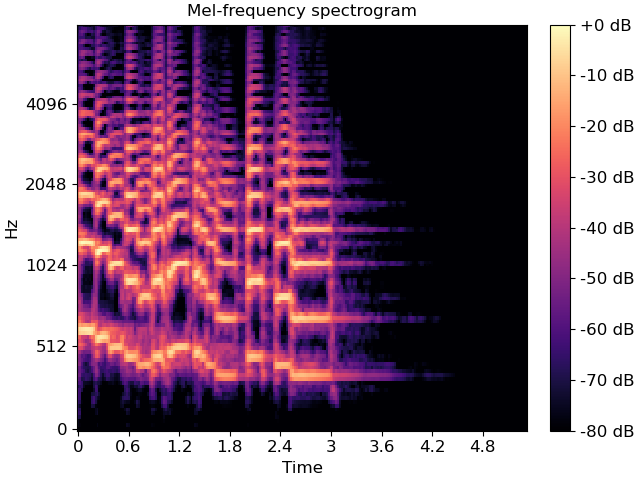
\includegraphics[height=2.8cm]{img/librosa-feature-melspectrogram-1.png}}
\end{frame}

\begin{frame}{Transformer}{MIDI-GPT (2025)}
	\begin{center}
		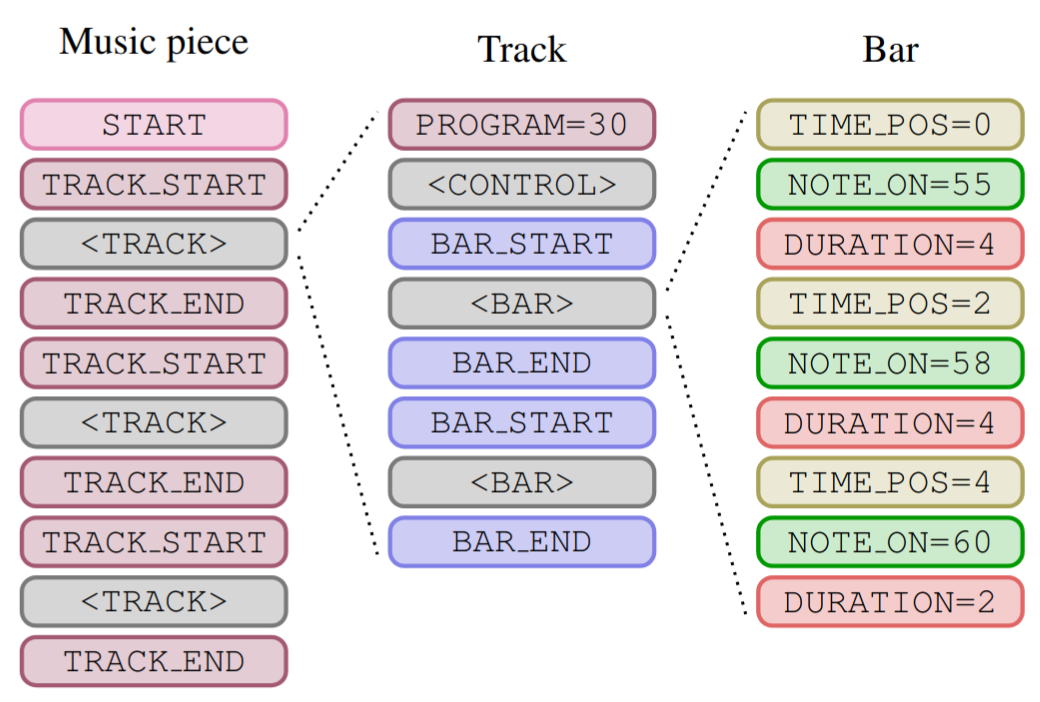
\includegraphics[width=.6\textwidth]{img/MidiGPT.png}
	\end{center}
\end{frame}

\begin{frame}{Transformer}{MusicLM (2023)}
	\begin{center}
		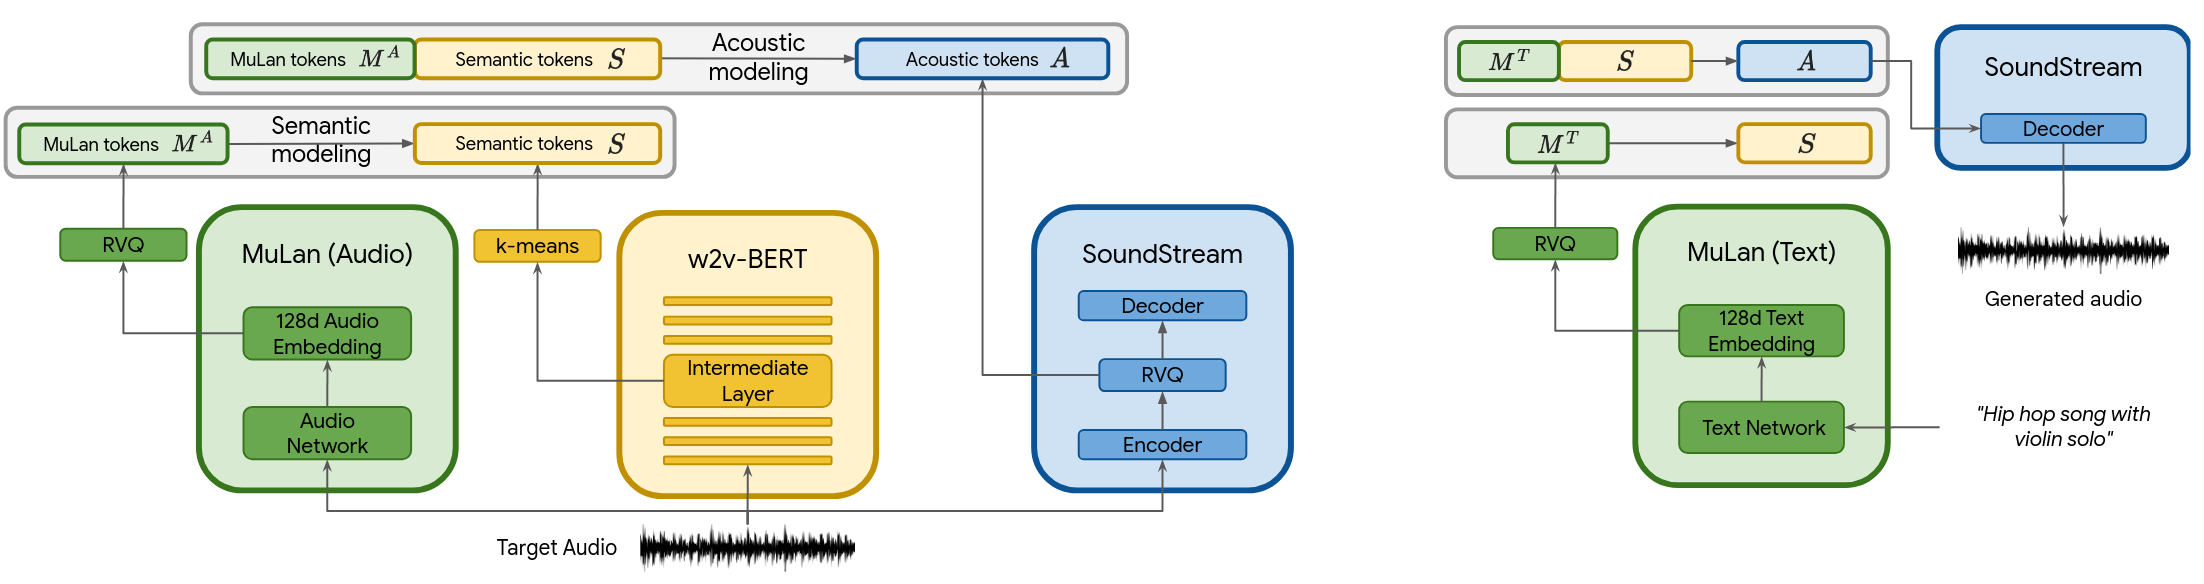
\includegraphics[width=1\textwidth]{img/MusicLM.png}
	\end{center}
	
	\hfill\Conclude~Still, we have not reached \enquote{photo-realism} for music generation\\
	\hfill(our ears are incredibly sensitive)
\end{frame}

\HIDE{
\begin{frame}
\todo[inline]{LLM-based composers?}
\end{frame}
}

\begin{frame}{Deep Learning Systems}
		Classification:
		\begin{itemize}
			\item data-driven
			\item stochastic\\
			~~~\conclude~{\small(deterministic for a fixed input)}
			\item (digital) representation depends heavily on the dataset\\
			~~~\conclude~{\small score or sound possible}
			\item (mostly) not interactive
			\item not (yet) real-time capable
			\item Objective: mostly \emph{end-to-end}
		\end{itemize}
		
		\vspace{-2.75cm}
		\hfill Further reading: \raisebox{-\baselineskip}{\hspace{-.6cm}\citep{DL4music}~~}
		\raisebox{-1.6cm}{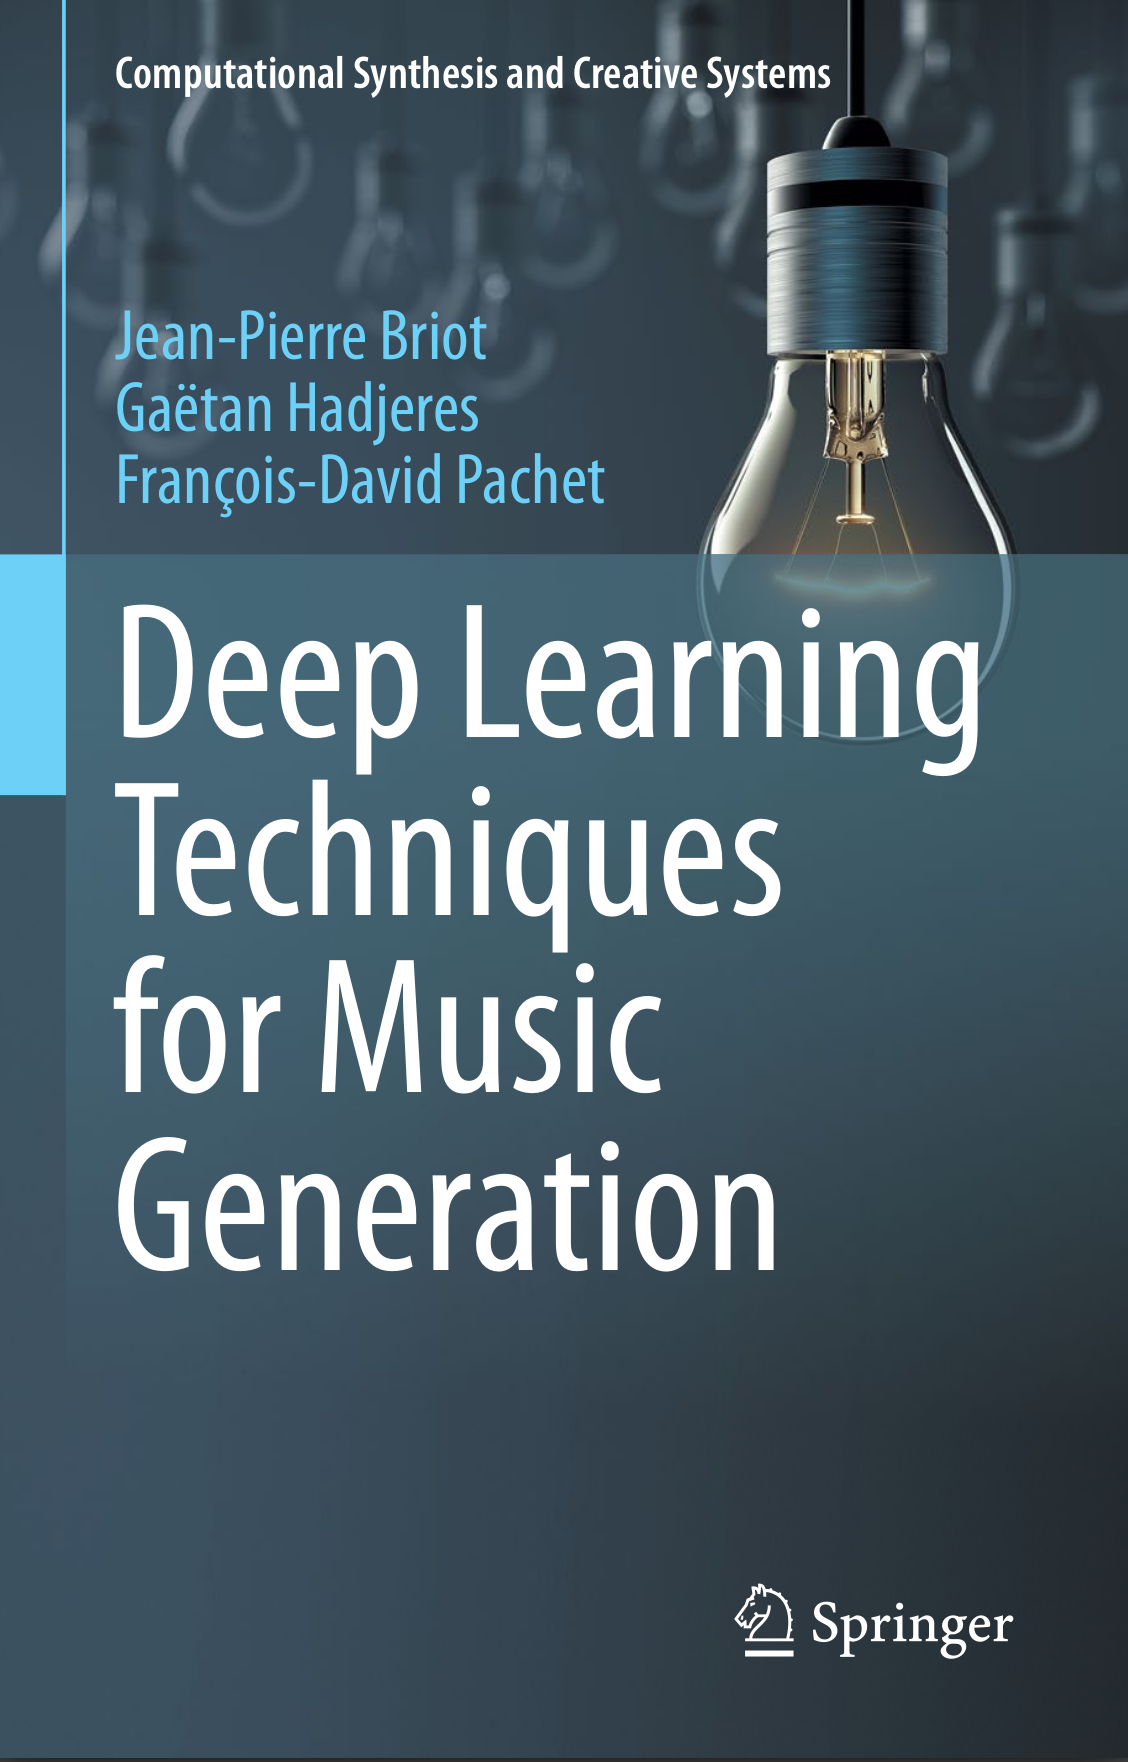
\includegraphics[height=4.5cm]{img/DL4music_cover.png}}
		
		\vspace*{-.5cm}
		\centering \conclude~Conference on \textbf{AI Music Creativity} (AIMC)~~~
\end{frame}

\begin{frame}{Hierarchical Categorization by Method}{(as of 2014)}
	\centering
	\includegraphics<1>[height=.75\textheight]{img/AI_Methods_For_AlgoComp_Overview.png}\includegraphics<2>[height=.75\textheight]{img/AI_Methods_For_AlgoComp_Overview_mark.png}\citep{FernandezVico2013}
\end{frame}

\begin{frame}{The Future?}{Prompt-Based Systems}
	
	\underline{DALL-E 2}: \enquote{An Astronaut Riding A Horse}\\
	\smallskip
	\resizebox{1.075\textwidth}{!}{
		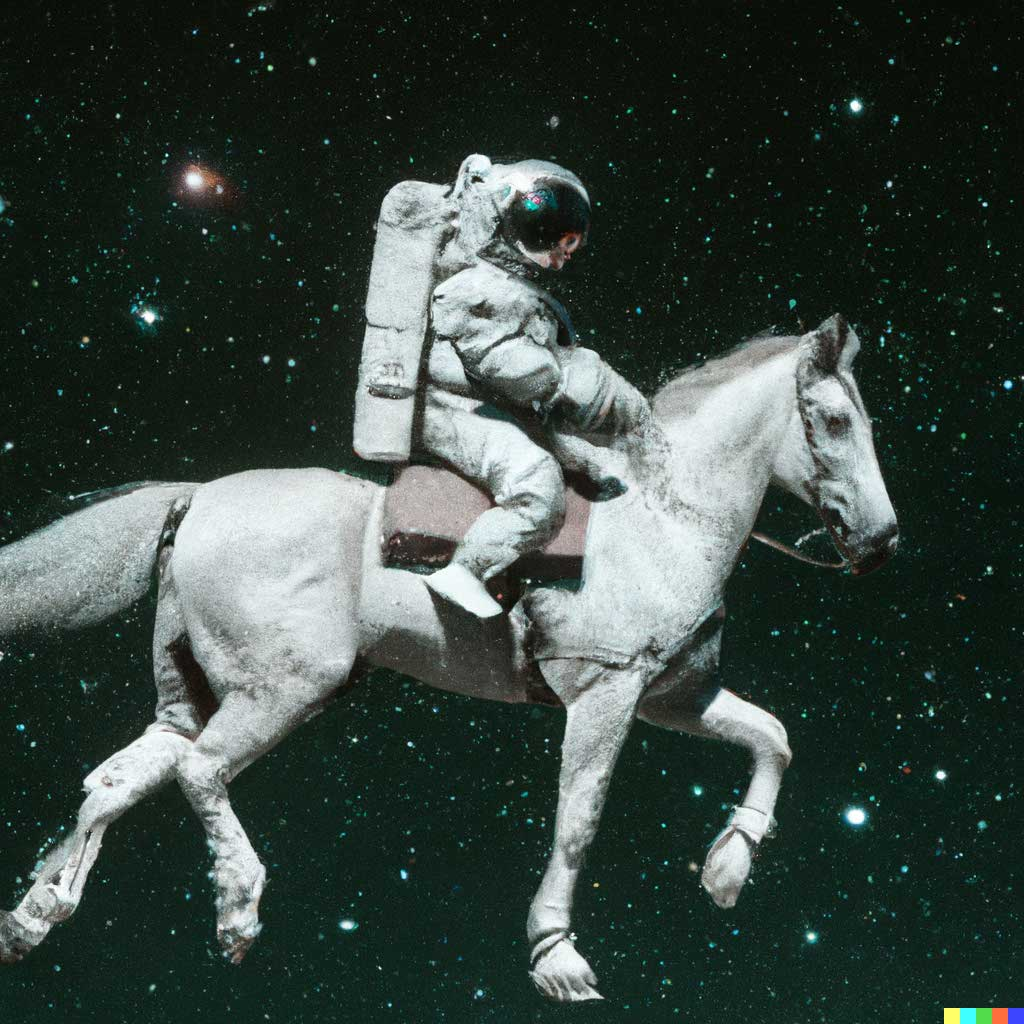
\includegraphics{img/Dalle2-AstronautRidingHorse/0.jpg}
		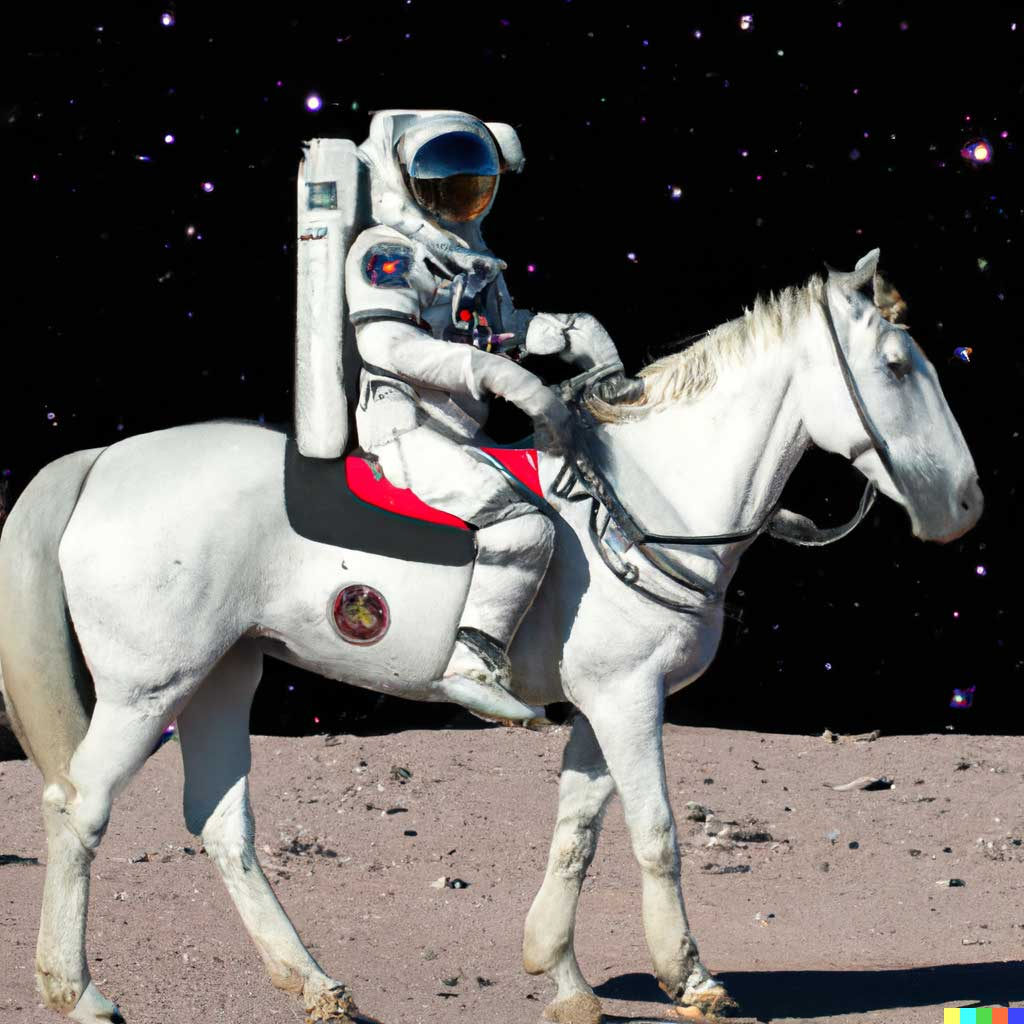
\includegraphics{img/Dalle2-AstronautRidingHorse/1.jpg}
		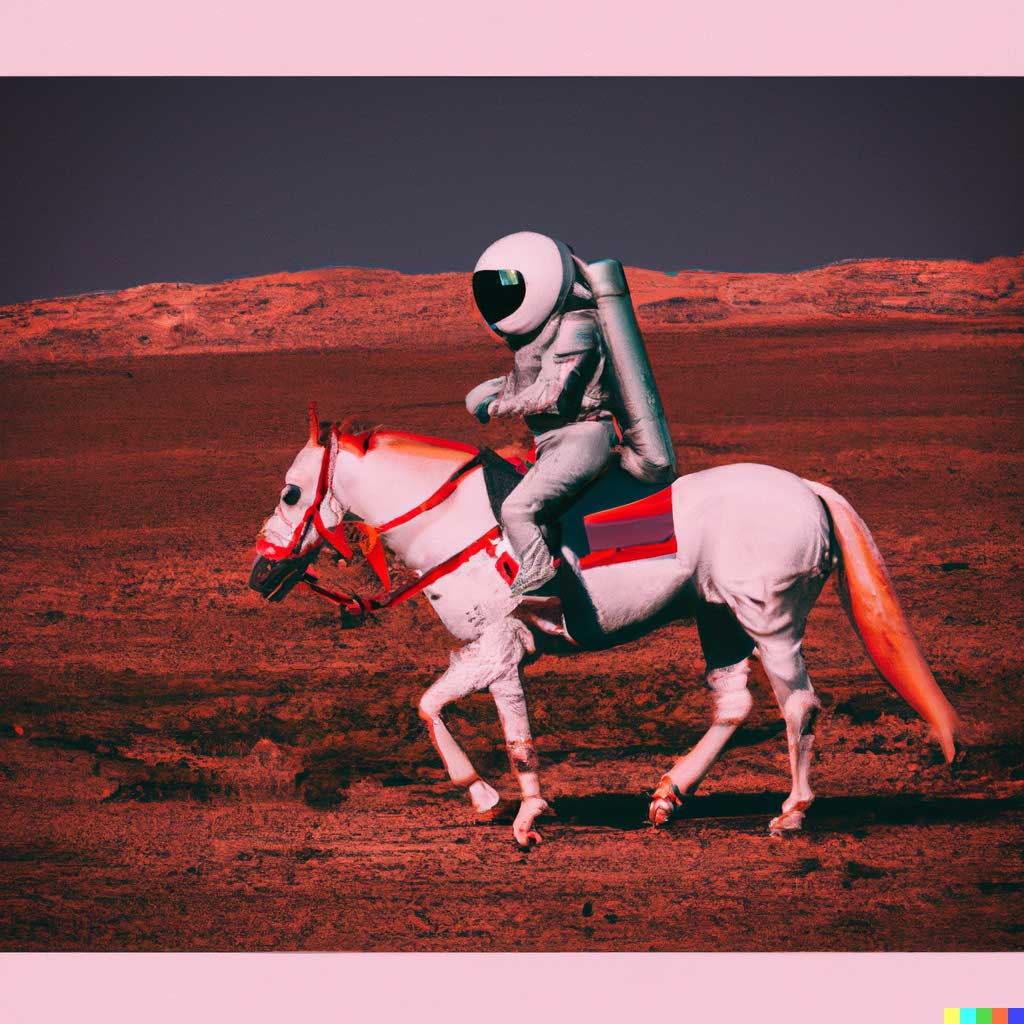
\includegraphics{img/Dalle2-AstronautRidingHorse/2.jpg}
		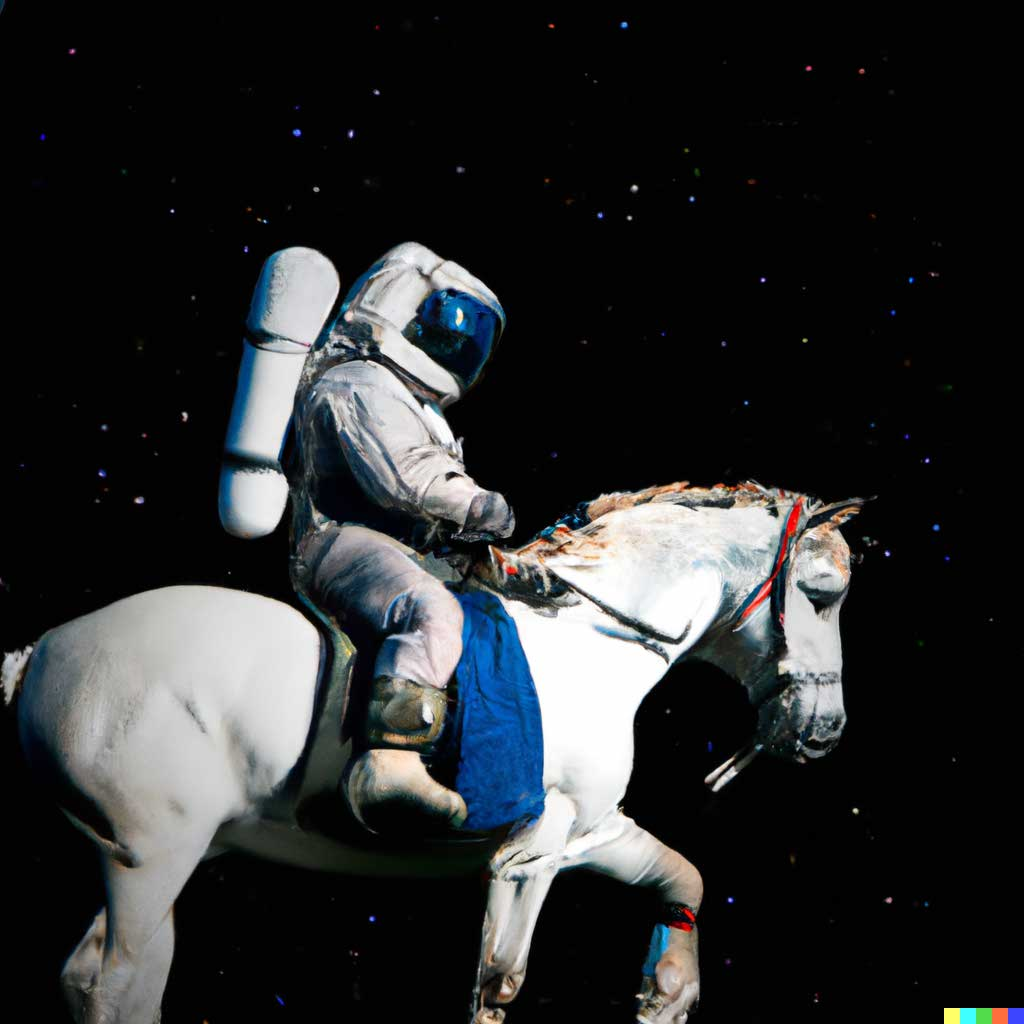
\includegraphics{img/Dalle2-AstronautRidingHorse/3.jpg}
		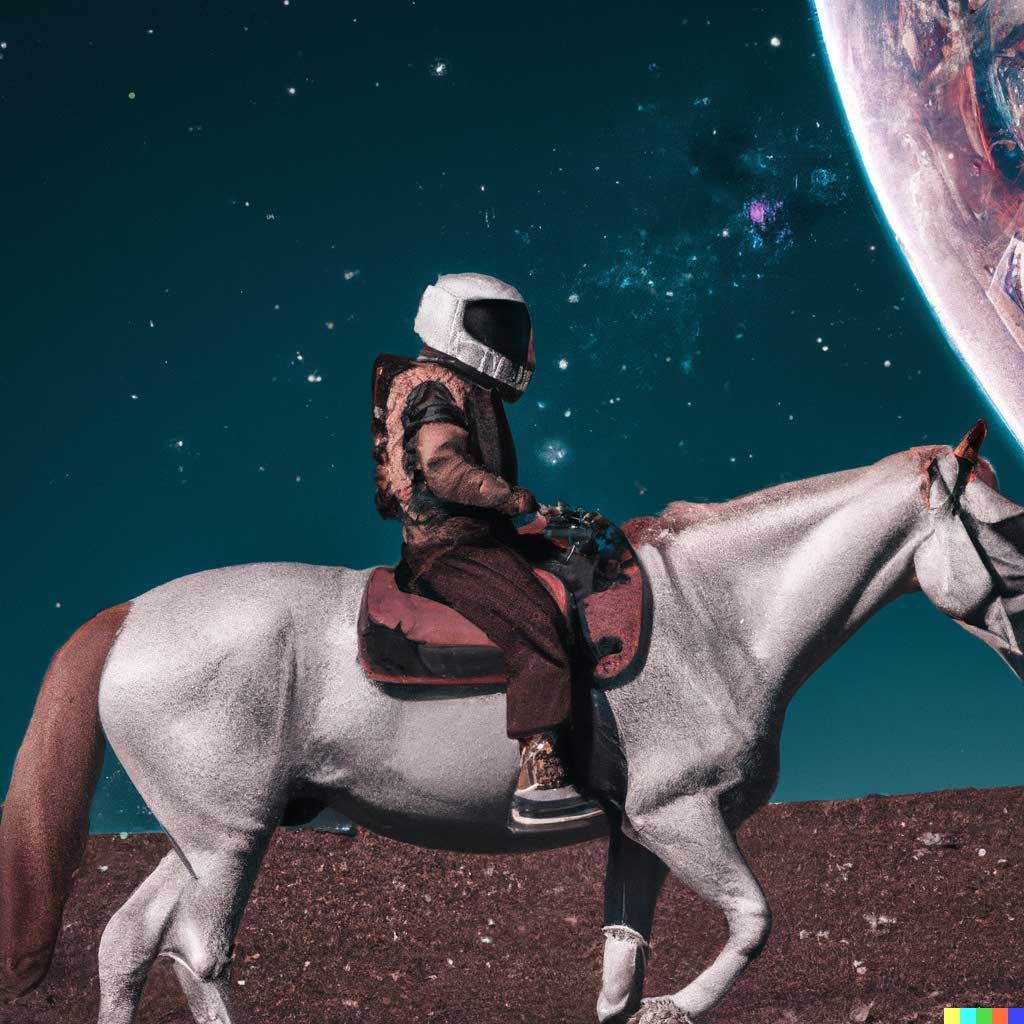
\includegraphics{img/Dalle2-AstronautRidingHorse/5.jpg}
		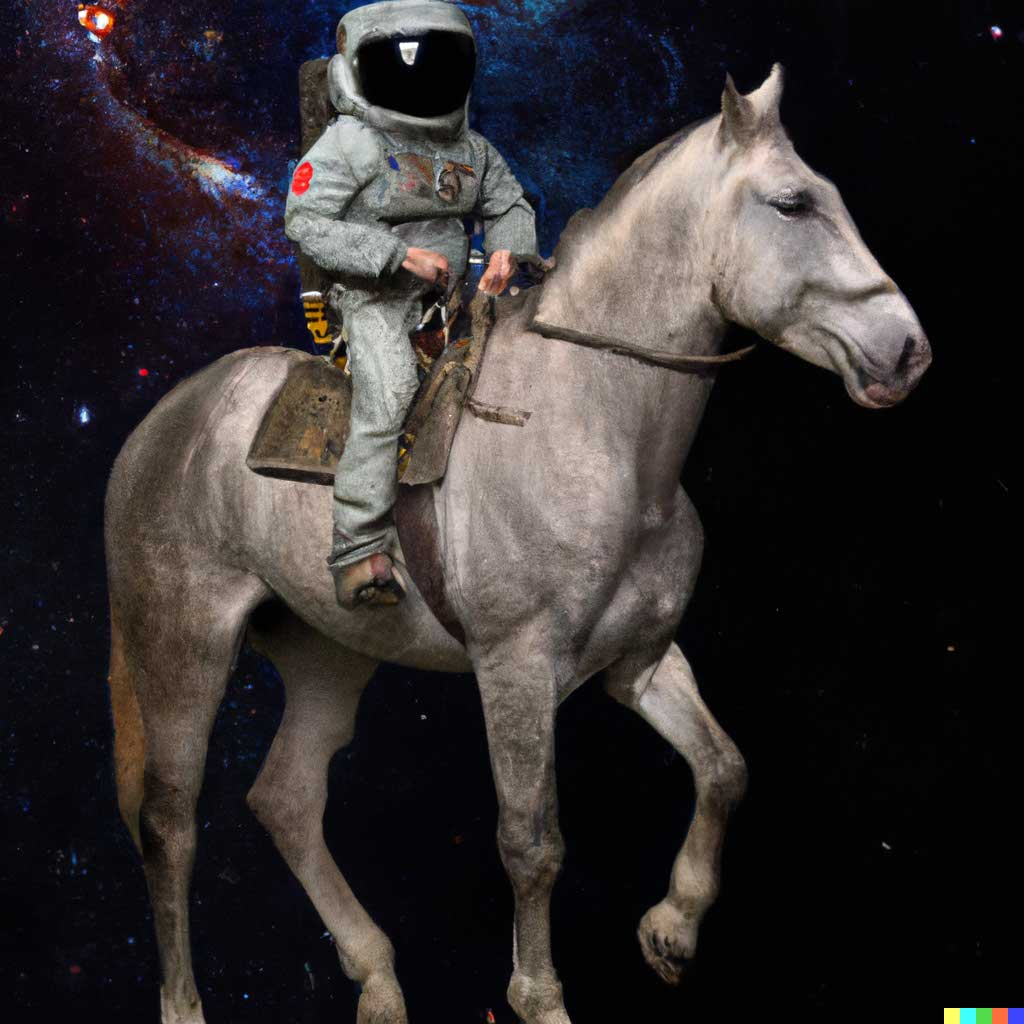
\includegraphics{img/Dalle2-AstronautRidingHorse/7.jpg}
		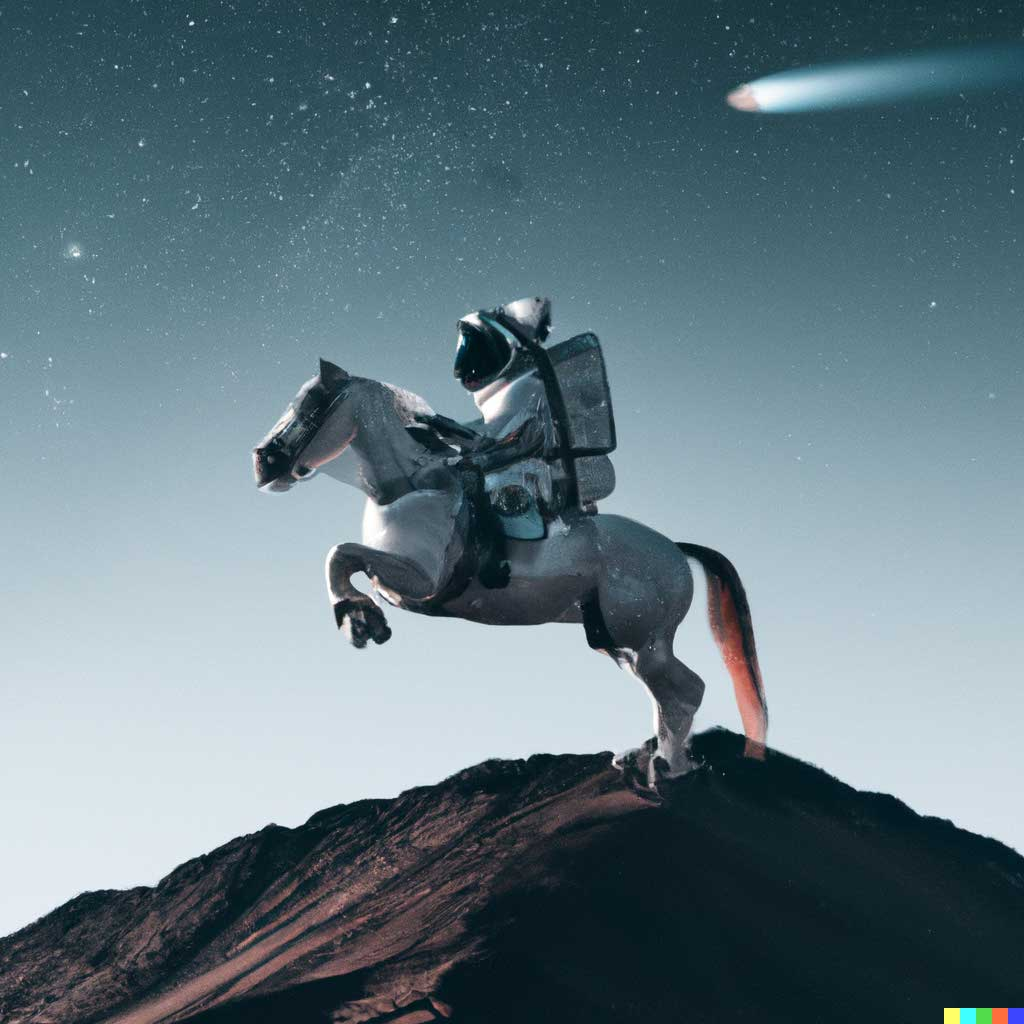
\includegraphics{img/Dalle2-AstronautRidingHorse/9.jpg}
	}
	\medskip
	Prompt-based models for music exist, e.g., MusicLM \& StableAudio.\\ 
	
	\bigskip
	\hfill \underline{The open question remains}: \enquote{What will these systems be unable to learn?}\hspace{-.5cm}	
\end{frame}

\begin{frame}{Copyright?}
	\vspace{-.2cm}
	\tiny
	\begin{columns}
		\begin{column}[t]{.5\textwidth}
			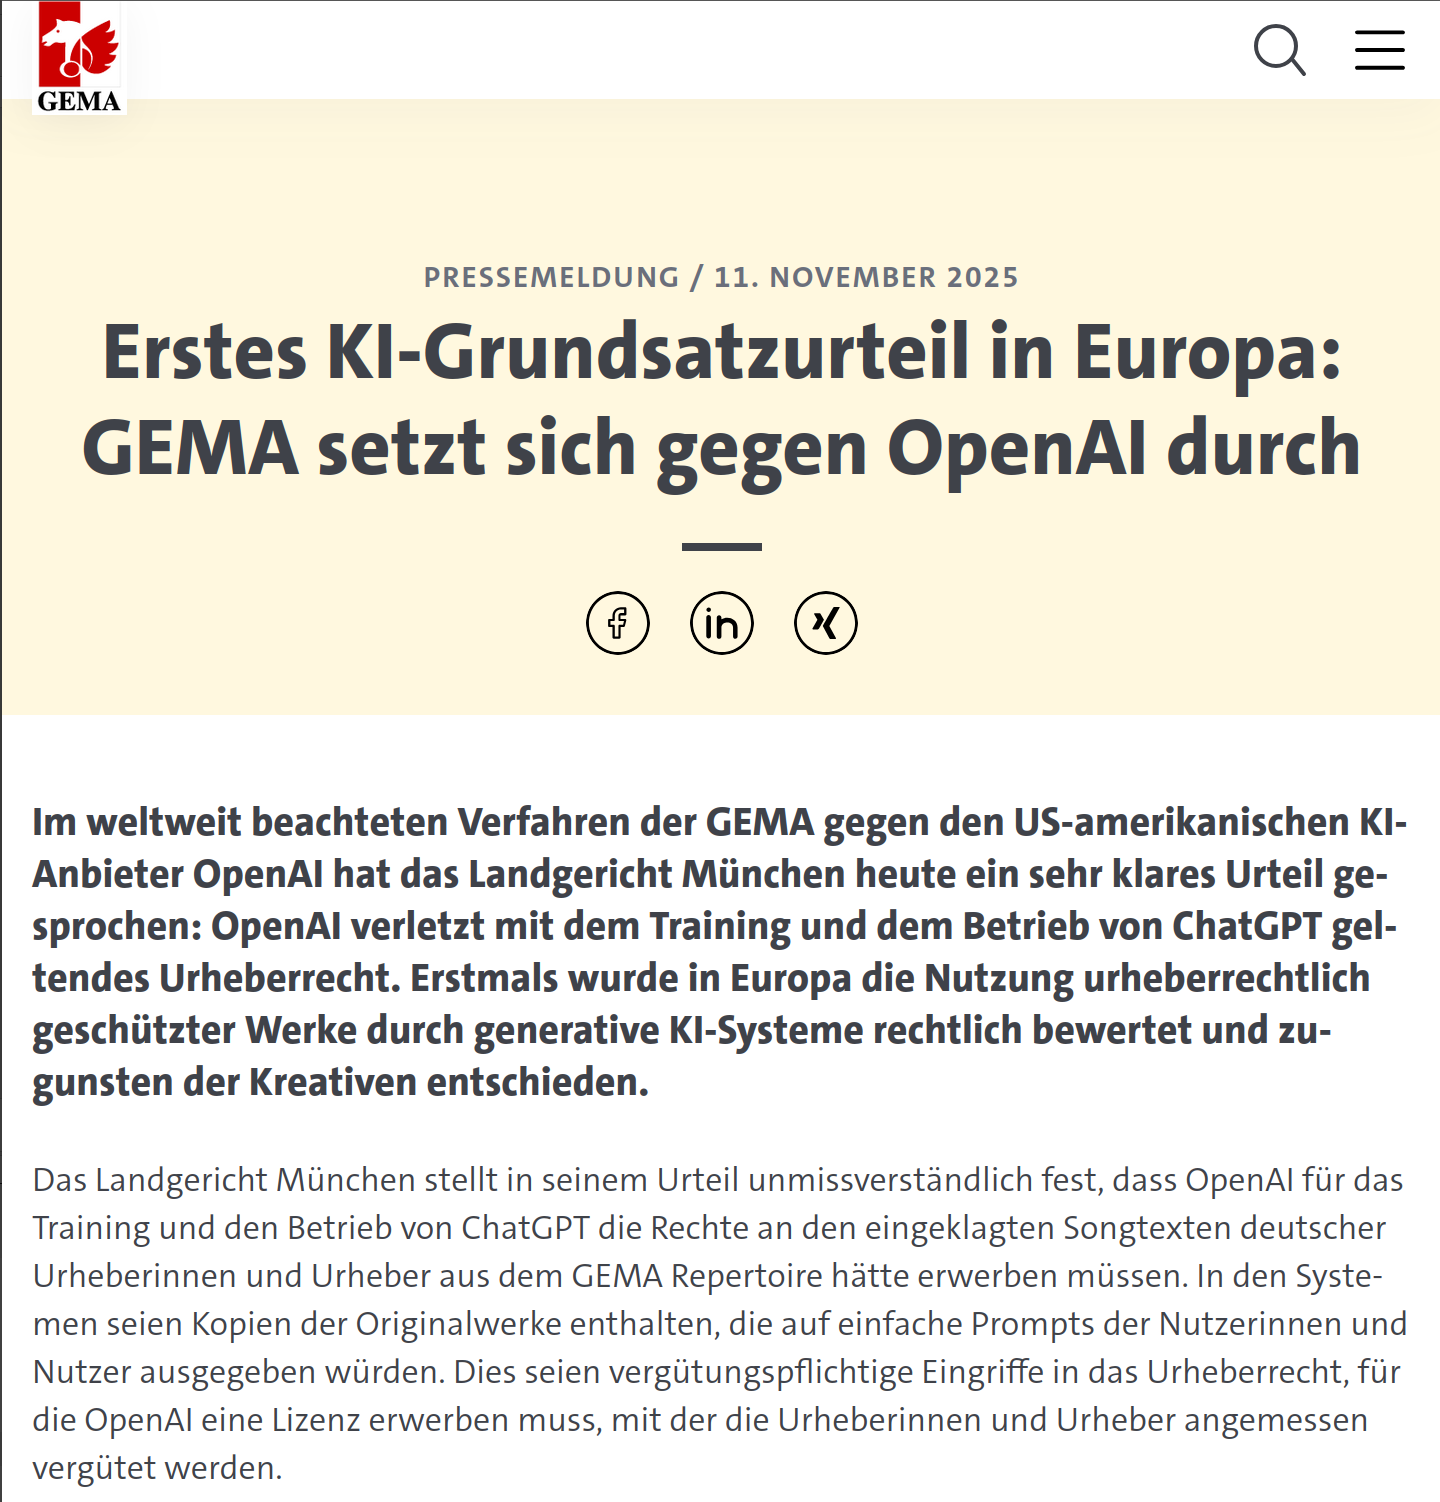
\includegraphics[width=.96\textwidth]{img/Gema-wins-openai.png}
			\url{https://www.gema.de/de/w/grundsatzurteil-gema-gegen-openai}
		\end{column}
		\begin{column}[t]{.5\textwidth}
			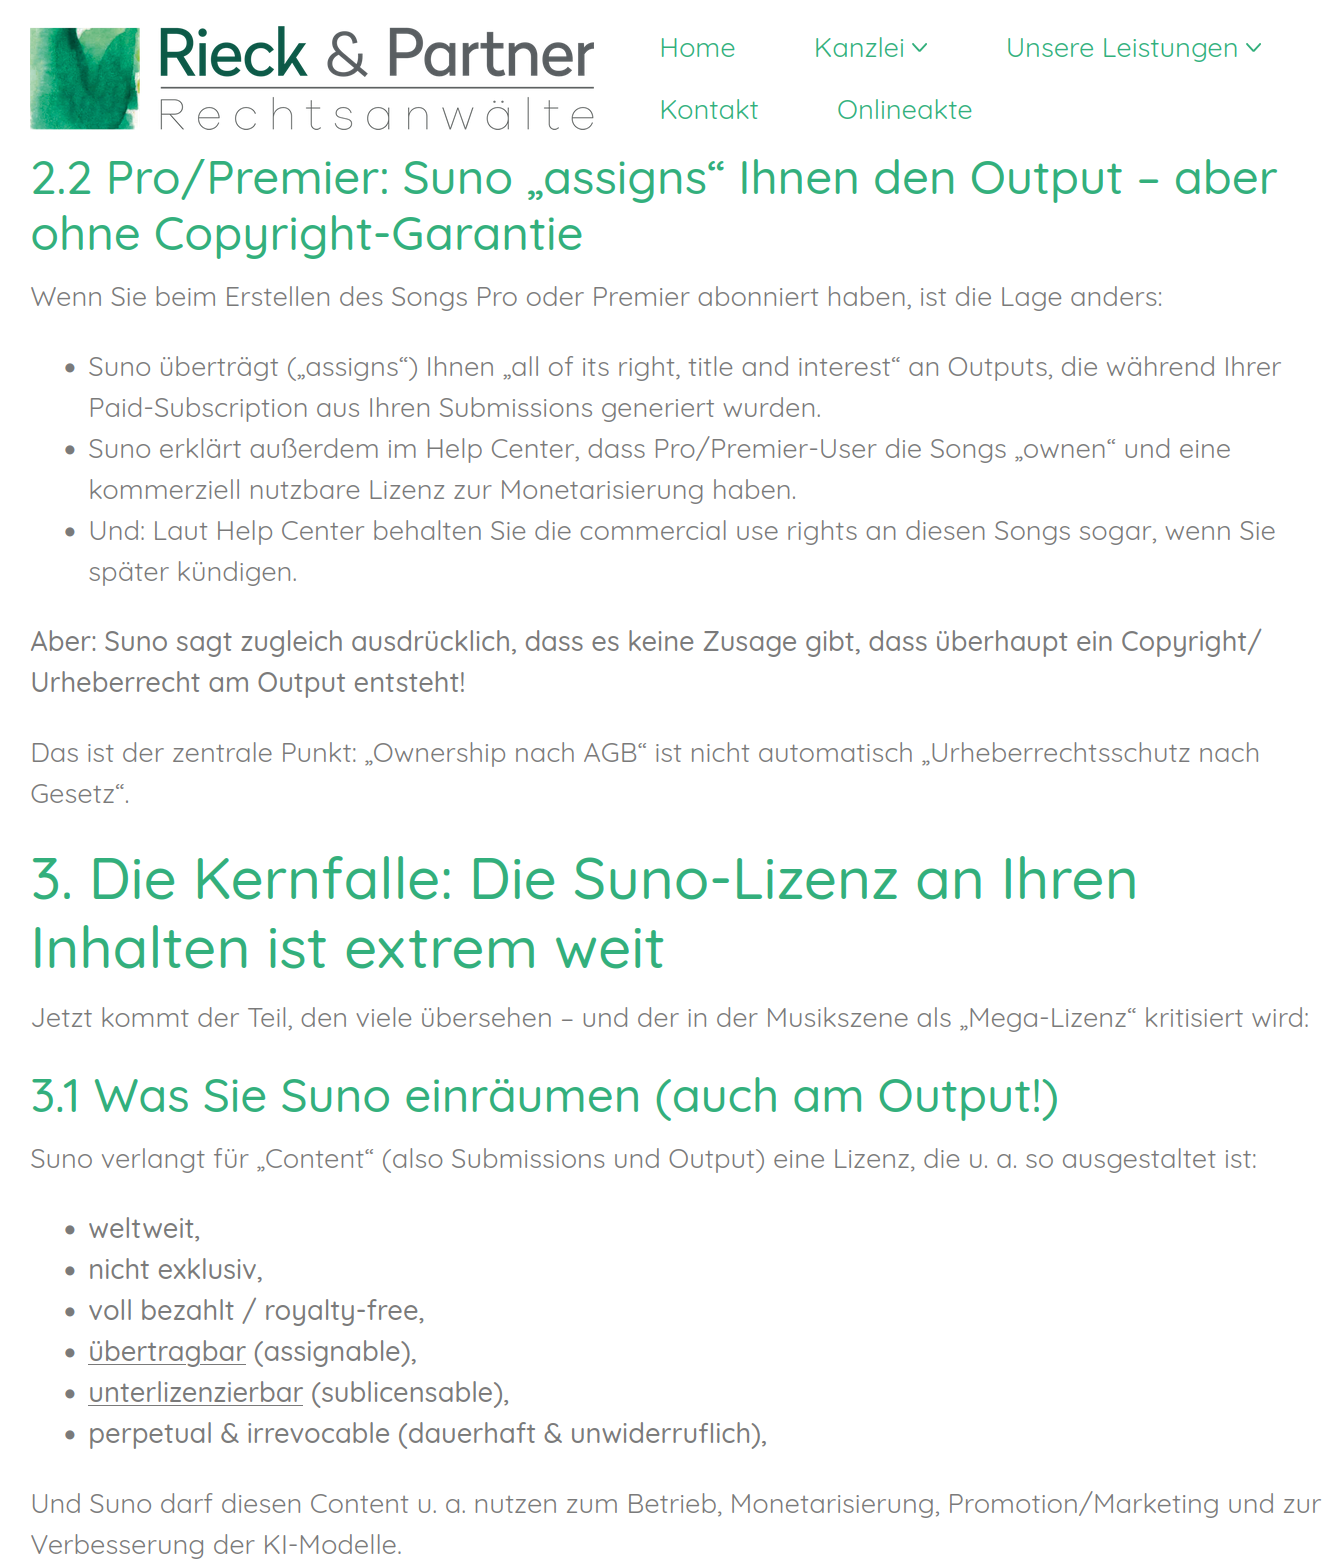
\includegraphics[width=.88\textwidth]{img/Suno_AGB_Analyse.png}
			\url{https://rieck-partner.de/musik/suno-ai-nutzungsbedingungen-urheberrecht-wem-gehoeren-ki-songs.html}
		\end{column}
	\end{columns}
\end{frame}

\begin{frame}[t]{How to overcome the problem of originality?}{Reinforcement Learning with Human Feedback}
	\vspace{-.2cm}
	\begin{center}
		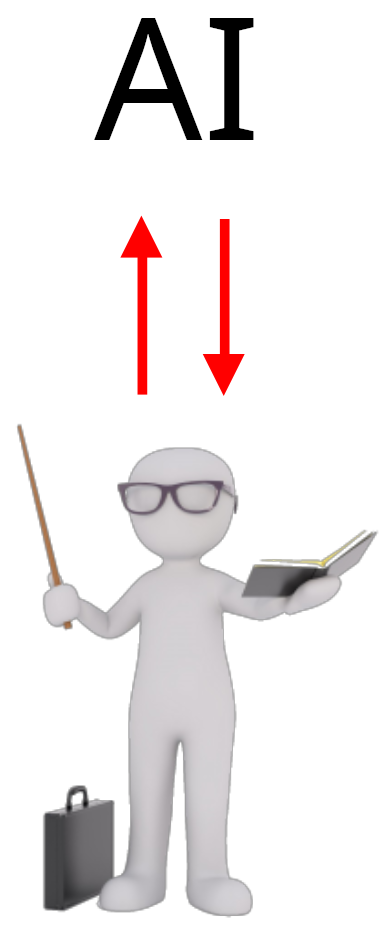
\includegraphics[height=.75\textheight]{img/RLHF-icon_english.png}~~~~
	\end{center}
	\vspace{-3cm}
	\hfill\conclude~counteracts \emph{model collapse} \cite{ModelCollapse}
	
	\bigskip
	\hfill\parbox{.38\textwidth}{(idea similar to \emph{GenJam},\\replacing evolutionary algorithms with reinforcement learning)}
\end{frame}

\HIDE{
\begin{frame}{Held Horizon (2025)}{AI–human co-creation experiment on composing for choir}
	\centering
	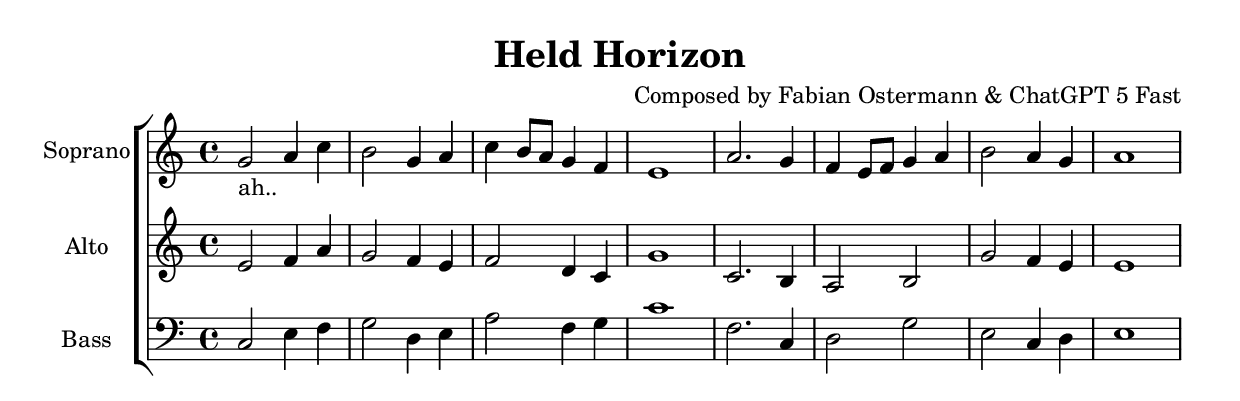
\includegraphics[width=.95\textwidth]{img/HeldHorizon_SAB_crop.png}
	\vfill
	Explanations and transcript of the \enquote{composition dialogue}:\\
	\hfill\scriptsize\url{http://fabianos.org/content/2025/09/11/Held-Horizon}
\end{frame}
}
 %%%%
%%%%%%%%%%%%%%%%%%%%%%%%%%

%% !TeX root = MDA_VL_Ostermann.tex
%%%%%%%%%%%%%%%%%%%%%%%%%%%%%%%%%%%%%%
%%%%%%%%%%%%%%%%%%%%%%%%%%%%%%%%%%%%%%
\section{Organisatorisches}

\begin{frame}{Hinweise zur Klausur}
	\underline{Anmeldung zur 1. Klausur}:\\\smallskip
	
	\textbf{Informatiker} melden sich per \textbf{BOSS} an.
	\medskip
	
	\textbf{Alle anderen} schreiben eine \textbf{Email} (an \url{guenter.rudolph@tu-dortmund.de})\\
	unter Angabe von\\
	
	\begin{itemize}
		\item Name, Vorname, Matrikelnummer, Studiengang, Klausurtermin\\
	\end{itemize}
	
	\bigskip
	Anmeldeschluss: 7 Tage vor dem Klausurtermin.\\
	\bigskip
	
	\underline{Klausurtermine}:\\\smallskip
	\begin{itemize}
		\item Donnerstag, \textbf{19.02.2026, 10:30--12:00\,Uhr}, Otto-Hahn-Str.\,14, R202.
		\item Donnerstag, \textbf{26.03.2026, 10:30--12:00\,Uhr}, Otto-Hahn-Str.\,14, R202.
	\end{itemize}
\end{frame}

\begin{frame}{Hinweise zur Übung am 5.2.2026}
Geplant als praktisches \textbf{Hands-On} zur Thematik.\\
\bigskip

Empfehlung: \textbf{Ausprobieren} von \textbf{Python} mit \textbf{Scamp}-Library\\

{\small\itshape Aber: Aufgaben sind so gestaltet, dass sie generell auch in R und Matlab lösbar sind.}\\
\bigskip

Übungsaufgaben finden sich ab \emph{jetzt} im \emph{Moodle}.
\bigskip

%Detail-Fragen zu den Inhalten/Folien von heute sind willkommen!
\end{frame}

\begin{frame}{References}%[allowframebreaks] % enable this if references do not fit into one frame
	\bibliographystyle{unsrtdin} %unsrtdin or natdin
	%\nocite{*}
	{%\tiny
		\fontsize{5}{6}\selectfont %<- makes it ultra tiny!
		\bibliography{Literatur.bib}}
\end{frame}


\immediate\closeout\slideinfofile
\end{document}
